\appendix

\chapter{Technical Proofs}
\label{appendix:technical-proofs}

This appendix collects the technical arguments that support the convergence and estimator results used in Chapter~\ref{chapter:methodology}. They are kept here to preserve the flow of the main text while keeping the derivations available.

\section{Canonical Construction}
\label{appendix:canonical-construction}

We work on a probability space rich enough to support the following independent random variables:
\begin{enumerate}
    \item an initial variable $\xi\sim\mu_0$;
    \item transition noises $(\epsilon_t)_{t=1}^{T}$ with common law $\rho\in\Pc(E)$;
    \item policy noises $(\tilde\epsilon_t)_{t=0}^{T-1}$ with common law $\tilde\rho\in\Pc(\tilde E)$;
    \item perturbation variables $(f_t)_{t=0}^{T}$ with common law $\nu\in\Pc(\mathsf F)$.
\end{enumerate}
By the representation theorem for probability kernels of Kallenberg \cite{kallenberg1997foundations}, the transition kernel can be represented by measurable maps $\Xc\times\Pc(\Xc)\times A\times E \ni(x,m,a,e)\mapsto F_t(x,m,a,e)$ such that $F_t(x,m,a,\cdot)\sharp\rho=P_t(\cdot\mid x,m,a)$. Similarly, each randomized policy can be represented by measurable maps $\Xc\times\Pc(\Xc)\times\tilde E\ni(x,m,\tilde e)\mapsto\tilde F_t^\theta(x,m,\tilde e)$ such that $\tilde F_t^\theta(x,m,\cdot)\sharp \tilde\rho= \pi_t^\theta(\cdot\mid x,m)$.

\begin{remark}[Canonical construction of the problem]
    The preceding variables can be realized on the canonical product space $\Omega=\Xc\times E^T\times\tilde E^T\times\mathsf F^{T+1}$, endowed with its Borel $\sigma$-algebra and with the product measure
    \begin{align}
        \P(\d\omega)
        =
        \mu_0(\d x_0)
        \rho^{\otimes T}(\d\epsilon_{1:T})
        \tilde\rho^{\otimes T}(\d\tilde\epsilon_{0:T-1})
        \nu^{\otimes(T+1)}(\d f_{0:T}).
    \end{align}
\end{remark}

For a fixed policy $\pi^\theta$, the unperturbed canonical process is defined by
\begin{align}
    \begin{cases}
        X_0^\theta(\omega)=x_0,\\
        \alpha_t^\theta(\omega)
        =
        \tilde F_t^\theta
        \left(X_t^\theta(\omega),\P_{X_t^\theta},\tilde\epsilon_t(\omega)\right),\\
        X_{t+1}^\theta(\omega)
        =
        F_t
        \left(X_t^\theta(\omega),\P_{X_t^\theta},\alpha_t^\theta(\omega),\epsilon_{t+1}(\omega)\right),
    \end{cases}
    \qquad t=0,\ldots,T-1.
\end{align}
By construction, it follows that
\begin{align}
    \begin{cases}
        X_0^\theta\sim\mu_0,\\
        \Lc\left(\alpha_t^\theta\mid X_t^\theta,\P_{X_t^\theta}\right)
        =
        \pi_t^\theta(\cdot\mid X_t^\theta,\P_{X_t^\theta}),\\
        \Lc\left(X_{t+1}^\theta\mid X_t^\theta,\P_{X_t^\theta},\alpha_t^\theta\right)
        =
        P_t(\cdot\mid X_t^\theta,\P_{X_t^\theta},\alpha_t^\theta).
    \end{cases}
\end{align}

\section{Discrete-State Space Proofs}
\label{appendix-discrete_proofs}

\subsection{Perturbation Estimate}
\label{appendix:discrete-perturbation-estimate}

We prove Theorem~\ref{theorem:discrete-perturbation-estimate}.
For every $\omega$, $M_t^{\lambda,\theta}(\omega)-\mu_t^\theta = \lambda(q_t(\omega)-\mu_t^\theta)$, hence $\| M_t^{\lambda,\theta}(\omega)-\mu_t^\theta\|_1 = \lambda\|q_t(\omega)-\mu_t^\theta\|_1\leq 2\lambda$ because both $q_t$ and $\mu_t^\theta$ belong to $\Delta_N$. The total variation estimate follows from $d_\mathrm{TV}(p,p')=\frac{1}{2}\|p-p'\|_1$ on a finite space \cite{levin2026markov}.

For the Wasserstein estimate, let $\gamma$ be any coupling of $M_t^{\lambda,\theta}$ and $\mu_t^\theta$. Since $d_\Xc(i,j)\leq\mathrm{diam}(\Xc)$ and $d_\Xc(i,i)=0$, we have $\sum_{i,j\in\Xc} d_\Xc(i,j)\gamma(i,j)\leq \mathrm{diam}(\Xc)\sum_{i\neq j}\gamma(i,j)$. Taking the infimum over all couplings:
\begin{align}
    W_1(M_t^{\lambda,\theta}(\omega),\mu_t^\theta)\leq\mathrm{diam}(\Xc)d_\mathrm{TV}(M_t^{\lambda,\theta},\mu_t^\theta).
\end{align}
Thus $W_1(M_t^{\lambda,\theta}, \mu_t^\theta) \leq \mathrm{diam}(\Xc)\lambda$. The expectation estimate follows immediately since the previous bounds hold almost surely.

\subsection{Density and Score Computations}
\label{appendix:discrete-density-proofs}

We first justify the density of the logistic perturbation. Work in the coordinates $(p_1,\ldots,p_{N-1})$ on the simplex, with $p_N=1-\sum_{i=1}^{N-1}p_i$. The inverse of the logistic map is $z_i=\log(p_i/p_N)$. Its Jacobian satisfies
\begin{align}
    \frac{\partial z_i}{\partial p_j}
    =
    \frac{\mathbf 1_{\{i=j\}}}{p_i}
    +
    \frac{1}{p_N},
    \qquad i,j=1,\ldots,N-1.
\end{align}
Hence,
\begin{align}
    \left|\det D\varphi^{-1}(p)\right|
    &=
    \det\left(\operatorname{diag}\left(\frac{1}{p_1},\ldots,\frac{1}{p_{N-1}}\right)
    +
    \frac{1}{p_N}\mathbf 1\mathbf 1^\top\right)\\
    &=
    \prod_{i=1}^{N-1}\frac{1}{p_i}
    \left(1+\frac{1}{p_N}\sum_{i=1}^{N-1}p_i\right)
    =
    \frac{1}{\prod_{i=1}^N p_i}.
\end{align}
The change-of-variables formula therefore gives
\begin{align}
    f_q(p)
    =
    \rho\left(\log\frac{p_1}{p_N},\ldots,\log\frac{p_{N-1}}{p_N}\right)
    \frac{1}{\prod_{i=1}^N p_i}.
\end{align}

For the density of $M_t^{\lambda,\theta}$, the affine inverse is
\begin{align}
    p_i^{\lambda,\theta}(m)
    =
    \frac{m_i-(1-\lambda)\mu_t^\theta(i)}{\lambda},
    \qquad i=1,\ldots,N,
\end{align}
with only the first $N-1$ coordinates independent. The Jacobian determinant of this inverse map in simplex coordinates is $\lambda^{-(N-1)}$, so another change of variables gives the density stated in the main text.

It remains to compute the score. Fix $m$ in the interior of the support and write $p_i=p_i^{\lambda,\theta}(m)$, $z_i=\log(p_i/p_N)$, and $a_i(z)=\partial_{z_i}\log\rho(z)$. At fixed $m$,
\begin{align}
    \partial_\theta p_i
    =
    -\frac{1-\lambda}{\lambda}\partial_\theta\mu_t^\theta(i),
    \qquad
    i=1,\ldots,N.
\end{align}
Since $\sum_i\partial_\theta\mu_t^\theta(i)=0$, the last coordinate can be eliminated by
\begin{align}
    \partial_\theta\mu_t^\theta(N)
    =
    -\sum_{k=1}^{N-1}\partial_\theta\mu_t^\theta(k).
\end{align}
Differentiating the logarithm of the density gives
\begin{align}
    \partial_\theta \log f_t^{\lambda,\theta}(m)
    &=
    \sum_{i=1}^{N-1}a_i(z)\left(\frac{\partial_\theta p_i}{p_i}-\frac{\partial_\theta p_N}{p_N}\right)
    -
    \sum_{i=1}^N\frac{\partial_\theta p_i}{p_i}\\
    &=
    -\frac{1-\lambda}{\lambda}
    \sum_{k=1}^{N-1}
    \left(
        \frac{a_k(z)}{p_k}
        +
        \frac{\sum_{i=1}^{N-1}a_i(z)}{p_N}
        -
        \frac{1}{p_k}
        +
        \frac{1}{p_N}
    \right)
    \partial_\theta\mu_t^\theta(k).
\end{align}
This is exactly the expression of Corollary~\ref{corollary:discrete-score-density}.

\subsection{Objective Convergence}
\label{appendix:objective-convergence-proofs}

We prove the stability of the perturbed state marginal. The estimate is true at $t=0$ because $\nu_0^{\lambda,\theta}=\mu_0^\theta=\mu_0$. Assume it holds at time $t$. For any $\psi:\Xc\to[-1,1]$, add and subtract the same kernel evaluated at $X_t^\theta$ and $M_t^{\lambda,\theta}$:
\begin{align}
    &\left|\sum_j\psi(j)\left(\nu_{t+1}^{\lambda,\theta}(j)-\mu_{t+1}^\theta(j)\right)\right|\\
    &\quad\leq
    \left|
    \sum_i\left(\nu_t^{\lambda,\theta}(i)-\mu_t^\theta(i)\right)
    \sum_j\psi(j)\overline K_t^{\lambda,\theta}(j\mid i)
    \right|
    +
    2L_K\E\left[d_\mathrm{TV}(M_t^{\lambda,\theta},\mu_t^\theta)\right],
\end{align}
where $\overline K_t^{\lambda,\theta}(j\mid i)=\E[K_t^\theta(j\mid i,M_t^{\lambda,\theta})]$. Since $\overline K_t^{\lambda,\theta}$ is Markov, the first term is bounded by $2d_\mathrm{TV}(\nu_t^{\lambda,\theta},\mu_t^\theta)$. Taking the supremum over $\psi$ yields
\begin{align}
    d_\mathrm{TV}(\nu_{t+1}^{\lambda,\theta},\mu_{t+1}^\theta)
    \leq
    d_\mathrm{TV}(\nu_t^{\lambda,\theta},\mu_t^\theta)
    +
    L_K\E\left[d_\mathrm{TV}(M_t^{\lambda,\theta},\mu_t^\theta)\right].
\end{align}
The perturbation estimate gives $\E[d_\mathrm{TV}(M_t^{\lambda,\theta},\mu_t^\theta)]\leq\lambda$, so induction gives
\begin{align}
    d_\mathrm{TV}(\nu_t^{\lambda,\theta},\mu_t^\theta)
    \leq
    L_K\lambda t.
\end{align}

For the objective, write
\begin{align}
    J(\theta)
    &=
    \sum_{t=0}^{T-1}\sum_i\mu_t^\theta(i)R_t^\theta(i,\mu_t^\theta)
    +
    \sum_i\mu_T^\theta(i)g(i,\mu_T^\theta),\\
    J^\lambda(\theta)
    &=
    \sum_{t=0}^{T-1}\E[R_t^\theta(X_t^{\lambda,\theta},M_t^{\lambda,\theta})]
    +
    \E[g(X_T^{\lambda,\theta},M_T^{\lambda,\theta})].
\end{align}
At a running time $t$, independence of $M_t^{\lambda,\theta}$ and $X_t^{\lambda,\theta}$ gives the decomposition
\begin{align}
    &\E[R_t^\theta(X_t^{\lambda,\theta},M_t^{\lambda,\theta})]
    -
    \sum_i\mu_t^\theta(i)R_t^\theta(i,\mu_t^\theta)\\
    &\quad=
    \sum_i(\nu_t^{\lambda,\theta}(i)-\mu_t^\theta(i))
    \E[R_t^\theta(i,M_t^{\lambda,\theta})]
    +
    \sum_i\mu_t^\theta(i)
    \E[R_t^\theta(i,M_t^{\lambda,\theta})-R_t^\theta(i,\mu_t^\theta)].
\end{align}
The boundedness and Lipschitz assumptions imply
\begin{align}
    \left|
    \E[R_t^\theta(X_t^{\lambda,\theta},M_t^{\lambda,\theta})]
    -
    \sum_i\mu_t^\theta(i)R_t^\theta(i,\mu_t^\theta)
    \right|
    \leq
    2\overline R L_K\lambda t + L_R\lambda.
\end{align}
The terminal reward is handled in the same way:
\begin{align}
    \left|
    \E[g(X_T^{\lambda,\theta},M_T^{\lambda,\theta})]
    -
    \sum_i\mu_T^\theta(i)g(i,\mu_T^\theta)
    \right|
    \leq
    2\overline g L_K\lambda T + L_g\lambda.
\end{align}
Summing over the horizon gives
\begin{align}
    |J^\lambda(\theta)-J(\theta)|
    \leq
    \lambda\left(
        \overline R L_K T(T-1)
        +
        L_RT
        +
        2\overline g L_KT
        +
        L_g
    \right).
\end{align}
This proves the announced $C_T\lambda$ bound, uniformly in $\theta$ whenever the constants are uniform.

\subsection{Consistency of Optimizers}
\label{appendix:optimizer-consistency-proof}

Let $\varepsilon_\lambda=\sup_{\theta\in\Theta}|J^\lambda(\theta)-J(\theta)|$. If $\theta^\star\in\argmax_\Theta J$, the optimality of $\theta_\lambda^\star$ for $J^\lambda$ gives
\begin{align}
    J(\theta^\star)
    &\leq
    J^\lambda(\theta^\star)+\varepsilon_\lambda
    \leq
    J^\lambda(\theta_\lambda^\star)+\varepsilon_\lambda
    \leq
    J(\theta_\lambda^\star)+2\varepsilon_\lambda.
\end{align}
Along a sequence $\lambda_n\downarrow0$ such that $\theta_{\lambda_n}^\star\to\bar\theta$, continuity of $J$ gives $J(\theta^\star)\leq J(\bar\theta)$. Since $\theta^\star$ is a maximizer, $\bar\theta$ is also a maximizer. If the maximizer is unique, every convergent subsequence has the same limit $\theta^\star$, and compactness of $\Theta$ gives convergence of the full family.

\subsection{Gradient-Level Convergence}
\label{appendix:gradient-convergence-proofs}

We first prove the stability of the differentiated state marginal. Since the initial law is independent of $\theta$, $E_0^{\lambda,\theta}[h]=D_0^\theta[h]=0$. Differentiating the two marginal recursions gives
\begin{align}
    D_{t+1}^\theta[h](j)
    &=
    \sum_iD_t^\theta[h](i)K_t^\theta(j\mid i,\mu_t^\theta)
    +
    \sum_i\mu_t^\theta(i)\partial_hK_t^\theta(j\mid i,\mu_t^\theta)\\
    &\quad+
    \sum_i\mu_t^\theta(i)D_mK_t^\theta(j\mid i,\mu_t^\theta)[D_t^\theta[h]],\\
    E_{t+1}^{\lambda,\theta}[h](j)
    &=
    \sum_iE_t^{\lambda,\theta}[h](i)\overline K_t^{\lambda,\theta}(j\mid i)
    +
    \sum_i\nu_t^{\lambda,\theta}(i)\E[\partial_hK_t^\theta(j\mid i,M_t^{\lambda,\theta})]\\
    &\quad+
    \sum_i\nu_t^{\lambda,\theta}(i)
    \E[D_mK_t^\theta(j\mid i,M_t^{\lambda,\theta})[(1-\lambda)D_t^\theta[h]]].
\end{align}
The factor $(1-\lambda)D_t^\theta[h]$ comes from $\partial_hM_t^{\lambda,\theta}=(1-\lambda)D_t^\theta[h]$. Add and subtract the unperturbed terms in the second recursion. If $\delta_t=\|E_t^{\lambda,\theta}[h]-D_t^\theta[h]\|_1$, the Markov property of $\overline K_t^{\lambda,\theta}$ controls the transported derivative error by $\delta_t$, while the remaining differences are controlled by the state-marginal estimate, the perturbation estimate, and Assumption~\ref{ass:discrete-gradient-regularity}. More explicitly,
\begin{align}
    \delta_{t+1}
    &\leq
    \delta_t
    +
    C\|D_t^\theta[h]\|_1\E[d_\mathrm{TV}(M_t^{\lambda,\theta},\mu_t^\theta)]
    +
    C d_\mathrm{TV}(\nu_t^{\lambda,\theta},\mu_t^\theta)\\
    &\quad+
    C\E[d_\mathrm{TV}(M_t^{\lambda,\theta},\mu_t^\theta)]
    +
    C\lambda\|D_t^\theta[h]\|_1
    \leq
    \delta_t+C\lambda.
\end{align}
The horizon is finite and the derivatives $D_t^\theta[h]$ are uniformly bounded, so induction gives
\begin{align}
    \|E_t^{\lambda,\theta}[h]-D_t^\theta[h]\|_1
    \leq
    C_T^D\lambda.
\end{align}

It remains to compare the directional derivatives of $J^\lambda$ and $J$. They are
\begin{align}
    \partial_hJ(\theta)
    &=
    \sum_{t=0}^{T-1}\sum_i\mu_t^\theta(i)\partial_hR_t^\theta(i,\mu_t^\theta)
    +
    \sum_{t=0}^{T-1}\sum_i\mu_t^\theta(i)D_mR_t^\theta(i,\mu_t^\theta)[D_t^\theta[h]]\\
    &\quad+
    \sum_iD_T^\theta[h](i)g(i,\mu_T^\theta)
    +
    \sum_i\mu_T^\theta(i)D_mg(i,\mu_T^\theta)[D_T^\theta[h]],\\
    \partial_hJ^\lambda(\theta)
    &=
    \sum_{t=0}^{T-1}\sum_iE_t^{\lambda,\theta}[h](i)\E[R_t^\theta(i,M_t^{\lambda,\theta})]
    +
    \sum_{t=0}^{T-1}\sum_i\nu_t^{\lambda,\theta}(i)\E[\partial_hR_t^\theta(i,M_t^{\lambda,\theta})]\\
    &\quad+
    \sum_{t=0}^{T-1}\sum_i\nu_t^{\lambda,\theta}(i)
    \E[D_mR_t^\theta(i,M_t^{\lambda,\theta})[(1-\lambda)D_t^\theta[h]]]\\
    &\quad+
    \sum_iE_T^{\lambda,\theta}[h](i)\E[g(i,M_T^{\lambda,\theta})]
    +
    \sum_i\nu_T^{\lambda,\theta}(i)
    \E[D_mg(i,M_T^{\lambda,\theta})[(1-\lambda)D_T^\theta[h]]].
\end{align}
Each running contribution differs by $O(\lambda)$: the terms involving $E_t^{\lambda,\theta}[h]-D_t^\theta[h]$ use the differentiated stability bound, the terms involving $\nu_t^{\lambda,\theta}-\mu_t^\theta$ use the state-marginal bound, and the population-argument differences use the Lipschitz regularity together with $\E[d_\mathrm{TV}(M_t^{\lambda,\theta},\mu_t^\theta)]\leq\lambda$. The terminal terms are identical with $g$ in place of $R_t^\theta$. Therefore,
\begin{align}
    |\partial_hJ^\lambda(\theta)-\partial_hJ(\theta)|
    \leq
    C_T^\nabla\lambda.
\end{align}
Taking the supremum over all unit directions $h$ gives $\|\nabla_\theta J^\lambda(\theta)-\nabla_\theta J(\theta)\|\leq C_T^\nabla\lambda$.



\subsection{Policy-Gradient Formula}
\label{appendix:discrete-policy-gradient-proof}

We prove Theorem~\ref{theorem:discrete-policy-gradient-formula}.
Let $L_\theta^\lambda$ be the density of the complete perturbed trajectory $\Gamma^\lambda$. The only direct dependence of $L_\theta^\lambda$ on $\theta$ comes from the policy densities $p_t^\theta(a_t\mid x_t,m_t)$ and from the perturbation densities $f_t^{\lambda,\theta}(m_t)$; the transition kernels have no direct $\theta$-dependence once the sampled population arguments are fixed. Therefore
\begin{align}
    \nabla_\theta\log L_\theta^\lambda(\gamma)
    =
    \sum_{t=0}^{T-1}\nabla_\theta\log p_t^\theta(a_t\mid x_t,m_t)
    +
    \sum_{t=0}^T\nabla_\theta\log f_t^{\lambda,\theta}(m_t)
    =
    S_\theta^\lambda(\gamma).
\end{align}
Differentiating under the integral sign and using $\nabla_\theta L_\theta^\lambda=L_\theta^\lambda\nabla_\theta\log L_\theta^\lambda$ yields
\begin{align}
    \nabla_\theta J^\lambda(\theta)
    &=
    \nabla_\theta\int \Rc^\lambda(\gamma)L_\theta^\lambda(\gamma)\,\d\gamma
    =
    \int \Rc^\lambda(\gamma)\nabla_\theta L_\theta^\lambda(\gamma)\,\d\gamma\\
    &=
    \int \Rc^\lambda(\gamma)S_\theta^\lambda(\gamma)L_\theta^\lambda(\gamma)\,\d\gamma
    =
    \E[\Rc_\theta^\lambda S_\theta^\lambda].
\end{align}

For the baseline form of Corollary~\ref{cor:discrete-baseline}:
Since $L_\theta^\lambda$ is a probability density, differentiating $\int L_\theta^\lambda(\gamma)\,\d\gamma=1$ gives $\E[S_\theta^\lambda]=0$. Hence, for any deterministic $b$,
\begin{align}
    \E[\Rc^\lambda_\theta S^\lambda_\theta]
    =
    \E[(\Rc^\lambda_\theta-b)S^\lambda_\theta]+b\E[S^\lambda_\theta]
    =
    \E[(\Rc^\lambda_\theta-b)S^\lambda_\theta].
\end{align}

\subsection{The Discrete Transport Estimator}
\label{appendix:discrete-estimator}

This section gives in full the construction summarized in Section~\ref{subsec:discrete-estimator}.

\paragraph{Estimating the population-flow sensitivity.}

The policy-gradient formula from Theorem~\ref{theorem:discrete-policy-gradient-formula} still contains the population-flow sensitivity $D_t^\theta(k)\coloneqq \nabla_\theta \mu_t^\theta(k)$, for $t=0,\ldots,T$ and $k=1,\ldots,N-1$. This quantity is not directly observed from a single trajectory. Moreover, the usual likelihood-ratio identity does not provide an exact model-free estimator in the mean-field setting, because the transition kernel and the policy depend on the whole population law $\mu_t^\theta$, which itself depends on $\theta$.

We therefore construct an auxiliary estimator of $D_t^\theta$ using the same perturbation idea as above. Since $\sum_{i=1}^N \mu_t^\theta(i) = 1$, we have $\sum_{i=1}^N D_t^\theta(i) = 0$ and it is enough to estimate $D_t^\theta(1),\ldots, D_t^\theta(N-1)$ and then recover $D_t^\theta(N)$.

Let $\eta\in(0,1)$ be an auxiliary perturbation parameter, possibly different from the perturbation $\lambda$ used in the policy-gradient estimator. For $s=0,\ldots,T$, let $\bar M_s^{\eta,\theta} \coloneqq (1-\eta)\mu_s^\theta + \eta \bar q_s$, where $\bar q_s\in\Delta_N^\circ$ is generated by the same logistic parametrization as before. The auxiliary perturbed process is
\begin{align}
    \begin{cases}
        \bar{X}_0^{\eta, \theta} \sim \mu_0, \\
        \bar{\alpha}_s^{\eta, \theta} \sim \pi_s^\theta(\cdot \mid \bar{X}_s^{\eta, \theta}, \bar{M}_s^{\eta, \theta}), \\
        \bar{X}_{s+1}^{\eta, \theta} \sim P_s(\cdot \mid \bar{X}_s^{\eta, \theta}, \bar{M}_s^{\eta, \theta}, \bar\alpha_s^{\eta, \theta}), \qquad s=0,\ldots, T-1.
    \end{cases}
\end{align}
The corresponding policy-score term is $\Psi_s^{\eta, \theta} \coloneqq \nabla_\theta \log p_s^\theta (\bar\alpha_s^{\eta, \theta} \mid \bar X_s^{\eta, \theta}, \bar M_s^{\eta, \theta})$. The perturbation-density score at time $s$ is
\begin{align}
    -\frac{1-\eta}{\eta} \sum_{\ell=1}^{N-1}H_\ell(\bar q_s)D_s^\theta(\ell).
\end{align}

For fixed $t\in\{1,\ldots,T\}$ and $k\in\{1,\ldots,N-1\}$, consider the auxiliary objective $\mu_{t,k}^\eta(\theta) \coloneqq \E\left[\mathbf 1_{\{\bar X_t^{\eta,\theta}=k \}} \right]$. Applying the perturbed likelihood ratio formula to the terminal reward $\mathbf 1_{\{\bar X_t^{\eta,\theta}=k \}}$ and using causality, gives the formal identity
\begin{align}
    \nabla_\theta \mu_{t,k}^\eta(\theta) = \E \left[ \mathbf{1}_{\{\bar X_t^{\eta, \theta}=k\}} \sum_{s=0}^{t-1}\Xi_s^{\eta, \theta} \right].
\end{align}
Here $\Xi_s^{\eta,\theta}$ denotes the sum of the policy score and the perturbation-density score at time $s$.
The terms with $s\geq t$ vanish because the event $\{\bar X_t^{\eta, \theta}=k\}$ does not depend on future actions or future perturbations.

Since $\bar M_s^{\eta, \theta}$ converges to $\mu_s^\theta$ as $\eta\downarrow0$, we expect $\mu_{t,k}^\eta(\theta) \xrightarrow[\eta\downarrow0]{} \mu_t^\theta(k)$. Under a gradient-level convergence assumption, this yields
\begin{align}
    D_t^\theta(k) = \lim_{\eta\downarrow0}\E\left[ \mathbf{1}_{\{\bar X_t^{\eta,\theta}=k\}} \sum_{s=0}^{t-1} \left(\Psi_s^{\eta, \theta} - \frac{1-\eta}{\eta}\sum_{\ell=1}^{N-1}H_\ell(\bar q_s)D_s^\theta(\ell) \right) \right].
\end{align}
This relation is triangular in time: the sensitivity $D_t^\theta$ depends only on $D_0^\theta, \ldots, D_{t-1}^\theta$. Since the initial law $\mu_0$ is independent of $\theta$, we have $D_0^\theta(k) = 0$ for $k=1,\ldots,N$. Therefore, the sensitivities can be estimated recursively forward in time.

Let $n\geq 1$ be the number of auxiliary trajectories used to estimate the population-flow sensitivity. For each $r=1,\ldots,n$, simulate an independent auxiliary perturbed trajectory $\left(\bar q_s^{(r)}, \bar M_s^{\eta,\theta,(r)}, \bar X_s^{\eta,\theta,(r)}, \bar \alpha_s^{\eta,\theta,(r)} \right)_{s=0}^T$. Define $\psi_s^{\eta,\theta,(r)} \coloneqq \nabla_\theta \log p_s^\theta(\bar \alpha_s^{\eta,\theta,(r)}\mid \bar X_s^{\eta,\theta,(r)}, \bar M_s^{\eta,\theta,(r)})$. We initialize $\widehat D_0^{\eta,n,\theta}(k)=0$ for $k=1,\ldots,N$. Then, for $t=1,\ldots,T$ and $k=1,\ldots,N-1$, define recursively
\begin{align}
    \widehat D_t^{\eta,n,\theta} (k) \coloneqq \frac{1}{n} \sum_{r=1}^n \mathbf 1_{\{\bar X_t^{\eta,\theta,(r)}=k\}} \left[\sum_{s=0}^{t-1}\psi_s^{\eta,\theta,(r)} - \frac{1-\eta}{\eta}\sum_{s=0}^{t-1} \sum_{\ell=1}^{N-1} H_\ell(\bar q_s^{(r)}) \widehat D_s^{\eta,n,\theta}(\ell) \right].
\end{align}
Finally, set $\widehat D_t^{\eta,n,\theta}(N) \coloneqq - \sum_{k=1}^{N-1} \widehat D_t^{\eta,n,\theta}(k)$.

\begin{remark}[Empirical population law]
    In a fully simulation-based implementation, in order to construct $\bar M_s^{\eta,\theta} = (1-\eta)\mu_s^\theta + \eta\bar q_s$, $\mu_s^\theta$ may be replaced by an empirical population law
    \begin{align}
        \widehat \mu_s^\theta(i) = \frac{1}{M} \sum_{m=1}^M \mathbf 1_{\{X_s^{\theta,(m)} = i\}},\qquad i=1,\ldots,N,
    \end{align}
    computed from a batch of independent unperturbed trajectories. This introduces an additional sampling error, which can be treated separately in the final mean-square error decomposition.
\end{remark}

\paragraph{The Monte Carlo estimator.}

We now combine the perturbed policy-gradient formula with the auxiliary estimator of the population-flow sensitivity to obtain a fully sample-based estimator of $\nabla_\theta J^\lambda (\theta)$. The only non-directly observable term in the policy-gradient formula is $\left(D_t^\theta(k) \right)_{0\leq t\leq T,\ 1\leq k\leq N-1}$, which we replace by the auxiliary estimator $\widehat D_t^{\eta,n,\theta}(k)$.

Let $B \geq 1$ be the number of trajectories used to estimate the perturbed policy gradient, and assume that the auxiliary batch used to compute $\widehat D_t^{\eta,n,\theta}(k)$ is independent of the batch used below. For each $b=1,\ldots,B$, simulate an independent perturbed trajectory $\left(q_t^{(b)}, M_t^{\lambda,\theta,(b)}, X_t^{\lambda,\theta,(b)},\alpha_t^{\lambda,\theta,(b)} \right)_{t=0}^T$ according to
\begin{align}
    \begin{cases}
        X_0^{\lambda,\theta,(b)} &\sim \mu_0,\\
        M_t^{\lambda,\theta,(b)} &=(1-\lambda)\mu_t^\theta + \lambda q_t^{(b)},\\
        \alpha_t^{\lambda,\theta,(b)} &\sim \pi_t^\theta(\cdot\mid X_t^{\lambda,\theta,(b)}, M_t^{\lambda,\theta,(b)}),\\
        X_{t+1}^{\lambda,\theta,(b)} &\sim P_t(\cdot\mid X_t^{\lambda,\theta,(b)}, M_t^{\lambda,\theta,(b)}, \alpha_t^{\lambda,\theta,(b)}).
    \end{cases}
\end{align}
The corresponding perturbed return is
\begin{align}
    \Rc_\theta^{\lambda,(b)} \coloneqq \sum_{t=0}^{T-1} r_t(X_t^{\lambda,\theta,(b)}, M_t^{\lambda,\theta,(b)},\alpha_t^{\lambda,\theta,(b)}) + g(X_T^{\lambda,\theta,(b)},M_T^{\lambda,\theta,(b)}).
\end{align}
The policy-score term is
\begin{align}
    \Sc_\mathrm{pol}^{\lambda,\theta,(b)} \coloneqq \sum_{t=0}^{T-1} \nabla_\theta \log p_t^\theta(\alpha_t^{\lambda,\theta,(b)} \mid X_t^{\lambda,\theta,(b)}, M_t^{\lambda,\theta,(b)}).
\end{align}
It is useful to isolate the ideal estimator, in which the exact population-flow sensitivity is available. Define
\begin{align}
    \Sc_\mathrm{pert}^{\lambda,\theta,(b)}
    &\coloneqq
    -\frac{1-\lambda}{\lambda}
    \sum_{t=0}^T\sum_{k=1}^{N-1}
    H_k(q_t^{(b)})D_t^\theta(k),\\
    \Sc^{\lambda,\theta,(b)}
    &\coloneqq
    \Sc_\mathrm{pol}^{\lambda,\theta,(b)}
    +
    \Sc_\mathrm{pert}^{\lambda,\theta,(b)}.
\end{align}
The corresponding exact-sensitivity, or oracle, Monte Carlo estimator is
\begin{align}
    G_{\lambda,B}(\theta)
    \coloneqq
    \frac1B
    \sum_{b=1}^B
    \left(\Rc_\theta^{\lambda,(b)}-b_0\right)
    \Sc^{\lambda,\theta,(b)}.
\end{align}
By Theorem~\ref{theorem:discrete-policy-gradient-formula} and the baseline identity, $G_{\lambda,B}(\theta)$ is exactly unbiased for $\nabla_\theta J^\lambda(\theta)$. This estimator is not model-free, since it assumes access to the exact sensitivities $D_t^\theta(k)$, but it is a useful oracle reference: it isolates the effect of the transport perturbation from the additional error caused by estimating the mean-field derivative.
The perturbation-score term is estimated by
\begin{align}
    \widehat \Sc_\mathrm{pert}^{\lambda,\eta,n,\theta,(b)} \coloneqq -\frac{1-\lambda}{\lambda} \sum_{t=0}^T \sum_{k=1}^{N-1} H_k(q_t^{(b)}) \widehat D_t^{\eta,n,\theta}(k).
\end{align}
Thus the estimated total score is $\widehat \Sc^{\lambda,\eta,n,\theta,(b)} \coloneqq \Sc_\mathrm{pol}^{\lambda,\theta,(b)} + \widehat \Sc_\mathrm{pert}^{\lambda, \eta,n,\theta,(b)}$. For a deterministic baseline $b_0\in\R$, define the Monte Carlo estimator
\begin{align}
    \widehat G_{\lambda,\eta,B,n}(\theta) \coloneqq \frac1B\sum_{b=1}^B\left(\Rc_\theta^{\lambda,(b)}-b_0\right)\widehat \Sc^{\lambda,\eta,n,\theta,(b)}.
\end{align}
The role of the baseline is only variance reduction: when the exact score is used it does not change the expectation, and in the plug-in estimator it only multiplies the same score approximation.

\subsection{Bias and Mean-Square Error}

To state the full decomposition, define the main-batch coefficients
\begin{align}
    A_{t,k}^{\lambda,B}(\theta)
    \coloneqq
    \frac1B\sum_{b=1}^B
    \left(\Rc_\theta^{\lambda,(b)}-b_0\right)
    H_k(q_t^{(b)}),
    \qquad
    a_{t,k}^{\lambda}(\theta)
    \coloneqq
    \E[A_{t,k}^{\lambda,1}(\theta)].
\end{align}
Then the plug-in estimator differs from the exact-sensitivity estimator by
\begin{align}
    \widehat G_{\lambda,\eta,B,n}(\theta)-G_{\lambda,B}(\theta)
    =
    -\frac{1-\lambda}{\lambda}
    \sum_{t=0}^T\sum_{k=1}^{N-1}
    A_{t,k}^{\lambda,B}(\theta)
    \left(
        \widehat D_t^{\eta,n,\theta}(k)-D_t^\theta(k)
    \right).
\end{align}
This identity makes explicit where the factor $1/\lambda$ enters the error.
\label{appendix:discrete-mse-proofs}

We first prove Proposition~\ref{prop:oracle-mse-decomposition}.
The exact unbiasedness follows from Theorem~\ref{theorem:discrete-policy-gradient-formula} and the baseline identity. The second estimate is the variance of an average of $B$ independent oracle-score samples, bounded by the score moment assumption. The comparison with $\nabla_\theta J(\theta)$ then follows by adding and subtracting $\nabla_\theta J^\lambda(\theta)$ and using the gradient convergence estimate of Theorem~\ref{theorem:discrete-gradient-convergence}.

Next, Proposition~\ref{prop:auxiliary-sensitivity-error}.
The auxiliary identity targets the derivative of the $\eta$-perturbed marginal, so the deterministic bias is $O(\eta)$ by Theorem~\ref{theorem:discrete-gradient-convergence}. For fixed previous sensitivities, the auxiliary estimator is an average of $n$ independent likelihood-ratio variables whose score has second moment of order $1+\eta^{-2}$, hence variance $O((n\eta^2)^{-1})$. The recursive use of $\widehat D_s^{\eta,n,\theta}$ for $s<t$ propagates these errors only through a finite triangular system. An induction over $t$ gives the stated bound.

Finally, Theorem~\ref{theorem:discrete-mse-decomposition}.
Let $\bar G_{\lambda,\eta,n}(\theta)\coloneqq\E[\widehat G_{\lambda,\eta,B,n}(\theta)\mid \widehat D^{\eta,n,\theta}]$, where the expectation is only over the main batch. By independence of the main and auxiliary batches,
\begin{align}
    \bar G_{\lambda,\eta,n}(\theta)
    =
    \nabla_\theta J^\lambda(\theta)
    -
    \frac{1-\lambda}{\lambda}
    \sum_{t=0}^T\sum_{k=1}^{N-1}
    a_{t,k}^{\lambda}(\theta)
    \left(
        \widehat D_t^{\eta,n,\theta}(k)-D_t^\theta(k)
    \right).
\end{align}
Combining this identity with Theorem~\ref{theorem:discrete-gradient-convergence} and Proposition~\ref{prop:auxiliary-sensitivity-error} gives the bias bound.

For the mean-square error, use the conditional variance decomposition
\begin{align}
    \E\left[
        \left\|
            \widehat G_{\lambda,\eta,B,n}(\theta)-\nabla_\theta J(\theta)
        \right\|^2
    \right]
    =
    \E\left[
        \left\|
            \widehat G_{\lambda,\eta,B,n}(\theta)-\bar G_{\lambda,\eta,n}(\theta)
        \right\|^2
    \right]
    +
    \E\left[
        \left\|
            \bar G_{\lambda,\eta,n}(\theta)-\nabla_\theta J(\theta)
        \right\|^2
    \right].
\end{align}
The first term is the variance of an average of $B$ independent main-batch samples, and the score moment assumption bounds it by $C_T(1+\lambda^{-2})/B$. The second term is bounded by the square of the perturbation bias plus the auxiliary plug-in error, which gives $C_T\lambda^2+C_T\lambda^{-2}(\eta^2+(n\eta^2)^{-1})$.


\section{Continuous-State Space Proofs}
\label{appendix:continuous-proofs}

\subsection{Representation and Perturbation Estimate}
\label{appendix:gmm-perturbation-estimate}

We prove Theorem~\ref{theorem:gmm-perturbation-estimate}.
By the triangle inequality,
\begin{align}
    W_1\left(M_{K,t}^{\lambda,\theta},\mu_t^\theta \right)
    &\leq W_1\left(M_{K,t}^{\lambda,\theta},\bar\mu_{K,t}^\theta\right) + W_1\left(\bar\mu_{K,t}^\theta,\mu_t^\theta\right)\\
    &= W_1\left(\Gamma_K(z_{K,t}^\theta+\lambda U_t), \Gamma_K(z_{K,t}^\theta)\right) + \delta_{K,t}^\theta.
\end{align}
Taking expectations and applying Assumption~\ref{ass:gmm-decoder-regularity} gives
\begin{align}
    \E\left[ W_1\left(M_{K,t}^{\lambda,\theta},\mu_t^\theta\right)\right]\leq C_{\Gamma,K}\lambda + \delta_{K,t}^\theta.
\end{align}
The second statement follows immediately.

\subsection{Density and Score of the Randomized Mixture Coordinates}
\label{appendix:gmm-density-score-proofs}

This section states and proves the two results summarized in Section~\ref{subsec:gmm-density-score}, in the notation fixed there.

For $\lambda > 0$, define
\begin{align}
    \label{eq:gmm-coordinate-density}
    \varrho_{K,t}^{\lambda,\theta}(z) \coloneqq \frac{1}{\lambda^{q_K}}\rho\left(\frac{z-z_{K,t}^\theta}{\lambda}\right),\qquad z\in\R^{q_K}.
\end{align}

\begin{proposition}[Density of the randomized mixture coordinates]
    \label{prop:gmm-coordinate-density}
    Let $\lambda>0$ and suppose that $U_t$ admits density $\rho$ with respect to Lebesgue measure on $\R^{q_K}$. Then $Z_{K,t}^{\lambda,\theta}$ admits density $\varrho_{K,t}^{\lambda,\theta}$ given by \eqref{eq:gmm-coordinate-density}. In particular, $\Lc(Z_{K,t}^{\lambda,\theta})(\d z) = \varrho_{K,t}^{\lambda,\theta}(z)\d z$.
\end{proposition}

\begin{proof}
For fixed $(t,K,\lambda,\theta)$, consider the affine map
\begin{align}
    \Phi_{K,t}^{\lambda,\theta}:\R^{q_K} &\longrightarrow\R^{q_K},\\
    u &\longmapsto z_{K,t}^\theta + \lambda u.
\end{align}
Its inverse is
\begin{align}
    \left(\Phi_{K,t}^{\lambda,\theta}\right)^{-1}(z) = \frac{z-z_{K,t}^\theta}{\lambda},
\end{align}
and
\begin{align}
    \left|\det D\left(\Phi_{K,t}^{\lambda,\theta}\right)^{-1}(z)\right| = \lambda^{-q_K}.
\end{align}
The change-of-variables formula therefore gives
\begin{align}
    \varrho_{K,t}^{\lambda,\theta}(z) &= \rho\left(\left(\Phi_{K,t}^{\lambda,\theta}\right)^{-1}(z)\right)\left|\det D\left(\Phi_{K,t}^{\lambda,\theta}\right)^{-1}(z) \right| \\
    &= \frac{1}{\lambda^{q_K}}\rho\left(\frac{z-z_{K,t}^{\theta}}{\lambda} \right).
\end{align}
\end{proof}

Let $\theta\in\Theta\subset\R^{d_\theta}$ and suppose $\theta\mapsto z_{K,t}^\theta$ differentiable, with Jacobian $D_\theta z_{K,t}^\theta\in\R^{q_K\times d_\theta}$.

\begin{proposition}[Score of the randomized mixture coordinates]
    \label{prop:gmm-coordinate-score}
    Suppose that $\rho$ is strictly positive and continuously differentiable on $\R^{q_K}$ and that $\theta\mapsto z_{K,t}^{\theta}$ is differentiable. Then, for every $z\in\R^{q_K}$,
    \begin{align}
        \label{eq:gmm-coordinate-score-general}
        \nabla_\theta\log\varrho_{K,t}^{\lambda,\theta}(z) = -\frac{1}{\lambda}\left(D_\theta z_{K,t}^\theta\right)^\top\nabla\log\rho\left(\frac{z-z_{K,t}^\theta}{\lambda}\right).
    \end{align}
    Consequently, evaluated at the sampled randomized coordinate $Z_{K,t}^{\lambda,\theta} = z_{K,t}^\theta + \lambda U_t$, we obtain
    \begin{align}
        \label{eq:gmm-coordinate-score-sampled-app}
        \nabla_\theta\log\varrho_{K,t}^{\lambda,\theta}\left(Z_{K,t}^{\lambda,\theta}\right) = -\frac{1}{\lambda}\left(D_\theta z_{K,t}^\theta\right)^\top\nabla\log\rho(U_t).
    \end{align}
\end{proposition}

\begin{proof}
From Proposition~\ref{prop:gmm-coordinate-density},
\begin{align}
    \log\varrho_{K,t}^{\lambda,\theta}(z) = -q_K\log\lambda + \log\rho\left(\frac{z-z_{K,t}^\theta}{\lambda}\right).
\end{align}
For fixed $z$, the first term does not depend on $\theta$. By the chain rule,
\begin{align}
    \nabla_\theta\log\varrho_{K,t}^{\lambda,\theta}(z)
    &= \left[D_\theta\left(\frac{z-z_{K,t}^{\theta}}{\lambda}\right)\right]^\top \nabla\log\rho\left(\frac{z-z_{K,t}^\theta}{\lambda}\right)\\
    &= -\frac{1}{\lambda}\left(D_\theta z_{K,t}^{\theta}\right)^\top \nabla\log\rho\left(\frac{z-z_{K,t}^\theta}{\lambda}\right).
\end{align}
Evaluating at $z=Z_{K,t}^{\lambda,\theta}=z_{K,t}^{\theta}+\lambda U_t$ gives \eqref{eq:gmm-coordinate-score-sampled}.
\end{proof}

\begin{corollary}[Gaussian perturbation score]
    \label{cor:gmm-gaussian-score}
    Suppose that $U_t\sim\Nc(0,\Xi)$. Then
    \begin{align}
        \label{eq:gmm-gaussian-score}
        \nabla_\theta\log\varrho_{K,t}^{\lambda,\theta}\left(Z_{K,t}^{\lambda,\theta}\right) = \frac1\lambda \left(D_\theta z_{K,t}^\theta\right)^\top \Xi^{-1}U_t.
    \end{align}
    In particular, for $U_t\sim\Nc(0,I_{q_K})$, we have
    \begin{align}
        \label{eq:gmm-isotropic-score}
        \nabla_\theta\log\varrho_{K,t}^{\lambda,\theta}\left(Z_{K,t}^{\lambda,\theta}\right) = \frac1\lambda\left(D_\theta z_{K,t}^\theta\right)^\top U_t.
    \end{align}
\end{corollary}

\subsection{Likelihood-Ratio Identities and the Augmented Formulation}
\label{appendix:gmm-augmented}

The usual likelihood-ratio identities hold for the perturbation score. Define $S_{K,t}^{\lambda,\theta} \coloneqq \nabla_\theta \log \varrho_{K,t}^{\lambda,\theta} \left( Z_{K,t}^{\lambda,\theta} \right)$. Then, under the usual integrability assumptions, $\E \left[ S_{K,t}^{\lambda,\theta} \right] = 0$. Indeed,
\begin{align}
    \E \left[ S_{K,t}^{\lambda,\theta} \right] &= \int_{\R^{q_K}} \nabla_\theta \log \varrho_{K,t}^{\lambda,\theta}(z) \, \varrho_{K,t}^{\lambda,\theta}(z) \,dz \\ &= \int_{\R^{q_K}} \nabla_\theta \varrho_{K,t}^{\lambda,\theta}(z) \,dz \\ &= \nabla_\theta \int_{\R^{q_K}} \varrho_{K,t}^{\lambda,\theta}(z) \,dz = 0.
\end{align}

More generally, if $H:\R^{q_K}\to\R$ is sufficiently integrable and does not depend explicitly on $\theta$, then
\begin{align}
    \nabla_\theta \E \left[ H \left( Z_{K,t}^{\lambda,\theta} \right) \right] = \E \left[ H \left( Z_{K,t}^{\lambda,\theta} \right) S_{K,t}^{\lambda,\theta} \right].
    \label{eq:gmm-likelihood-ratio-identity}
\end{align}
This identity is the formal mechanism by which derivatives of the population-dependent reward, policy and transition kernel would be replaced by a model-free score term.

For later use it is convenient to regard the randomized coordinate $Z_{K,t}^{\lambda,\theta}$ as an explicit component of the perturbed trajectory. Define
\begin{align}
    \widetilde r_{K,t}(x,a,z) &\coloneqq r_t \left( x, \Gamma_K(z), a \right), \\ \widetilde g_K(x,z) &\coloneqq g \left( x, \Gamma_K(z) \right), \\ \widetilde\pi_{K,t}^{\theta}(da\mid x,z) &\coloneqq \pi_t^\theta \left( da \mid x, \Gamma_K(z) \right), \\ \widetilde P_{K,t}(dx'\mid x,a,z) &\coloneqq P_t \left( dx' \mid x, a, \Gamma_K(z) \right).
    \label{eq:gmm-augmented-coefficients}
\end{align}

The perturbed objective may therefore be written entirely on the finite-dimensional augmented space $\R^d \times \R^{q_K} \times \Ac$. The corresponding trajectory law takes the form
\begin{align}
    \mathbb P_{K,\lambda}^{\theta} &(dx_0,dz_0,da_0,\ldots, dx_{T-1},dz_{T-1},da_{T-1},dx_T,dz_T) \nonumber\\ &= \mu_0(dx_0) \prod_{t=0}^{T-1} \Big[ \varrho_{K,t}^{\lambda,\theta}(z_t)\,dz_t\, \widetilde\pi_{K,t}^{\theta}(da_t\mid x_t,z_t)\, \widetilde P_{K,t}(dx_{t+1}\mid x_t,a_t,z_t) \Big] \, \varrho_{K,T}^{\lambda,\theta}(z_T)\,dz_T.
    \label{eq:gmm-augmented-trajectory-law}
\end{align}

This representation makes the key structural point explicit: after augmenting the trajectory by the randomized finite-dimensional coordinates $(Z_{K,t}^{\lambda,\theta})_{t\in\Tc}$, the dependence of the trajectory density on $\theta$ occurs through only two families of terms, $\widetilde\pi_{K,t}^{\theta}$ and $\varrho_{K,t}^{\lambda,\theta}$. In particular, the model transition kernel does not need to be differentiated. This is what suggests a model-free policy-gradient representation of the perturbed continuous-state problem, by analogy with the finite-state derivation of Section~\ref{appendix:discrete-policy-gradient-proof}; establishing it is one of the open points recorded in Table~\ref{tab:contribution-status}.

\subsection{Convergence of the Perturbed Objective}
\label{appendix:gmm-objective-convergence-proofs}

We first record the averaged coefficients on which the whole argument runs.

\paragraph{Averaged controlled kernel and reward.}

For $\theta\in\Theta$, define the averaged controlled transition kernel
\begin{align}
    \Kc_t^\theta\left( dx' \mid x,m \right) \coloneqq \int_{\Ac} P_t \left( dx' \mid x,a,m \right) \pi_t^\theta \left( da \mid x,m \right),
    \label{eq:gmm-averaged-kernel}
\end{align}
and the averaged running reward
\begin{align}
    \Rc_t^\theta(x,m) \coloneqq \int_{\Ac} r_t(x,a,m) \pi_t^\theta \left( da \mid x,m \right).
    \label{eq:gmm-averaged-reward}
\end{align}

The law $\mu_t^\theta$ of the original controlled process therefore satisfies
\begin{align}
    \mu_{t+1}^\theta = \int_{\R^d} \Kc_t^\theta \left( \cdot \mid x,\mu_t^\theta \right) \mu_t^\theta(dx).
    \label{eq:gmm-original-flow}
\end{align}

We denote by $\nu_{K,t}^{\lambda,\theta} \coloneqq \Lc \left( X_t^{K,\lambda,\theta} \right)$ the law of the state process driven by the randomized population arguments $(M_{K,t}^{\lambda,\theta})_{t\in\Tc}$.

Since $U_t$ is independent of the state and action randomness up to time $t$, the randomized measure $M_{K,t}^{\lambda,\theta}$ is independent of $X_t^{K,\lambda,\theta}$. Consequently,
\begin{align}
    \nu_{K,t+1}^{\lambda,\theta} = \E \left[ \Kc_t^\theta \left( \cdot \mid X_t^{K,\lambda,\theta}, M_{K,t}^{\lambda,\theta} \right) \right].
    \label{eq:gmm-perturbed-flow}
\end{align}

When $\lambda=0$, we similarly denote $\nu_{K,t}^{0,\theta} = \Lc \left( X_t^{K,0,\theta} \right)$, where the population argument is the deterministic measure $\bar\mu_{K,t}^\theta$.

Notice that, in general, $\nu_{K,t}^{0,\theta}\neq\bar\mu_{K,t}^\theta$. The latter is an approximation of the original population law $\mu_t^\theta$, whereas the former is the law of the state process obtained after using this approximation as an exogenous population argument.

We first record a general stability estimate that will be used both for the perturbation error and for the Gaussian-mixture representation error.

Let $(m_t)_{t\in\Tc}$ and $(\widetilde m_t)_{t\in\Tc}$ be two possibly random population-argument flows, independent of the corresponding state noises at the current time. Let $(Y_t)$ and $(\widetilde Y_t)$ be controlled processes driven by the same policy parameter $\theta$ and by $m_t$ and $\widetilde m_t$, respectively. Denote $\eta_t=\Lc(Y_t), \qquad \widetilde\eta_t=\Lc(\widetilde Y_t)$, and set $d_t\coloneqq\E\left[W_1(m_t,\widetilde m_t)\right]$.

\begin{lemma}[Stability of the state marginal]
    \label{lem:gmm-state-stability}
    Under Assumption~\ref{ass:gmm-objective-stability}, if $\eta_0=\widetilde\eta_0=\mu_0$, then
    \begin{align}
        W_1(\eta_t,\widetilde\eta_t) \leq L_{\Kc,\mu} \sum_{s=0}^{t-1} L_{\Kc,x}^{\,t-1-s} d_s, \qquad t=1,\ldots,T.
        \label{eq:gmm-state-stability}
    \end{align}
\end{lemma}

The proof couples the two state processes optimally at each step and iterates the resulting Wasserstein recursion from $e_0=0$; it is given below.

For convenience, define
\begin{align}
    H_t(L) \coloneqq
    \begin{cases}
        0, &t=0, \\ \displaystyle \sum_{j=0}^{t-1}L^j, &t\geq1.
    \end{cases}
    \label{eq:gmm-geometric-factor}
\end{align}
Thus, if $d_s\leq d$ uniformly over $s$, Lemma~\ref{lem:gmm-state-stability} gives $W_1(\eta_t,\widetilde\eta_t) \leq L_{\Kc,\mu} H_t(L_{\Kc,x})d$.

Recall that $M_{K,t}^{\lambda,\theta} = \Gamma_K \left( z_{K,t}^\theta+\lambda U_t \right)$ and $\bar\mu_{K,t}^\theta = \Gamma_K(z_{K,t}^\theta)$. Under Assumption~\ref{ass:gmm-decoder-regularity},
\begin{align}
    \E \left[ W_1 \left( M_{K,t}^{\lambda,\theta}, \bar\mu_{K,t}^\theta \right) \right] \leq C_{\Gamma,K}\lambda.
    \label{eq:gmm-perturbation-distance-recall}
\end{align}

Applying Lemma~\ref{lem:gmm-state-stability} with $m_t=M_{K,t}^{\lambda,\theta}$, and $\widetilde m_t=\bar\mu_{K,t}^\theta$, gives
\begin{align}
    W_1 \left( \nu_{K,t}^{\lambda,\theta}, \nu_{K,t}^{0,\theta} \right) \leq L_{\Kc,\mu} H_t(L_{\Kc,x}) C_{\Gamma,K}\lambda.
    \label{eq:gmm-perturbed-state-to-unperturbed-gmm}
\end{align}

We can now control the objective.
\begin{proposition}[Perturbation error]
    \label{prop:gmm-perturbation-objective}
    Under Assumptions~\ref{ass:gmm-decoder-regularity} and \ref{ass:gmm-objective-stability}, for every fixed $K$, $\theta\in\Theta$, and $\lambda\in[0,\lambda_0]$,
    \begin{align}
        \left| J_K^\lambda(\theta) - J_K^0(\theta) \right| \leq C_T C_{\Gamma,K}\lambda, \label{eq:gmm-perturbation-objective-bound}
    \end{align}
    where
    \begin{align}
        C_T \coloneqq \sum_{t=0}^{T-1} \left[ L_{\Rc,x} L_{\Kc,\mu} H_t(L_{\Kc,x}) + L_{\Rc,\mu} \right] + L_{g,x} L_{\Kc,\mu} H_T(L_{\Kc,x}) + L_{g,\mu}.
        \label{eq:gmm-objective-stability-constant-app}
    \end{align}
    Consequently, for fixed $K$,
    \begin{align}
        J_K^\lambda(\theta) \xrightarrow[\lambda\downarrow0]{} J_K^0(\theta).
    \end{align}
\end{proposition}

The proof bounds each running and terminal reward difference by its state and population contributions using Assumption~\ref{ass:gmm-objective-stability}, then sums over time.

We now compare $J_K^0$ with the original objective $J$. Recall that $\delta_{K,t}^\theta = W_1 \left( \bar\mu_{K,t}^\theta, \mu_t^\theta \right)$, and $\delta_K^\theta = \max_{t\in\Tc} \delta_{K,t}^\theta$. Applying Lemma~\ref{lem:gmm-state-stability} with $m_t=\bar\mu_{K,t}^\theta$ and $\widetilde m_t=\mu_t^\theta$, we obtain
\begin{align}
    W_1 \left( \nu_{K,t}^{0,\theta}, \mu_t^\theta \right) \leq L_{\Kc,\mu} H_t(L_{\Kc,x}) \delta_K^\theta.
    \label{eq:gmm-representation-state-error}
\end{align}

\begin{proposition}[Representation error]
    \label{prop:gmm-representation-objective}
    Under Assumption~\ref{ass:gmm-objective-stability},
    \begin{align}
        \left| J_K^0(\theta) - J(\theta) \right| \leq C_T\delta_K^\theta,
        \label{eq:gmm-representation-objective-bound}
    \end{align} where $C_T$ is given by \eqref{eq:gmm-objective-stability-constant}.
\end{proposition}

The argument is that of Proposition~\ref{prop:gmm-perturbation-objective} with $M_{K,t}^{\lambda,\theta}$ replaced by $\bar\mu_{K,t}^\theta$ and $\bar\mu_{K,t}^\theta$ by $\mu_t^\theta$.

\paragraph{Proofs.}
We prove the stability estimate of Lemma~\ref{lem:gmm-state-stability}.
We proceed recursively. Since both processes have the same initial law, $W_1(\eta_0,\widetilde\eta_0)=0$.

Let $e_t\coloneqq W_1(\eta_t,\widetilde\eta_t)$. Choose a coupling $(Y_t,\widetilde Y_t)$ such that $\E\left[|Y_t-\widetilde Y_t|\right]=e_t$. Conditionally on $(Y_t,\widetilde Y_t,m_t,\widetilde m_t)$, couple the next states through an optimal coupling of the two controlled transition kernels. By \eqref{eq:gmm-kernel-lipschitz},
\begin{align}
    \label{eq:gmm-state-recursion}
    e_{t+1}&\leq\E\left[W_1\left(\Kc_t^\theta(\cdot\mid Y_t,m_t),\Kc_t^\theta(\cdot\mid \widetilde Y_t,\widetilde m_t)\right)\right]\\
    &\leq L_{\Kc,x}\E\left[|Y_t-\widetilde Y_t|\right] +L_{\Kc,\mu}\E\left[W_1(m_t,\widetilde m_t)\right]\\
    &= L_{\Kc,x}e_t + L_{\Kc,\mu}d_t.
\end{align}
Iterating \eqref{eq:gmm-state-recursion} from $e_0=0$ gives \eqref{eq:gmm-state-stability}.

We now prove the perturbation error of Proposition~\ref{prop:gmm-perturbation-objective}.
For each running reward, using \eqref{eq:gmm-reward-lipschitz},
\begin{align}
    & \left| \E \left[ \Rc_t^\theta \left( X_t^{K,\lambda,\theta}, M_{K,t}^{\lambda,\theta} \right) \right] - \E \left[ \Rc_t^\theta \left( X_t^{K,0,\theta}, \bar\mu_{K,t}^\theta \right) \right] \right| \nonumber\\
    &\qquad\leq L_{\Rc,x} W_1 \left( \nu_{K,t}^{\lambda,\theta}, \nu_{K,t}^{0,\theta} \right) + L_{\Rc,\mu} \E \left[ W_1 \left( M_{K,t}^{\lambda,\theta}, \bar\mu_{K,t}^\theta \right) \right].
\end{align}
Using \eqref{eq:gmm-perturbed-state-to-unperturbed-gmm} and \eqref{eq:gmm-perturbation-distance-recall}, this is bounded by
\begin{align}
    \left[ L_{\Rc,x} L_{\Kc,\mu} H_t(L_{\Kc,x}) + L_{\Rc,\mu} \right] C_{\Gamma,K}\lambda.
\end{align}

Similarly, the terminal reward satisfies
\begin{align}
    & \left| \E \left[ g \left( X_T^{K,\lambda,\theta}, M_{K,T}^{\lambda,\theta} \right) \right] - \E \left[ g \left( X_T^{K,0,\theta}, \bar\mu_{K,T}^\theta \right) \right] \right| \\
    &\qquad\leq \left[ L_{g,x} L_{\Kc,\mu} H_T(L_{\Kc,x}) + L_{g,\mu} \right] C_{\Gamma,K}\lambda.
\end{align}
Summing over time gives \eqref{eq:gmm-perturbation-objective-bound}.

The representation error of Proposition~\ref{prop:gmm-representation-objective} follows the same route.
The proof is identical to that of Proposition~\ref{prop:gmm-perturbation-objective}, replacing $M_{K,t}^{\lambda,\theta}$ by $\bar\mu_{K,t}^\theta$ and $\bar\mu_{K,t}^\theta$ by $\mu_t^\theta$.

In particular,
\begin{align}
    & \left| \E \left[ \Rc_t^\theta \left( X_t^{K,0,\theta}, \bar\mu_{K,t}^\theta \right) \right] - \E \left[ \Rc_t^\theta \left( X_t^\theta, \mu_t^\theta \right) \right] \right| \\
    &\qquad\leq \left[ L_{\Rc,x} L_{\Kc,\mu} H_t(L_{\Kc,x}) + L_{\Rc,\mu} \right] \delta_K^\theta.
\end{align}
The analogous bound for the terminal reward and summation over time yield \eqref{eq:gmm-representation-objective-bound}.

\subsection{Convergence of Optimal Values and Policies}
\label{appendix:gmm-optimizer-proofs}

We prove Corollary~\ref{cor:gmm-optimal-policy-convergence}.
The optimal-value estimate follows from the elementary inequality $\left| \sup_\theta f(\theta) - \sup_\theta g(\theta) \right| \leq \sup_\theta |f(\theta)-g(\theta)|$.

Let now $\theta_{n_j}^\star\to\bar\theta$ be an arbitrary convergent subsequence, which exists by compactness of $\Theta$. For every $\theta\in\Theta$, $J_{K_{n_j}}^{\lambda_{n_j}} (\theta_{n_j}^\star) \geq J_{K_{n_j}}^{\lambda_{n_j}} (\theta)$. By uniform convergence, $J(\theta_{n_j}^\star) - J_{K_{n_j}}^{\lambda_{n_j}} (\theta_{n_j}^\star) \longrightarrow0$ uniformly, and similarly for the right-hand side. Taking $j\to\infty$ and using continuity of $J$ gives $J(\bar\theta)\geq J(\theta)$ for $\theta\in\Theta$. Therefore $\bar\theta$ is an optimizer of the original problem. If the optimizer is unique, every convergent subsequence has the same limit $\theta^\star$, and compactness therefore implies $\theta_n^\star\to\theta^\star$.


\chapter{Benchmark Specifications}
\label{appendix:benchmark-specs}

This appendix records the full specification of every benchmark of Chapter~\ref{chapter:experiments}: the model, the parameter values, the policy parametrization and population recursion, the perturbation choices, and the training and validation protocol. The corresponding subsections of Chapter~\ref{chapter:experiments} keep only what is needed to read the results.

\section{Two-State Two-Action}
\label{appendix:spec-twostate}

\paragraph{Parameters.}
We use the parameter values
\begin{align}
    \lambda_0=0.5,
    \qquad
    \lambda_1=0.8,
    \qquad
    \kappa=10,
    \qquad
    p=0.6.
\end{align}
Under these parameters, $\pi^\star(\mathrm{ST}\mid 0)=0.2$ and $\pi^\star(\mathrm{ST}\mid 1)=0.25$. This policy maps every initial population distribution to $\bar\mu =(0.6,0.4)$ after one time step and keeps the population at that distribution thereafter. The main experiment uses the reference horizon $T=2$, and an additional run with $T=5$ is included to test the sensitivity of the estimators to longer temporal propagation.

\paragraph{Policy parametrization and population recursion.}
To isolate the behavior of the gradient estimators, we use the same restricted policy class as in the reference experiment. The policy is stationary and does not depend on the population law. It is parametrized by two Bernoulli logits $\theta=(\theta_0,\theta_1)\in\R^2$:
\begin{align}
    \pi^\theta(\mathrm{MV}\mid x)
    =
    \frac{\exp(\theta_x)}{1+\exp(\theta_x)},
    \qquad
    \pi^\theta(\mathrm{ST}\mid x)
    =
    \frac{1}{1+\exp(\theta_x)},
    \qquad x\in\{0,1\}.
\end{align}
Writing $m_t^\theta=\mu_t^\theta(1)$, the population law can be propagated exactly by the scalar recursion
\begin{align}
    m_{t+1}^\theta
    =
    (1-m_t^\theta)\lambda_0\pi^\theta(\mathrm{MV}\mid 0)
    +
    m_t^\theta\left(1-\lambda_1\pi^\theta(\mathrm{MV}\mid 1)\right).
    \label{eq:twostate-population-recursion}
\end{align}
Consequently, for a fixed initial mass $m_0$, the unperturbed population objective is available without trajectory noise:
\begin{align}
    J(\theta;m_0)
    =
    \sum_{t=0}^{T}
    \left[
        m_t^\theta
        -
        (m_t^\theta)^2
        -
        \kappa\left|m_t^\theta-(1-p)\right|
    \right].
    \label{eq:twostate-objective}
\end{align}
This exact recursion is used to provide the population argument and to evaluate frozen policies. It is not differentiated by REINFORCE, MF-REINFORCE, or the transport estimator during training.

\paragraph{Perturbation choices.}
MF-REINFORCE uses the retained reference value $\varepsilon=0.2$. For transport, the auxiliary point is sampled as
\begin{align}
    U_t\sim\Nc(0,1),
    \qquad
    q_t
    =
    \left(
        \frac{\exp(U_t)}{1+\exp(U_t)},
        \frac{1}{1+\exp(U_t)}
    \right),
\end{align}
and this benchmark is used for the broad transport sweep
\begin{align}
    \lambda\in\{0.05,0.1,0.2,0.4,0.8\},
    \qquad
    \eta\in\{0.4,0.6,0.85,0.95\},
\end{align}
where $\lambda$ is the main perturbation scale and $\eta$ is the auxiliary scale. The adaptive run starts from $\lambda_0=0.2$ and $\eta_0=0.8$.

\paragraph{Training protocol.}
At each policy update, the initial population distribution is randomized according to $\mu_0(1)\sim\Uc([0.1,0.9])$ and $\mu_0(0)=1-\mu_0(1)$. The policy parameters are initialized at $\theta=(0,0)$ and optimized with Adam for $10{,}000$ training iterations with learning rate $10^{-3}$. In the reference-budget configuration, MF-REINFORCE uses $B=200$ main trajectories and $n=10$ auxiliary trajectories. REINFORCE, fixed-scale transport, and adaptive transport are assigned the corresponding equal simulator budget according to the rules of Section~\ref{subsec:experimentation-protocol}.

We run both exact-flow and particle-flow variants. In the exact-flow variant, \eqref{eq:twostate-population-recursion} is used to compute $(\mu_t^\theta)_{t=0}^T$. In the particle-flow variant, the population argument is estimated from a finite simulated population before being supplied to the policy and reward. This second setting tests whether the estimator remains stable when the mean-field law is available only through a particle approximation.

\paragraph{Validation and diagnostics.}
Every ten training iterations, the current policy is frozen and evaluated from the fixed validation distribution $\mu_0^\mathrm{val}=(0.2,0.8)$. Since the exact recursion is available, the validation reward is computed from \eqref{eq:twostate-objective} without trajectory noise, even when the policy was trained with a particle-flow approximation.

Policy recovery is measured by the errors
\begin{align}
    e_0(\theta)
    &=
    \left|\pi^\theta(\mathrm{ST}\mid 0)-0.2\right|,
    &
    e_1(\theta)
    &=
    \left|\pi^\theta(\mathrm{ST}\mid 1)-0.25\right|.
\end{align}
We also record the learned population flow from $\mu_0^\mathrm{val}$ and the average tracking error
\begin{align}
    e_{\mathrm{flow}}(\theta)
    =
    \frac1T\sum_{t=1}^{T}
    \left|\mu_t^\theta(1)-(1-p)\right|.
\end{align}
Finally, at selected saved policies, the deterministic recursion can be differentiated by automatic differentiation to obtain an evaluation-only oracle for $\nabla_\theta J(\theta;m_0)$. This oracle is used to measure gradient bias, dispersion, mean-square error, and cosine alignment of the model-free estimators under a matched simulator budget. No oracle information is used during training.

\section{Cybersecurity}
\label{appendix:spec-cybersecurity}

\paragraph{Parameters and policy.}
We use the parameter values from \cite{meunier2026model}:
\begin{align}
    \beta_{UU}&=0.3,&
    \beta_{UD}&=0.4,&
    \beta_{DU}&=0.3,&
    \beta_{DD}&=0.4,\\
    q_{\mathrm{rec}}^D&=0.5,&
    q_{\mathrm{rec}}^U&=0.4,&
    q_{\mathrm{inf}}^D&=0.4,&
    q_{\mathrm{inf}}^U&=0.3,\\
    v_H&=0.6,&
    \lambda_{\mathrm{sw}}&=0.8,&
    k_D&=0.3,&
    k_I&=0.5,
\end{align}
with $\Delta t=0.2$ and $\gamma=0.5$. The training horizon is $T=3$, while validation is performed over $T_{\mathrm{val}}=50$.

The policy is a two-layer multilayer perceptron with hidden width $32$ and $\tanh$ activations. Its input is $(t,\mu)$ and its output is a $4\times2$ matrix of logits. A row-wise softmax gives
\begin{align}
    \pi_t^\theta(a\mid x,\mu)
    =
    \frac{\exp(z_{x,a}^\theta(t,\mu))}
    {\sum_{a'\in\Ac}\exp(z_{x,a'}^\theta(t,\mu))}.
\end{align}
For a fixed policy, the population flow is propagated exactly by
\begin{align}
    \mu_{t+1}^\theta
    =
    \mu_t^\theta K_t^\theta(\mu_t^\theta),
    \qquad
    K_t^\theta(\mu)(x,x')
    =
    \sum_{a\in\Ac}\pi_t^\theta(a\mid x,\mu)P_{\Delta t}^{\mu,a}(x,x').
\end{align}
This recursion is used for population propagation and validation, but is not differentiated during model-free training.

\paragraph{Perturbation choices.}
MF-REINFORCE uses the retained reference value $\varepsilon=1.0$. For transport, the auxiliary point is sampled as $q_t=\operatorname{softmax}(U_t^{(1)},U_t^{(2)},U_t^{(3)},0)$ with $U_t\sim\Nc(0,I_3)$. The fixed-scale transport grid is $\lambda\in\{0.1,0.2,0.4\}$ with $\eta=0.85$, and adaptive transport starts from $\lambda_0=0.2$, $\eta_0=0.8$.

\paragraph{Training and validation.}
At each training iteration, the initial law is sampled from $\operatorname{Dirichlet}(1,1,1,1)$. The MF-REINFORCE reference configuration uses $B=200$ main trajectories and $n=1$ auxiliary trajectory; REINFORCE and transport are assigned the corresponding equal simulator budget. The policy is trained for $20{,}000$ iterations with Adam and learning rate $10^{-3}$.

Every ten iterations, the frozen policy is evaluated from the uniform initial law $\mu_0^{\mathrm{val}}=(1/4,1/4,1/4,1/4)$ over the validation horizon. Since the reward depends only on the state, the validation value is computed deterministically from the population flow. We report the validation reward, the four state probabilities over time, the infected and defended fractions, and the population-averaged switching probability.

\section{Distribution Planning}
\label{appendix:spec-distribution}

\paragraph{Policy parametrization and population recursion.}
The policy is represented by a two-layer multilayer perceptron with hidden width $256$ and $\tanh$ activations. Its input is $(t,\mu)$ and its output is a $10\times3$ matrix of logits. A row-wise softmax defines $\pi_t^\theta(a\mid x,\mu)$.

For a fixed policy, the population recursion is exact. If
\begin{align}
    K_t^\theta(\mu)(x,x')
    =
    \sum_{a\in\Ac}\pi_t^\theta(a\mid x,\mu)\mathbf 1_{\{x'=x+a\;(\mathrm{mod}\;10)\}},
\end{align}
then $\mu_{t+1}^\theta=\mu_t^\theta K_t^\theta(\mu_t^\theta)$. Equivalently,
\begin{align}
    \mu_{t+1}^\theta(x)
    =
    \sum_{a\in\Ac}
    \mu_t^\theta(x-a)\pi_t^\theta(a\mid x-a,\mu_t^\theta),
\end{align}
with all indices understood modulo $10$. This gives a deterministic validation objective:
\begin{align}
    J_T(\theta;\mu_0)
    =
    -\sum_{t=0}^{T-1}
    \left[
        \|\mu_t^\theta-\mu_{\mathrm{target}}\|_2^2
        +
        c_{\mathrm{mov}}\sum_{x\in\Xc}\mu_t^\theta(x)
        \sum_{a\in\Ac}|a|\pi_t^\theta(a\mid x,\mu_t^\theta)
    \right]
    -
    \|\mu_T^\theta-\mu_{\mathrm{target}}\|_2^2.
\end{align}
This expression is used only for evaluation of frozen policies.

\paragraph{Perturbation choices.}
MF-REINFORCE uses the retained reference value $\varepsilon=2.0$. For transport, the auxiliary point is sampled as $q_t=\operatorname{softmax}(U_t^{(1)},\ldots,U_t^{(9)},0)$ with $U_t\sim\Nc(0,I_9)$. The fixed-scale transport grid is $\lambda\in\{0.1,0.2,0.4\}$ with $\eta=0.85$, and the adaptive run starts from $\lambda_0=0.2$, $\eta_0=0.8$.

\paragraph{Training and validation.}
At each training iteration, the initial population law is sampled from $\operatorname{Dirichlet}(\mathbf 1_{10})$, which keeps the logit perturbation well defined almost surely and explores the interior of $\Delta_{10}$. The MF-REINFORCE reference configuration uses $B=500$ main trajectories and $n=10$ auxiliary trajectories. The policy is trained with Adam for $30{,}000$ iterations with learning rate $10^{-4}$; the training length is reduced relative to the original reference grid after convergence checks for the retained perturbation settings.

Every ten iterations, the frozen policy is evaluated from the uniform initial law $\mu_0^{\mathrm{val}}=(1/10,\ldots,1/10)$. We report the validation reward, the learned population flow, the final distance $\|\mu_T^\theta-\mu_{\mathrm{target}}\|_2$, the average distance along the trajectory, and the expected cumulative movement. The final distribution is plotted against the initial and target distributions to check whether the learned policy produces coherent transport rather than excessive local oscillation.

\section{Targeted Advertising}
\label{appendix:spec-advertising}

\paragraph{Population recursion and reference policy.}
For a feedback policy $\pi^\theta$, define the aggregate advertising probability
\begin{align}
    q_t^\theta
    =
    (1-p_t^\theta)\pi_t^\theta(1\mid0,\mu_t^\theta)
    +
    p_t^\theta\pi_t^\theta(1\mid1,\mu_t^\theta),
    \qquad
    p_t^\theta=\mu_t^\theta(1).
\end{align}
The population recursion is then
\begin{align}
    p_{t+1}^\theta
    =
    p_t^\theta
    +
    q_t^\theta\min\{\kappa_{\mathrm{ad}},1-p_t^\theta\},
    \label{eq:advertising-population-recursion}
\end{align}
and the expected one-step reward is $p_t^\theta-c_{\mathrm{ad}}q_t^\theta$.

We use
\begin{align}
    \gamma=0.5,
    \qquad
    \kappa_{\mathrm{ad}}=0.2,
    \qquad
    c_{\mathrm{ad}}=0.15,
    \qquad
    T=5.
\end{align}
The infinite-horizon source model admits an explicit optimal aggregate advertising probability. For these parameters,
\begin{align}
    \widehat q(p)
    =
    \begin{cases}
        1, & p<0.6,\\
        (0.8-p)/0.2, & 0.6\leq p<0.7,\\
        1, & 0.7\leq p<0.85,\\
        0, & 0.85\leq p\leq1.
    \end{cases}
\end{align}
This reference policy is used as a structural policy-recovery diagnostic for the finite-horizon experiment.

\paragraph{Policy parametrization and perturbation choices.}
The learned policy is a two-layer multilayer perceptron with hidden width $32$ and $\tanh$ activations. Its input is $(t,\mu)$ and its output is a $2\times2$ matrix of logits, converted to action probabilities by a row-wise softmax.

MF-REINFORCE uses $\varepsilon=1.0$. For transport, the auxiliary point is sampled as $q_t=(\operatorname{sigmoid}(U_t),1-\operatorname{sigmoid}(U_t))$ with $U_t\sim\Nc(0,1)$. The fixed-scale transport grid is again $\lambda\in\{0.1,0.2,0.4\}$ with $\eta=0.85$, and adaptive transport starts from $\lambda_0=0.2$, $\eta_0=0.8$.

\paragraph{Training and validation.}
At each training iteration, the initial customer proportion is sampled from $p_0\sim\Uc([0.05,0.95])$, with $\mu_0=(1-p_0,p_0)$. The MF-REINFORCE reference configuration uses $B=200$ main trajectories and $n=10$ auxiliary trajectories. Policies are trained with Adam for $10{,}000$ iterations with learning rate $10^{-3}$.

Every ten iterations, the frozen policy is evaluated on a fixed uniform grid in $[0.05,0.95]$. The validation value is computed from the exact population recursion \eqref{eq:advertising-population-recursion}. We report the average validation reward, the learned customer-share trajectories, the mean advertising probability, the discounted advertising expenditure, and the error between the learned aggregate advertising probability and the explicit reference policy $\widehat q$.

\section{Linear--Quadratic}
\label{appendix:spec-lq}

\paragraph{Parameters.}
The baseline configuration is
\begin{align}
    T&=20,&
    \mu_0&=1,&
    \Sigma_0&=0.25,&
    a&=0.9,&
    b&=0.5,&
    c&=0.05,\\
    q&=1,&
    r&=0.1,&
    \gamma&=5,&
    q_T&=1,&
    \gamma_T&=5,&
    \tau&=0.2,&
    \sigma&=0.1,&
    \rho&=1.
\end{align}
Policies are initialized at $\theta=0$ and optimized for $10{,}000$ Adam iterations with learning rate $10^{-3}$.

\paragraph{Moment recursion and oracle policy.}
Because the dynamics are linear and the policy is affine, the law is summarized by its mean and variance. Under the affine perturbation described below, these moments satisfy
\begin{align}
    \mu_{t+1}^{\theta,\lambda}
    &=
    \left(a+b\theta_t^1+b\theta_t^2+c\right)\mu_t^{\theta,\lambda},
    \\
    \Sigma_{t+1}^{\theta,\lambda}
    &=
    \left(a+b\theta_t^1\right)^2\Sigma_t^{\theta,\lambda}
    +
    \left(b\theta_t^2+c\right)^2
    \lambda^2\rho^2
    \left((\mu_t^{\theta,\lambda})^2+1\right)
    +
    b^2\tau^2+\sigma^2.
    \label{eq:lq-moment-recursion}
\end{align}
Substituting \eqref{eq:lq-moment-recursion} into the quadratic cost gives an exact $O(T)$ expression for the perturbed objective $C_T^\lambda(\theta)$, and an adjoint recursion gives the exact gradient. These closed-form quantities are used only for validation and estimator diagnostics.

For $\lambda=0$, the optimal policy belongs to the chosen class. Let $P_T=q_T$ and $R_T=q_T+\gamma_T$, and define backward
\begin{align}
    P_t
    &=
    q+\frac{ra^2P_{t+1}}{r+b^2P_{t+1}},
    &
    R_t
    &=
    q+\gamma
    +
    \frac{r(a+c)^2R_{t+1}}{r+b^2R_{t+1}}.
\end{align}
Then the oracle parameters are
\begin{align}
    k_t^\star
    &=
    -\frac{abP_{t+1}}{r+b^2P_{t+1}},
    &
    \ell_t^\star
    &=
    -\frac{b(a+c)R_{t+1}}{r+b^2R_{t+1}},
    &
    \theta_t^\star
    &=
    \left(k_t^\star,\ell_t^\star-k_t^\star\right).
\end{align}

\paragraph{Perturbation and training protocol.}
The population argument is perturbed through the affine map
\begin{align}
    M_t^{\lambda,\theta}
    =
    (1+\lambda\zeta_t)\mu_t^\theta+\lambda\beta_t,
    \qquad
    \zeta_t,\beta_t\overset{\mathrm{i.i.d.}}{\sim}\Nc(0,\rho^2).
\end{align}
The fixed-scale transport grid is
\begin{align}
    \lambda\in\{0.05,0.1,0.2,0.4,0.8\},
    \qquad
    \eta=0.85,
\end{align}
and adaptive transport starts from $\lambda_0=0.2$, $\eta_0=0.8$. We run both exact-flow and particle-flow transport variants. Exact flow propagates the moment recursion \eqref{eq:lq-moment-recursion}, whereas particle flow estimates the population moments from simulated particles before applying the same estimator.

The reference continuous-state budget uses $B=200$ main trajectories and $n=1$ law-gradient trajectory. REINFORCE is assigned the same simulator budget by increasing its number of trajectories. For transport, the fixed budget is reallocated toward the auxiliary sensitivity estimate, using $n_{\mathrm{law}}=20$ auxiliary trajectories and the corresponding reduced number of main trajectories.

\paragraph{Validation and diagnostics.}
Every ten iterations, the frozen policy is evaluated with the exact unperturbed objective. We report the validation reward, the learned mean and variance flows, the distance to the Riccati optimizer, and the optimality gap. Since an exact gradient oracle is available, the saved policies are also used for bias, dispersion, mean-square error, cosine-alignment, and perturbation-bias diagnostics. The LQ derivation gives the expected $O(\lambda^2)$ objective and gradient bias, so this benchmark is also used to check whether the empirical transport bias follows the predicted scaling.

\section{Mean--Variance Portfolio}
\label{appendix:spec-portfolio}

\paragraph{Parameters.}
We use the baseline configuration
\begin{align}
    T=10,\quad X_0\sim\Nc(1,0.04),\quad s_t=1,\quad \bar r_t=0.02,\quad \sigma_{R,t}=0.08,\quad \chi=10,\quad \tau_t=0.02,\quad \rho=1,
\end{align}
for $t=0,\ldots,T-1$, together with $\gamma=2$. The main run uses normally distributed excess returns. The implementation also allows a centered and rescaled Student distribution with five degrees of freedom, which can be used as a robustness check without changing the moment oracle, since the recursions depend only on the first two moments of the returns. The policy parameters are initialized at $k_t=\ell_t=0$.

\paragraph{Policy parametrization and moment recursions.}
Since the unconstrained optimizer of the mean--variance problem is affine in the state and in the population mean, we use the direct time-dependent parametrization $\theta=((k_t,\ell_t))_{t=0}^{T-1}$ with
\begin{align}
    \alpha_t^\theta = k_t\left(X_t-\mu_t\right)+\ell_t+\tau_t\varepsilon_t,
    \qquad
    \varepsilon_t\sim\Nc(0,1),
    \label{eq:portfolio-policy}
\end{align}
where $\tau_t>0$ is a fixed exploration scale. Using a neural network is unnecessary here, and the exact optimizer belongs to the chosen class, which isolates the error of the gradient estimator from function-approximation error.

Because the dynamics are linear and the policy is affine, the population law is characterized by its first two moments. Writing $\Sigma_t=\operatorname{Var}(X_t)$ and $h_t=\bar r_t^2+\sigma_{R,t}^2$, the moments propagate as
\begin{align}
    \mu_{t+1}^{\theta,\lambda}&=s_t\mu_t^{\theta,\lambda}+\bar r_t\ell_t, \label{eq:portfolio-mean-recursion}\\
    \Sigma_{t+1}^{\theta,\lambda}&=A_t(k_t)\Sigma_t^{\theta,\lambda}+h_t\tau_t^2+\sigma_{R,t}^2\ell_t^2+h_tk_t^2\lambda^2\rho^2\left((\mu_t^{\theta,\lambda})^2+1\right),
\end{align}
with $A_t(k)=s_t^2+2s_t\bar r_tk+h_tk^2$. The perturbation is centered, so the mean recursion does not depend on $\lambda$, and all perturbation terms enter at order $\lambda^2$. The exact perturbed objective follows:
\begin{align}
    J^\lambda(\theta)
    =
    -\gamma\sum_{t=0}^{T-1}\left[(\mu_t^{\theta,\lambda})^2+\lambda^2\rho^2\left((\mu_t^{\theta,\lambda})^2+1\right)\right]
    +\mu_T^{\theta,\lambda}
    -\chi\left[\Sigma_T^{\theta,\lambda}+\lambda^2\rho^2\left((\mu_T^{\theta,\lambda})^2+1\right)\right].
    \label{eq:portfolio-perturbed-objective}
\end{align}
This gives $J^\lambda(\theta)$ in $O(T)$ for every $\theta$ and every perturbation level, and an adjoint recursion gives the exact gradient $\nabla_\theta J^\lambda(\theta)$ at the same cost. Both are used only for validation and diagnostics.

The optimal $k_t$ is unaffected by the running penalty, since $k_t$ enters only through the variance recursion and $\Sigma_T$ is increasing in each $A_t$:
\begin{align}
    k_t^\star=-\frac{s_t\bar r_t}{h_t}.
    \label{eq:portfolio-optimal-k}
\end{align}
For $\gamma=0$ the remaining component is available in closed form,
\begin{align}
    \ell_t^\star=\frac{\bar r_t}{2\chi\sigma_{R,t}^2}\prod_{j=t+1}^{T-1}\frac{1}{s_j(1-B_j)},
    \qquad
    B_j=\frac{\bar r_j^2}{h_j},
    \label{eq:portfolio-optimal-l}
\end{align}
whereas for $\gamma>0$ the objective remains concave and quadratic in $\ell$, so $\nabla_\ell J^0$ is affine and $\ell^\star$ is obtained by an exact linear solve.

\paragraph{Perturbation scheme.}
The population argument is perturbed by the affine mean perturbation
\begin{align}
    M_t^{\lambda,\theta}=(1+\lambda\zeta_t)\mu_t^\theta+\lambda\beta_t,
    \qquad
    \zeta_t,\beta_t\overset{\mathrm{i.i.d.}}{\sim}\Nc(0,\rho^2),
\end{align}
independently of the initial wealth, the asset returns, and the policy noises. The fixed-scale grid is
\begin{align}
    \lambda\in\{0.025,0.05,0.1,0.2,0.4\},
    \qquad
    \eta=0.85,
\end{align}
the smaller radii reflecting the scale of the wealth process.

\paragraph{Training protocol.}
The initial law is fixed at $X_0\sim\Nc(1,0.04)$, so no randomization of the initial condition is applied. Policies are optimized with Adam for $10{,}000$ iterations with learning rate $10^{-2}$. The reference budget uses $B=500$ main trajectories and $n=1$ law-gradient trajectory, giving a per-update cost of $C=BT+2nT(T+1)/2=5{,}110$ simulated transitions, and REINFORCE and transport are assigned the same budget.

As in the LQ benchmark, the fixed transport budget is deliberately reallocated toward the auxiliary law-gradient estimate. For the portfolio runs we use $n_{\mathrm{law}}=200$ auxiliary trajectories and reduce the number of main trajectories accordingly, at the same total transition budget. The fixed-scale runs use exact moment flow, and adaptive transport starts from $\lambda_0=0.2$, $\eta_0=0.8$.

\paragraph{Validation and diagnostics.}
Every ten iterations the policy is frozen and evaluated with the exact objective \eqref{eq:portfolio-perturbed-objective} at $\lambda=0$, so the reported validation reward carries no trajectory noise. Policy recovery is measured by the distance to \eqref{eq:portfolio-optimal-k}--\eqref{eq:portfolio-optimal-l} and by the optimality gap $J^0(\theta^\star)-J^0(\theta)$. We also record the learned mean and variance flows $(\mu_t^\theta,\Sigma_t^\theta)_{t=0}^T$.

Because an exact gradient oracle is available, this benchmark carries the estimator diagnostics of Section~\ref{subsec:experimentation-protocol}: at frozen policies we compare the Monte Carlo gradient with the oracle and report relative bias, coordinatewise mean-square error, and cosine alignment; we compare $\nabla_\theta J^\lambda$ with $\nabla_\theta J^0$ to exhibit the quadratic perturbation bias against the growth of the estimator variance as $\lambda\downarrow0$; and we measure the size of the transport correction relative to the pure policy-score term.


\chapter{Additional Experimental Results}
\label{appendix:experiments}

This appendix collects the per-configuration results of Chapter~\ref{chapter:experiments}. The main text reports, for each benchmark, the best entry of every estimator family at the headline horizon and population-flow mode; the tables below give every configuration that was run. All values are means and standard deviations over the five seeds of the protocol of Section~\ref{subsec:experimentation-protocol}, and all of them are regenerated from the saved runs by \texttt{scripts/plot.py} and \texttt{scripts/report\_tables.py}.

\section{Simulator budget and wall-clock cost}
\label{appendix:budget-runtime}

Table~\ref{tab:budget-runtime} gives the realized simulator budget of every estimator at its headline configuration, together with the wall-clock cost of a run. The budgets agree across estimators by construction; the runtimes do not, and the ratio to REINFORCE is the price of the auxiliary sensitivity recursion.

\begin{table}[H]
\centering
\begin{tabular}{llrrr}
\toprule
Benchmark & Estimator & Simulator budget & Wall clock (s) & Ratio to REINFORCE \\
\midrule
Two-state & REINFORCE & $1\,300$ & $48$ & $1.0\times$ \\
 & MF-REINFORCE & $1\,300$ & $252$ & $5.3\times$ \\
 & Transport & $1\,300$ & $200$ & $4.2\times$ \\
 & Adaptive & $1\,296$ & $208$ & $4.3\times$ \\
\midrule
Cybersecurity & REINFORCE & $612$ & $532$ & $1.0\times$ \\
 & MF-REINFORCE & $612$ & $1\,199$ & $2.3\times$ \\
 & Transport & $612$ & $1\,122$ & $2.1\times$ \\
 & Adaptive & $609$ & $1\,026$ & $1.9\times$ \\
\midrule
Distribution planning & REINFORCE & $2\,800$ & $263$ & $1.0\times$ \\
 & MF-REINFORCE & $2\,800$ & $6\,622$ & $25.1\times$ \\
 & Transport & $2\,800$ & $6\,802$ & $25.8\times$ \\
 & Adaptive & $2\,797$ & $5\,975$ & $22.7\times$ \\
\midrule
Targeted advertising & REINFORCE & $1\,300$ & $146$ & $1.0\times$ \\
 & MF-REINFORCE & $1\,300$ & $463$ & $3.2\times$ \\
 & Transport & $1\,300$ & $372$ & $2.6\times$ \\
 & Adaptive & $1\,296$ & $339$ & $2.3\times$ \\
\midrule
Linear--quadratic & REINFORCE & $4\,420$ & $113$ & $1.0\times$ \\
 & Transport & $4\,420$ & $1\,069$ & $9.5\times$ \\
 & Adaptive & $4\,406$ & $993$ & $8.8\times$ \\
\midrule
Portfolio & REINFORCE & $5\,110$ & $59$ & $1.0\times$ \\
 & Transport & $5\,110$ & $352$ & $5.9\times$ \\
 & Adaptive & $5\,108$ & $334$ & $5.6\times$ \\
\bottomrule
\end{tabular}
\caption{Simulator budget and wall-clock cost per run at the headline configuration, averaged over five seeds. The budget is matched by construction on every benchmark in the table. For transport and adaptive transport the slowest entry of the grid is reported. Matching the simulator budget does not match the wall-clock cost: the transport update carries an auxiliary sensitivity estimate that is cheap in simulated transitions and expensive in arithmetic.}
\label{tab:budget-runtime}
\end{table}


\section{Full objective tables}
\label{appendix:full-objectives}

\begin{table}[H]
\centering
\footnotesize
\setlength{\tabcolsep}{4pt}
\begin{tabular}{lrrrr}
\toprule
Estimator & \multicolumn{2}{c}{$T=2$} & \multicolumn{2}{c}{$T=5$} \\
\cmidrule(lr){2-3} \cmidrule(lr){4-5}
 & Exact & Particle & Exact & Particle \\
\midrule
Adaptive $\lambda_0=0.2$, $\eta_0=0.8$ & $-3.4293\pm0.0165$ & $-3.5412\pm0.0303$ & $-3.3960\pm0.1141$ & $-3.8235\pm0.1854$ \\
MF-REINFORCE $\varepsilon=0.2$ & $-3.4066\pm0.0219$ & $-3.5583\pm0.0232$ & $-4.2053\pm0.3324$ & $-4.3687\pm0.0859$ \\
REINFORCE & $-14.1179\pm0.0000$ & --- & $-31.5104\pm0.0001$ & --- \\
Transport $\lambda=0.05$, $\eta=0.4$ & $-3.5685\pm0.0417$ & $-3.8091\pm0.0259$ & $-4.3686\pm0.1455$ & $-4.4935\pm0.1463$ \\
Transport $\lambda=0.05$, $\eta=0.6$ & $-3.4445\pm0.0153$ & $-3.6428\pm0.0241$ & $-3.6856\pm0.1458$ & $-3.9363\pm0.1482$ \\
Transport $\lambda=0.05$, $\eta=0.85$ & $-3.4503\pm0.0182$ & $-3.5845\pm0.0309$ & $-3.2281\pm0.0310$ & $-3.5429\pm0.0981$ \\
Transport $\lambda=0.05$, $\eta=0.95$ & $-3.4516\pm0.0168$ & $-3.5806\pm0.0339$ & $-3.1976\pm0.0115$ & $-3.5182\pm0.0931$ \\
Transport $\lambda=0.1$, $\eta=0.4$ & $-3.5155\pm0.0179$ & $-3.6717\pm0.0213$ & $-4.2866\pm0.1307$ & $-4.4465\pm0.1236$ \\
Transport $\lambda=0.1$, $\eta=0.6$ & $-3.5572\pm0.0249$ & $-3.5401\pm0.0275$ & $-3.5103\pm0.0993$ & $-3.7855\pm0.1090$ \\
Transport $\lambda=0.1$, $\eta=0.85$ & $-3.5645\pm0.0236$ & $-3.5120\pm0.0202$ & $-3.1538\pm0.0419$ & $-3.4901\pm0.0959$ \\
Transport $\lambda=0.1$, $\eta=0.95$ & $-3.5645\pm0.0230$ & $-3.5098\pm0.0208$ & $-3.1332\pm0.0423$ & $-3.4547\pm0.0935$ \\
Transport $\lambda=0.2$, $\eta=0.4$ & $-3.7350\pm0.0240$ & $-3.6509\pm0.0421$ & $-4.3809\pm0.1458$ & $-4.5310\pm0.0973$ \\
Transport $\lambda=0.2$, $\eta=0.6$ & $-3.7828\pm0.0328$ & $-3.7178\pm0.0560$ & $-3.8106\pm0.0521$ & $-4.0614\pm0.0905$ \\
Transport $\lambda=0.2$, $\eta=0.85$ & $-3.7925\pm0.0334$ & $-3.7508\pm0.0474$ & $-3.6026\pm0.0542$ & $-3.7501\pm0.0954$ \\
Transport $\lambda=0.2$, $\eta=0.95$ & $-3.7933\pm0.0335$ & $-3.7506\pm0.0455$ & $-3.6143\pm0.0630$ & $-3.7152\pm0.0827$ \\
Transport $\lambda=0.4$, $\eta=0.4$ & $-4.1495\pm0.0275$ & $-4.0828\pm0.0522$ & $-5.3125\pm0.2710$ & $-5.2589\pm0.3015$ \\
Transport $\lambda=0.4$, $\eta=0.6$ & $-4.2597\pm0.0287$ & $-4.2230\pm0.0512$ & $-4.9786\pm0.0951$ & $-5.0526\pm0.0845$ \\
Transport $\lambda=0.4$, $\eta=0.85$ & $-4.2958\pm0.0373$ & $-4.2713\pm0.0447$ & $-4.8547\pm0.0457$ & $-4.8129\pm0.0602$ \\
Transport $\lambda=0.4$, $\eta=0.95$ & $-4.2985\pm0.0386$ & $-4.2764\pm0.0429$ & $-4.8743\pm0.0533$ & $-4.8215\pm0.0428$ \\
Transport $\lambda=0.8$, $\eta=0.4$ & $-6.6666\pm0.2997$ & $-6.6578\pm0.2880$ & $-6.0035\pm0.8558$ & $-6.0160\pm0.9092$ \\
Transport $\lambda=0.8$, $\eta=0.6$ & $-6.7604\pm0.2124$ & $-6.7625\pm0.2076$ & $-9.1291\pm0.4481$ & $-9.1182\pm0.5054$ \\
Transport $\lambda=0.8$, $\eta=0.85$ & $-6.7145\pm0.1590$ & $-6.7106\pm0.1620$ & $-9.8359\pm0.0746$ & $-9.8331\pm0.0700$ \\
Transport $\lambda=0.8$, $\eta=0.95$ & $-6.6989\pm0.1537$ & $-6.6928\pm0.1493$ & $-9.8770\pm0.0716$ & $-9.8692\pm0.0837$ \\
\bottomrule
\end{tabular}
\caption{Two-state benchmark: final validation objective for every configuration, as mean and standard deviation over five seeds. Higher is better. The exact and particle population flows are shown side by side at each horizon.}
\label{tab:full-objectives-twostate}
\end{table}


\begin{table}[H]
\centering
\begin{tabular}{lr}
\toprule
Estimator & $T=3$ \\
\midrule
Adaptive $\lambda_0=0.2$, $\eta_0=0.8$ & $-0.1602\pm0.0032$ \\
MF-REINFORCE $\varepsilon=1$ & $-0.1524\pm0.0013$ \\
REINFORCE & $-0.1517\pm0.0000$ \\
Transport $\lambda=0.1$, $\eta=0.85$ & $-0.1579\pm0.0038$ \\
Transport $\lambda=0.2$, $\eta=0.85$ & $-0.1552\pm0.0038$ \\
Transport $\lambda=0.4$, $\eta=0.85$ & $-0.1544\pm0.0030$ \\
\bottomrule
\end{tabular}
\caption{Cybersecurity benchmark: final validation objective for every configuration, as mean and standard deviation over five seeds. Higher is better.}
\label{tab:full-objectives-cybersecurity}
\end{table}


\begin{table}[H]
\centering
\begin{tabular}{lr}
\toprule
Estimator & $T=5$ \\
\midrule
Adaptive $\lambda_0=0.2$, $\eta_0=0.8$ & $-0.5596\pm0.1225$ \\
MF-REINFORCE $\varepsilon=2$ & $-0.1017\pm0.0161$ \\
REINFORCE & $-0.2616\pm0.0000$ \\
Transport $\lambda=0.1$, $\eta=0.85$ & $-0.2455\pm0.0375$ \\
Transport $\lambda=0.2$, $\eta=0.85$ & $-0.2715\pm0.0611$ \\
Transport $\lambda=0.4$, $\eta=0.85$ & $-0.2421\pm0.0459$ \\
\bottomrule
\end{tabular}
\caption{Distribution planning benchmark: final validation objective for every configuration, as mean and standard deviation over five seeds. Higher is better.}
\label{tab:full-objectives-distribution}
\end{table}


\begin{table}[H]
\centering
\begin{tabular}{lr}
\toprule
Estimator & $T=5$ \\
\midrule
Adaptive $\lambda_0=0.2$, $\eta_0=0.8$ & $0.9727\pm0.0078$ \\
MF-REINFORCE $\varepsilon=1$ & $0.9946\pm0.0091$ \\
REINFORCE & $0.9688\pm0.0000$ \\
Transport $\lambda=0.1$, $\eta=0.85$ & $0.9795\pm0.0089$ \\
Transport $\lambda=0.2$, $\eta=0.85$ & $0.9723\pm0.0094$ \\
Transport $\lambda=0.4$, $\eta=0.85$ & $0.9694\pm0.0015$ \\
\bottomrule
\end{tabular}
\caption{Targeted advertising benchmark: final validation objective for every configuration, as mean and standard deviation over five seeds. Higher is better.}
\label{tab:full-objectives-advertising}
\end{table}


\begin{table}[H]
\centering
\begin{tabular}{lrr}
\toprule
Estimator & \multicolumn{2}{c}{$T=20$} \\
\cmidrule(lr){2-3}
 & Exact & Particle \\
\midrule
Adaptive $\lambda_0=0.2$, $\eta_0=0.8$ & $-7.3021\pm0.0030$ & $-7.3045\pm0.0039$ \\
REINFORCE & $-7.5157\pm0.0010$ & --- \\
Transport $\lambda=0.05$, $\eta=0.85$ & $-7.2961\pm0.0021$ & $-7.2968\pm0.0020$ \\
Transport $\lambda=0.1$, $\eta=0.85$ & $-7.2952\pm0.0023$ & $-7.2960\pm0.0022$ \\
Transport $\lambda=0.2$, $\eta=0.85$ & $-7.2992\pm0.0021$ & $-7.2999\pm0.0020$ \\
Transport $\lambda=0.4$, $\eta=0.85$ & $-7.3266\pm0.0028$ & $-7.3273\pm0.0028$ \\
Transport $\lambda=0.8$, $\eta=0.85$ & $-7.4138\pm0.0059$ & $-7.4145\pm0.0055$ \\
\bottomrule
\end{tabular}
\caption{Linear--quadratic benchmark: final validation objective for every configuration, as mean and standard deviation over five seeds. Higher is better. The exact and particle population flows are shown side by side at each horizon.}
\label{tab:full-objectives-lq}
\end{table}


\begin{table}[H]
\centering
\begin{tabular}{lr}
\toprule
Estimator & $T=10$ \\
\midrule
Adaptive $\lambda_0=0.2$, $\eta_0=0.8$ & $-17.1931\pm0.5937$ \\
REINFORCE & $-20.5350\pm0.0042$ \\
Transport $\lambda=0.025$, $\eta=0.85$ & $-18.1947\pm1.2352$ \\
Transport $\lambda=0.05$, $\eta=0.85$ & $-18.0824\pm1.2904$ \\
Transport $\lambda=0.1$, $\eta=0.85$ & $-18.0220\pm1.2755$ \\
Transport $\lambda=0.2$, $\eta=0.85$ & $-17.9863\pm1.2021$ \\
Transport $\lambda=0.4$, $\eta=0.85$ & $-17.9802\pm1.0790$ \\
\bottomrule
\end{tabular}
\caption{Portfolio benchmark: final validation objective for every configuration, as mean and standard deviation over five seeds. Higher is better.}
\label{tab:full-objectives-portfolio}
\end{table}


\section{Policy recovery on the two-state benchmark}
\label{appendix:twostate-policy-error}

Table~\ref{tab:twostate-policy-error} gives the policy-recovery error of every two-state configuration, of which Table~\ref{tab:twostate-horizon} reports the best entries. Two features of the full table are worth recording. First, the ordering in $\eta$ that Table~\ref{tab:twostate-grid} shows on the objective is reproduced on the policy error, so the two measures agree on the calibration. Second, the REINFORCE error is $0.469$ at both horizons and to four decimals identical across seeds, which is the signature of a deterministic limit rather than of a noisy one: the estimator converges, it converges to the wrong policy.

\begin{table}[H]
\centering
\begin{tabular}{lrrrr}
\toprule
Estimator & \multicolumn{2}{c}{$T=2$} & \multicolumn{2}{c}{$T=5$} \\
\cmidrule(lr){2-3} \cmidrule(lr){4-5}
 & Exact & Particle & Exact & Particle \\
\midrule
Adaptive $\lambda_0=0.2$, $\eta_0=0.8$ & $0.0100$ & $0.0394$ & $0.1160$ & $0.1754$ \\
MF-REINFORCE $\varepsilon=0.2$ & $0.0062$ & $0.0422$ & $0.2196$ & $0.2521$ \\
REINFORCE & $0.4694$ & --- & $0.4691$ & --- \\
Transport $\lambda=0.05$, $\eta=0.4$ & $0.0452$ & $0.1011$ & $0.2502$ & $0.2647$ \\
Transport $\lambda=0.05$, $\eta=0.6$ & $0.0137$ & $0.0618$ & $0.1646$ & $0.1982$ \\
Transport $\lambda=0.05$, $\eta=0.85$ & $0.0104$ & $0.0487$ & $0.0888$ & $0.1403$ \\
Transport $\lambda=0.05$, $\eta=0.95$ & $0.0104$ & $0.0478$ & $0.0817$ & $0.1367$ \\
Transport $\lambda=0.1$, $\eta=0.4$ & $0.0219$ & $0.0688$ & $0.2350$ & $0.2570$ \\
Transport $\lambda=0.1$, $\eta=0.6$ & $0.0180$ & $0.0397$ & $0.1120$ & $0.1661$ \\
Transport $\lambda=0.1$, $\eta=0.85$ & $0.0178$ & $0.0295$ & $0.0386$ & $0.1014$ \\
Transport $\lambda=0.1$, $\eta=0.95$ & $0.0178$ & $0.0290$ & $0.0347$ & $0.0962$ \\
Transport $\lambda=0.2$, $\eta=0.4$ & $0.0378$ & $0.0580$ & $0.2268$ & $0.2464$ \\
Transport $\lambda=0.2$, $\eta=0.6$ & $0.0365$ & $0.0395$ & $0.0941$ & $0.1448$ \\
Transport $\lambda=0.2$, $\eta=0.85$ & $0.0364$ & $0.0384$ & $0.0435$ & $0.0796$ \\
Transport $\lambda=0.2$, $\eta=0.95$ & $0.0364$ & $0.0384$ & $0.0408$ & $0.0743$ \\
Transport $\lambda=0.4$, $\eta=0.4$ & $0.0846$ & $0.0859$ & $0.2401$ & $0.2458$ \\
Transport $\lambda=0.4$, $\eta=0.6$ & $0.0829$ & $0.0834$ & $0.1476$ & $0.1625$ \\
Transport $\lambda=0.4$, $\eta=0.85$ & $0.0827$ & $0.0834$ & $0.0941$ & $0.1057$ \\
Transport $\lambda=0.4$, $\eta=0.95$ & $0.0826$ & $0.0836$ & $0.0908$ & $0.1017$ \\
Transport $\lambda=0.8$, $\eta=0.4$ & $0.2579$ & $0.2567$ & $0.2802$ & $0.2803$ \\
Transport $\lambda=0.8$, $\eta=0.6$ & $0.2491$ & $0.2485$ & $0.2867$ & $0.2874$ \\
Transport $\lambda=0.8$, $\eta=0.85$ & $0.2419$ & $0.2409$ & $0.2879$ & $0.2881$ \\
Transport $\lambda=0.8$, $\eta=0.95$ & $0.2407$ & $0.2397$ & $0.2877$ & $0.2876$ \\
\bottomrule
\end{tabular}
\caption{Two-state benchmark: mean absolute deviation of the learned policy from the closed-form optimum, averaged over the two states and over five seeds, for every configuration. The exact and particle population flows are shown side by side at each horizon.}
\label{tab:twostate-policy-error}
\end{table}


\section{The two-state calibration grid}
\label{appendix:twostate-grid}

Table~\ref{tab:twostate-grid} is the full $(\lambda,\eta)$ sweep on which the auxiliary scale used by every other benchmark was calibrated, and Figure~\ref{fig:twostate-eta} shows the effect of $\eta$ at a fixed main scale, with and without a particle approximation of the population flow. Figure~\ref{fig:appendix-twostate} gives the shorter-horizon counterpart at $T=2$, where the ordering in $\eta$ reverses, together with the particle-flow validation curve at $T=5$.

\begin{table}[H]
\centering
\begin{tabular}{lrrrr}
\toprule
& \multicolumn{4}{c}{Auxiliary scale $\eta$} \\
\cmidrule(lr){2-5}
$\lambda$ & $0.4$ & $0.6$ & $0.85$ & $0.95$ \\
\midrule
$0.05$ & $-4.369$ & $-3.686$ & $-3.228$ & $-3.198$ \\
$0.1$ & $-4.287$ & $-3.510$ & $-3.154$ & $\mathbf{-3.133}$ \\
$0.2$ & $-4.381$ & $-3.811$ & $-3.603$ & $-3.614$ \\
$0.4$ & $-5.312$ & $-4.979$ & $-4.855$ & $-4.874$ \\
$0.8$ & $-6.003$ & $-9.129$ & $-9.836$ & $-9.877$ \\
\bottomrule
\end{tabular}
\caption{Two-state calibration grid at $T=5$ with exact population flow: final validation objective, averaged over five seeds, for every pair of perturbation scales. The optimum is interior in $\lambda$, as the bias-variance trade-off of the main perturbation predicts. In $\eta$ the objective increases over the whole tested range whenever $\lambda\leq0.1$ and peaks at $\eta=0.85$ for $\lambda\in\{0.2,0.4\}$, so the auxiliary estimator wants a radius near the top of the grid: at the auxiliary sample sizes used, the $(n\eta^2)^{-1}$ variance term of Proposition~\ref{prop:auxiliary-sensitivity-error} dominates its $O(\eta)$ bias. The ordering reverses only at $\lambda=0.8$, where the run is already dominated by perturbation bias. This grid fixes $\eta=0.85$ for the remaining benchmarks.}
\label{tab:twostate-grid}
\end{table}


\begin{figure}[H]
\centering
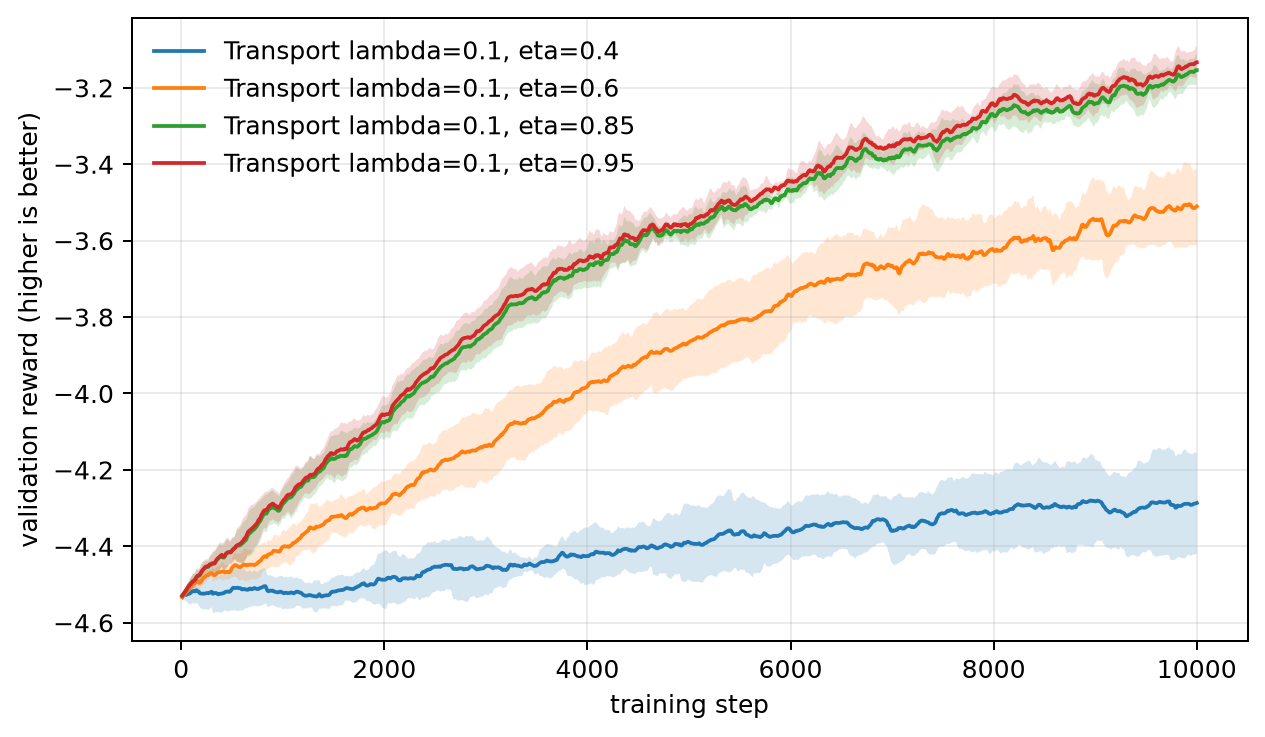
\includegraphics[width=0.49\linewidth]{figures/twostate_eta_sweep_T5.png}
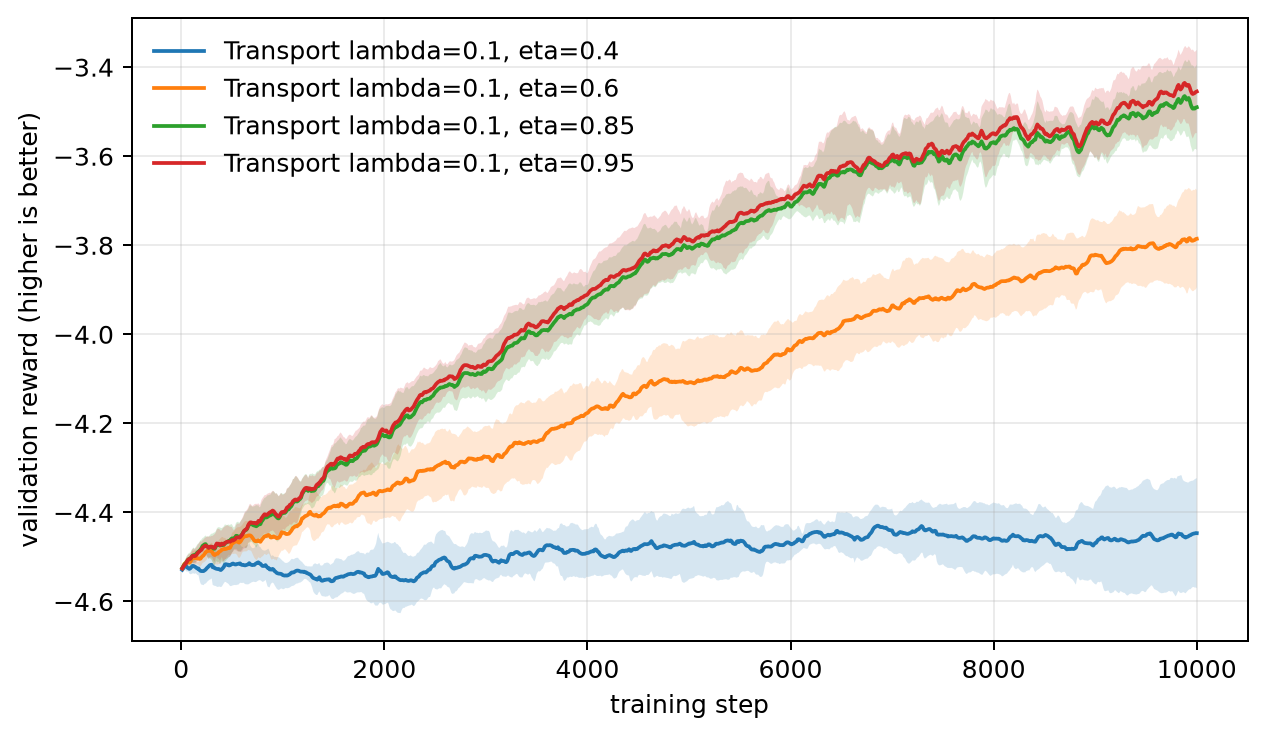
\includegraphics[width=0.49\linewidth]{figures/twostate_eta_sweep_T5_particle.png}
\caption{Two-state benchmark at $T=5$ and $\lambda=0.1$: effect of the auxiliary perturbation scale $\eta$ on the validation reward, as mean over five seeds with one standard deviation shaded, with exact population flow (left) and with a particle approximation of it (right). The ordering in $\eta$ is unchanged by the substitution; the particle runs are uniformly lower and noticeably noisier across seeds.}
\label{fig:twostate-eta}
\end{figure}

\begin{figure}[H]
\centering
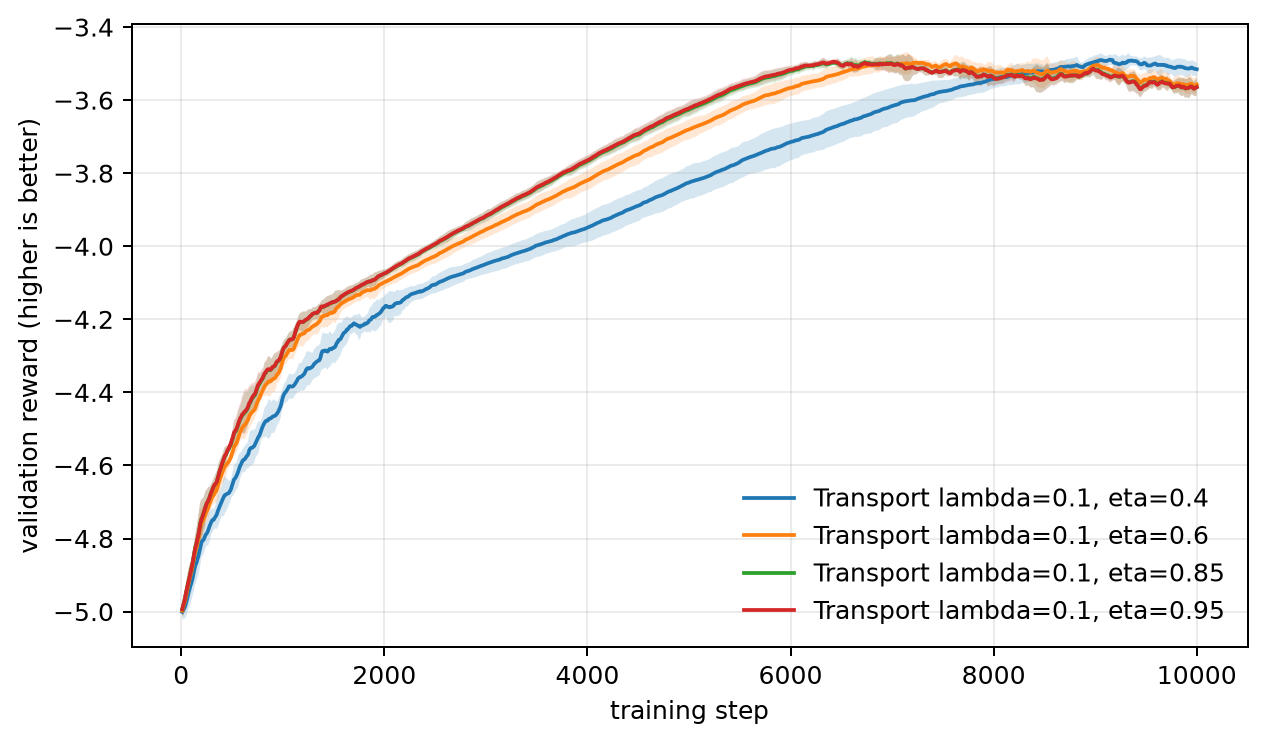
\includegraphics[width=0.49\linewidth]{figures/twostate_eta_sweep_T2.png}
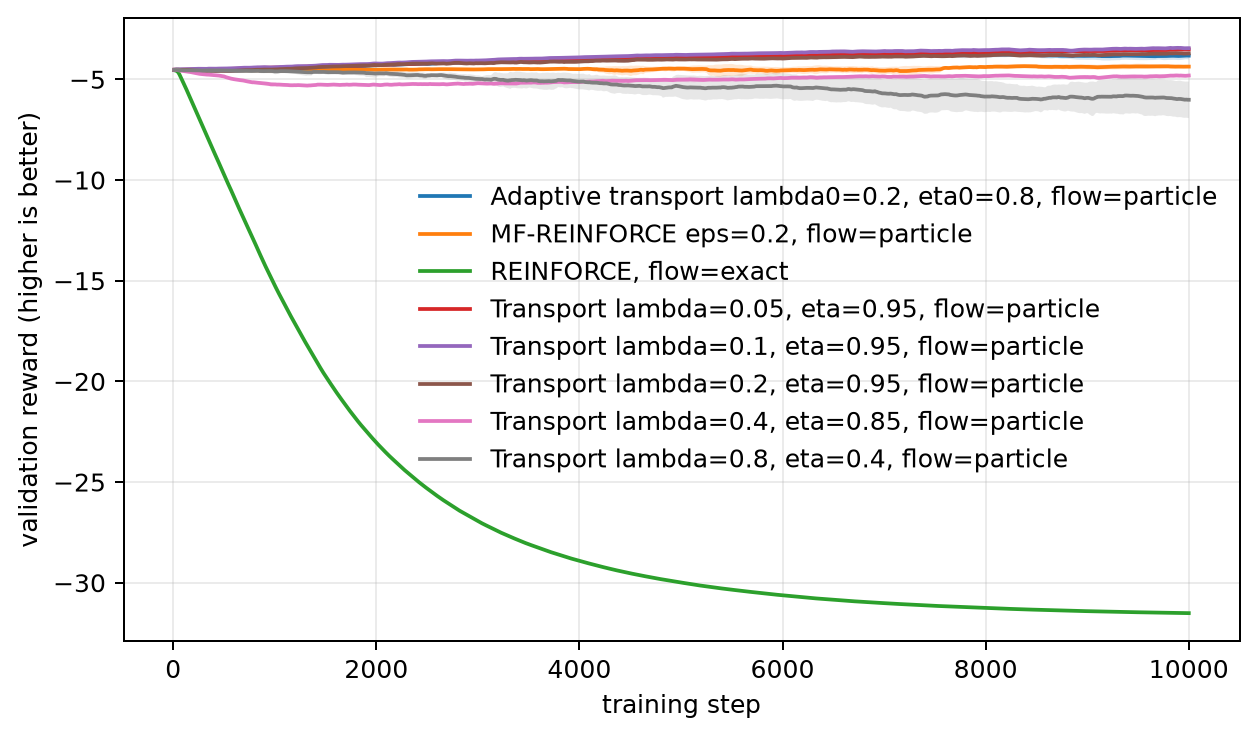
\includegraphics[width=0.49\linewidth]{figures/twostate_validation_T5_particle.png}
\caption{Two-state benchmark. Left: effect of the auxiliary scale $\eta$ at $T=2$ and $\lambda=0.1$, the shorter-horizon counterpart of Figure~\ref{fig:twostate-eta}. Right: validation reward at $T=5$ with a particle approximation of the population flow, to be compared with the exact-flow panel of Figure~\ref{fig:twostate-validation}.}
\label{fig:appendix-twostate}
\end{figure}

\section{Learned flows}
\begin{figure}[H]
\centering
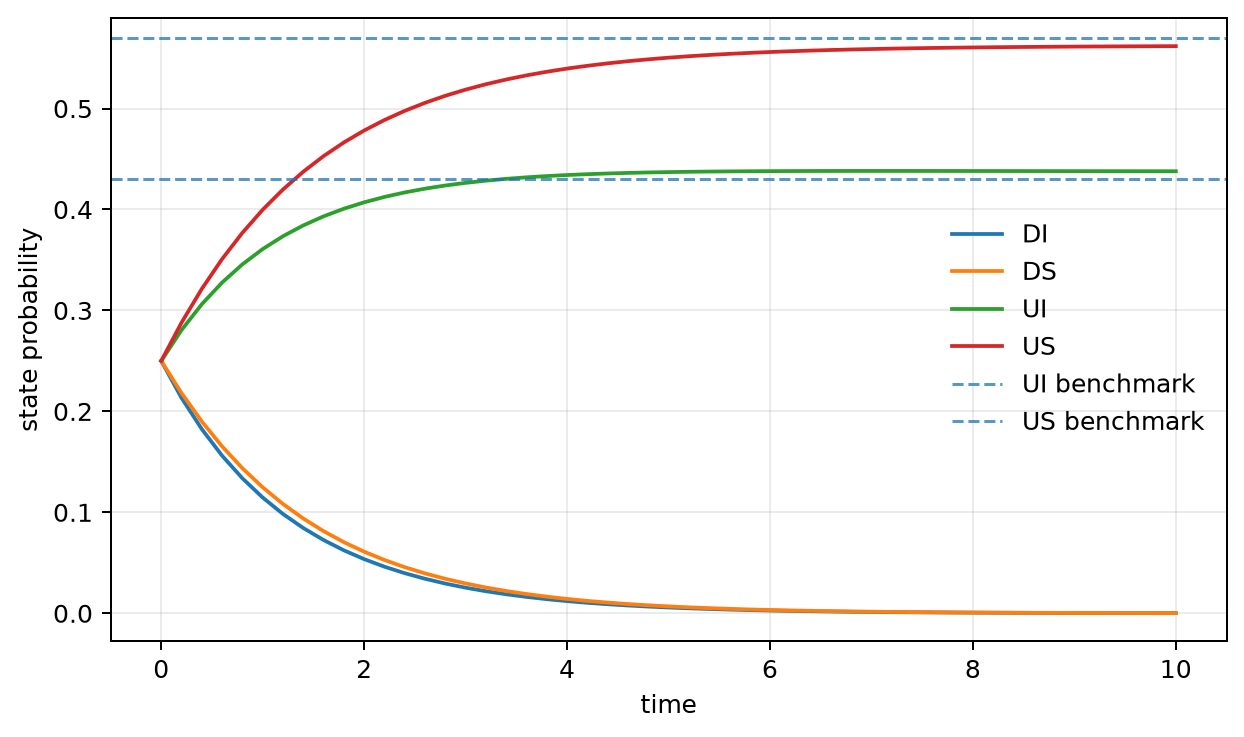
\includegraphics[width=0.49\linewidth]{figures/cyber_flow_reinforce.png}
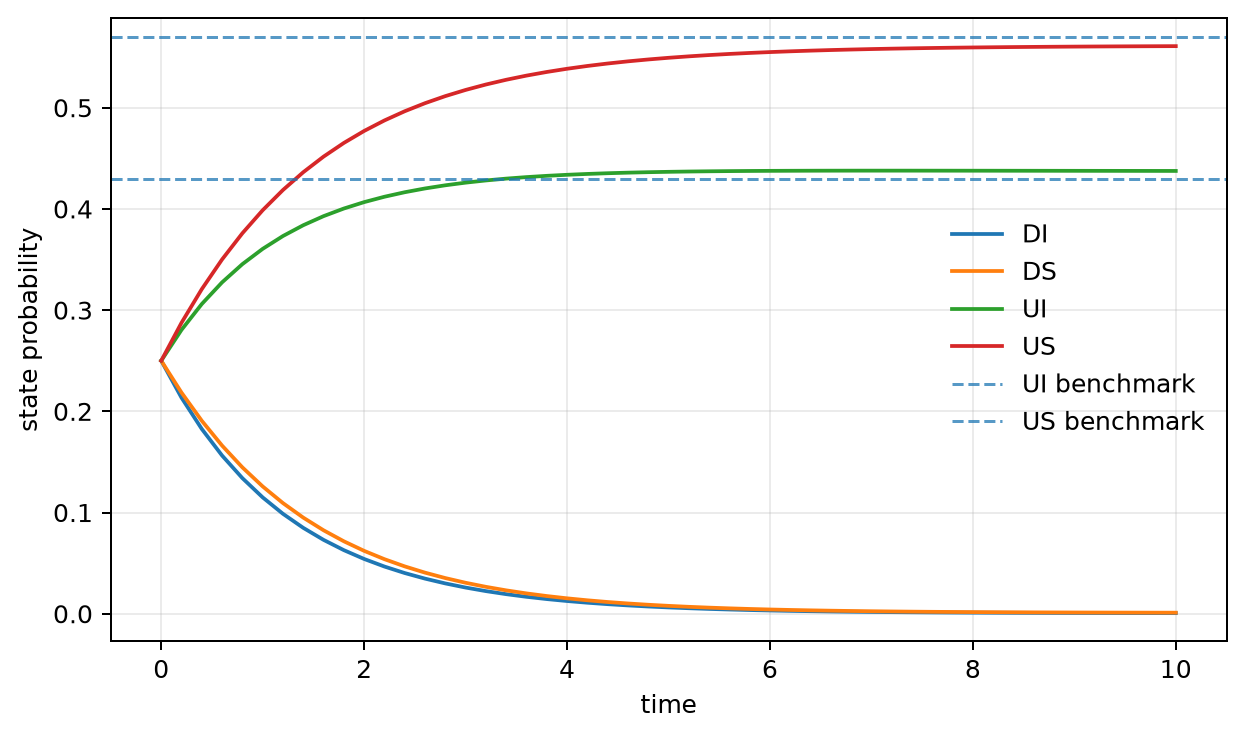
\includegraphics[width=0.49\linewidth]{figures/cyber_flow_mfreinforce.png}
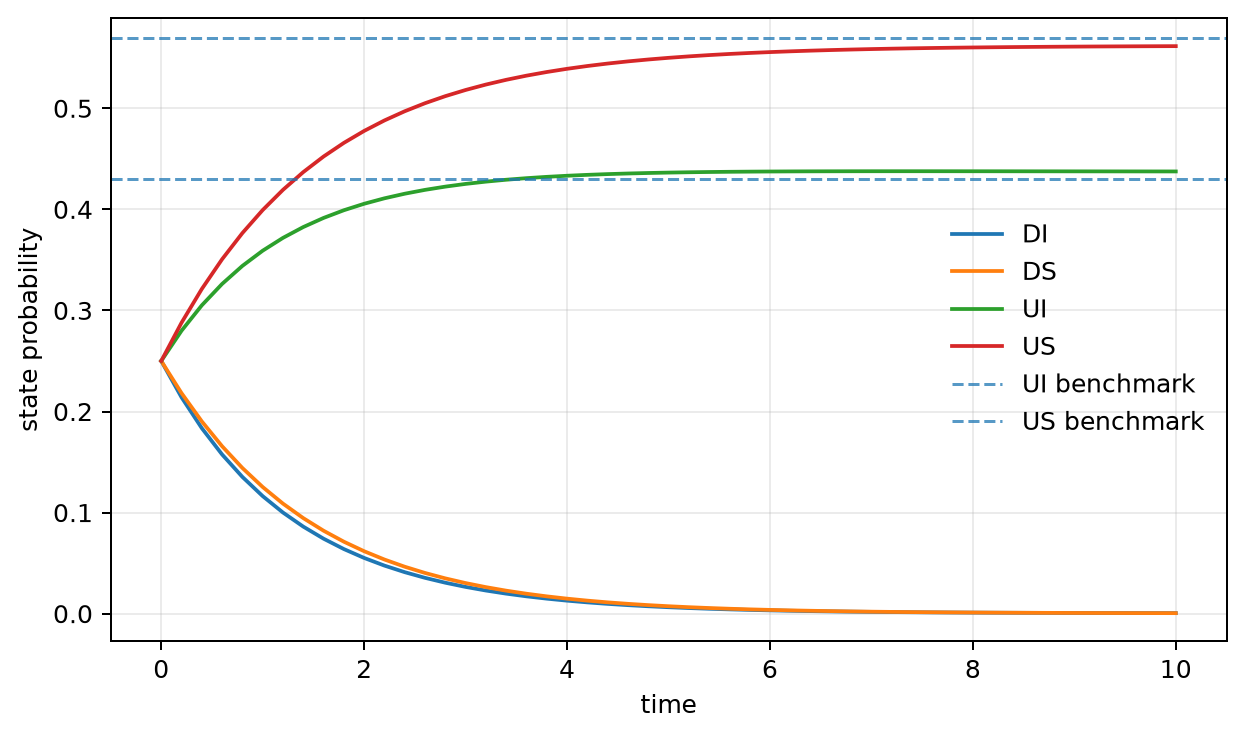
\includegraphics[width=0.49\linewidth]{figures/cyber_flow_transport.png}
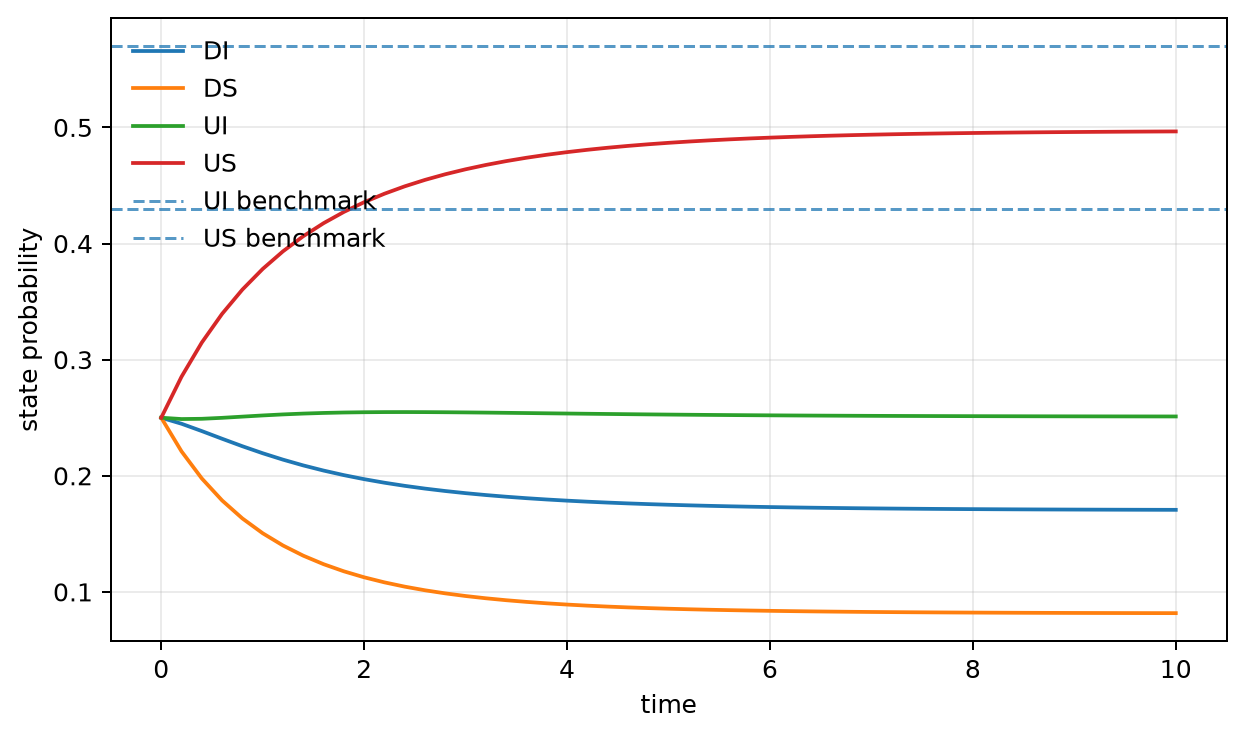
\includegraphics[width=0.49\linewidth]{figures/cyber_flow_adaptive.png}
\caption{Learned state distributions on the cybersecurity benchmark, propagated from the uniform validation law over the full validation episode of $T_{\mathrm{val}}=50$ steps. Top left: REINFORCE. Top right: MF-REINFORCE at $\varepsilon=1$. Bottom left: fixed-scale transport at $\lambda=0.4$. Bottom right: adaptive transport. The dashed lines mark the terminal probabilities of the undefended equilibrium. The first three estimators reach it; the adaptive controller keeps most of the population in the two defended states instead.}
\label{fig:cybersecurity-flows}
\end{figure}

\begin{figure}[H]
\centering
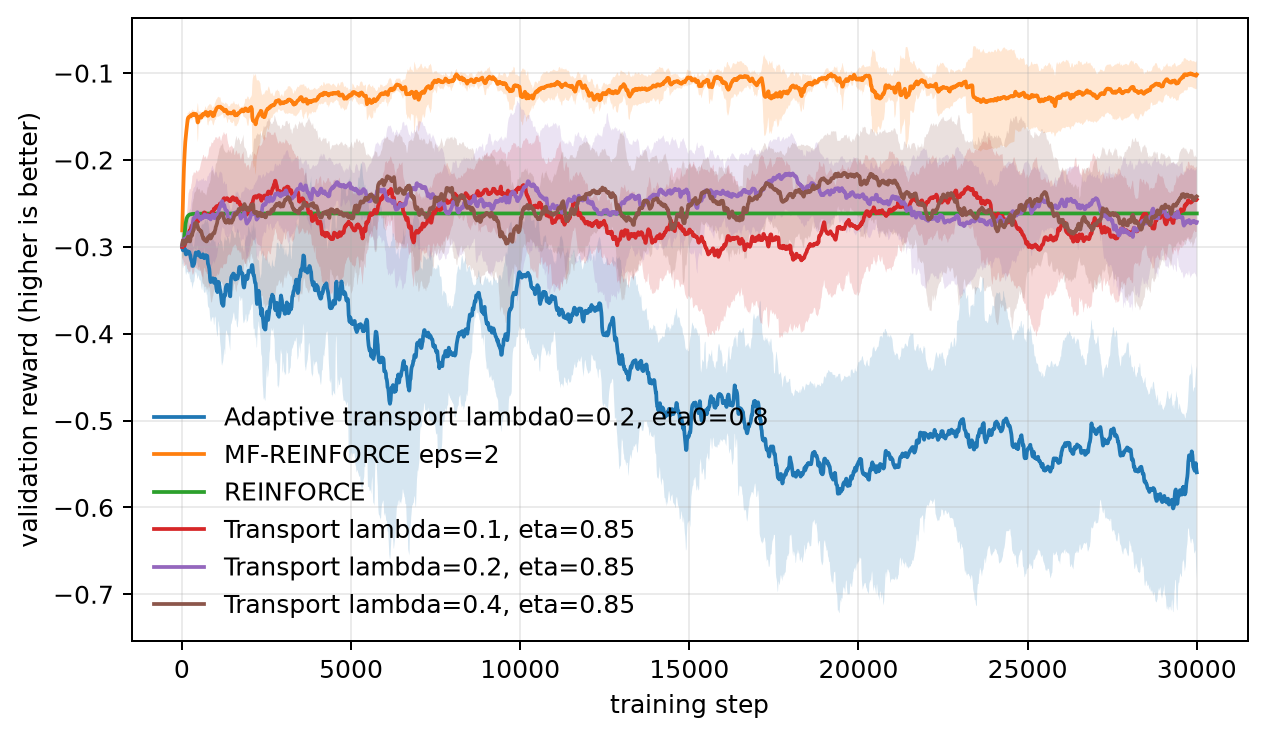
\includegraphics[width=0.62\linewidth]{figures/distribution_validation_T5.png}
\caption{Distribution-planning benchmark at $T=5$: validation reward against training iteration, as mean over five seeds with one standard deviation shaded. REINFORCE is the flat line at $-0.2616$; the transport curves oscillate over tens of thousands of iterations without settling.}
\label{fig:distribution-validation}
\end{figure}

\label{appendix:learned-flows}

Figure~\ref{fig:twostate-flows} compares the population flow learned by all four estimators on the two-state benchmark; the corresponding comparison on cybersecurity, Figure~\ref{fig:cybersecurity-flows}, is kept in the main text because it carries the explanation of that benchmark's ordering. Figure~\ref{fig:appendix-continuous-flows} gives the moment flows on the continuous-state benchmarks.

\begin{figure}[H]
\centering
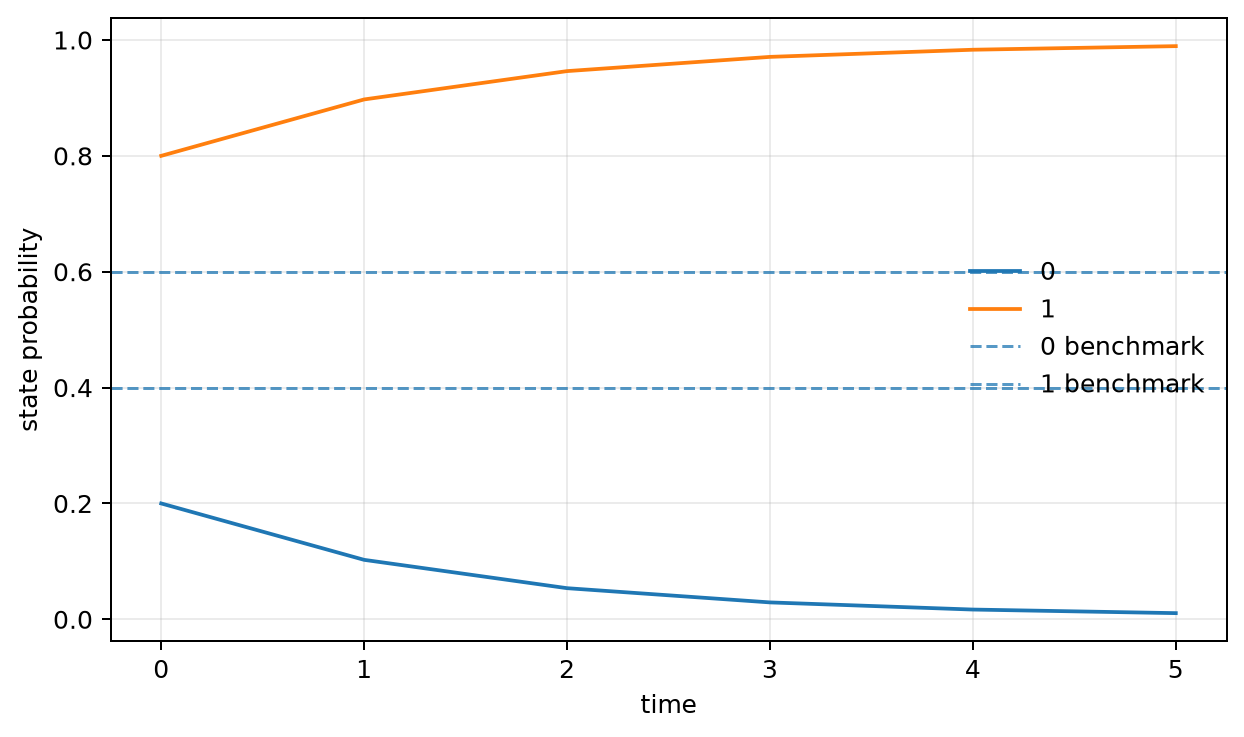
\includegraphics[width=0.49\linewidth]{figures/twostate_flow_reinforce.png}
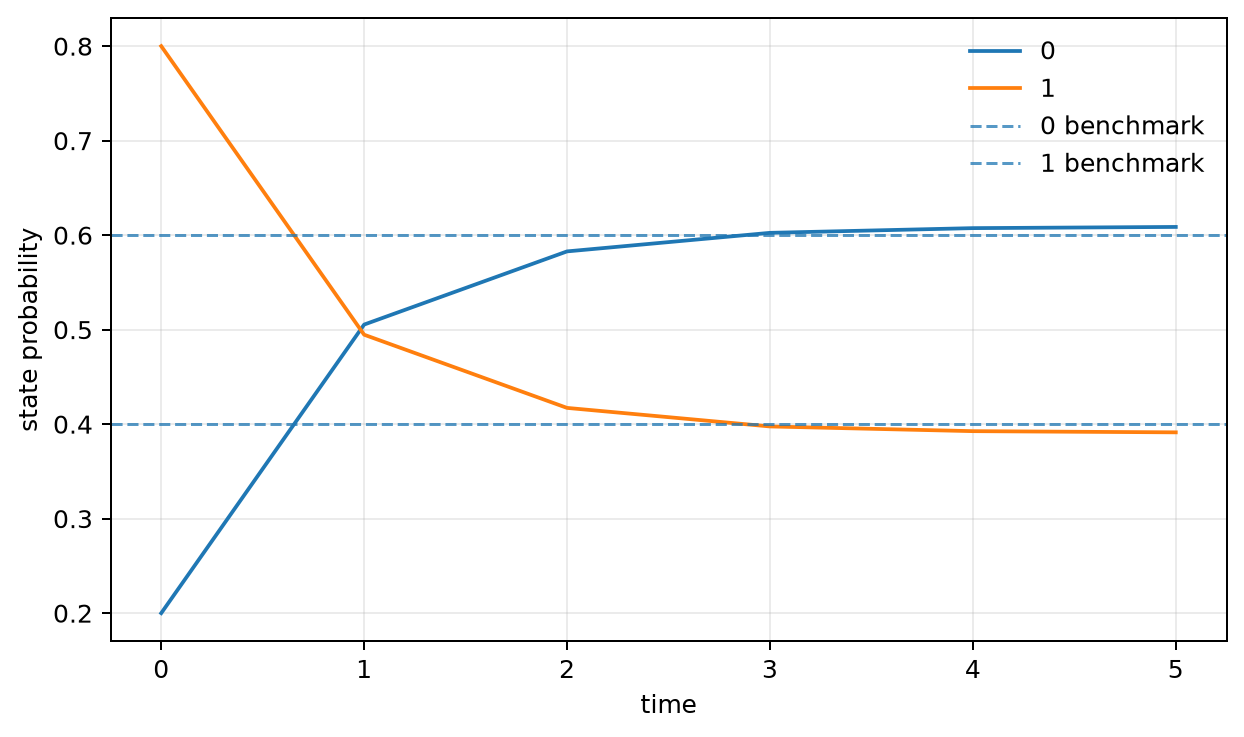
\includegraphics[width=0.49\linewidth]{figures/twostate_flow_mfreinforce.png}
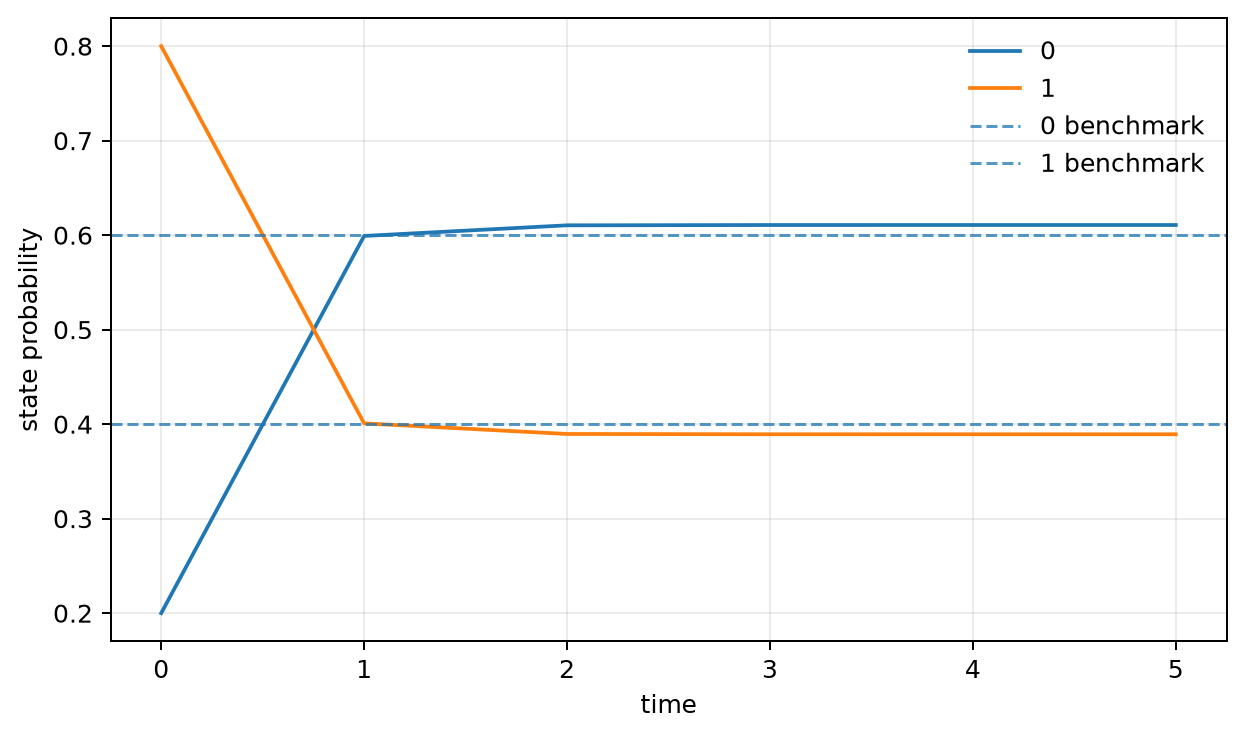
\includegraphics[width=0.49\linewidth]{figures/twostate_flow_transport.png}
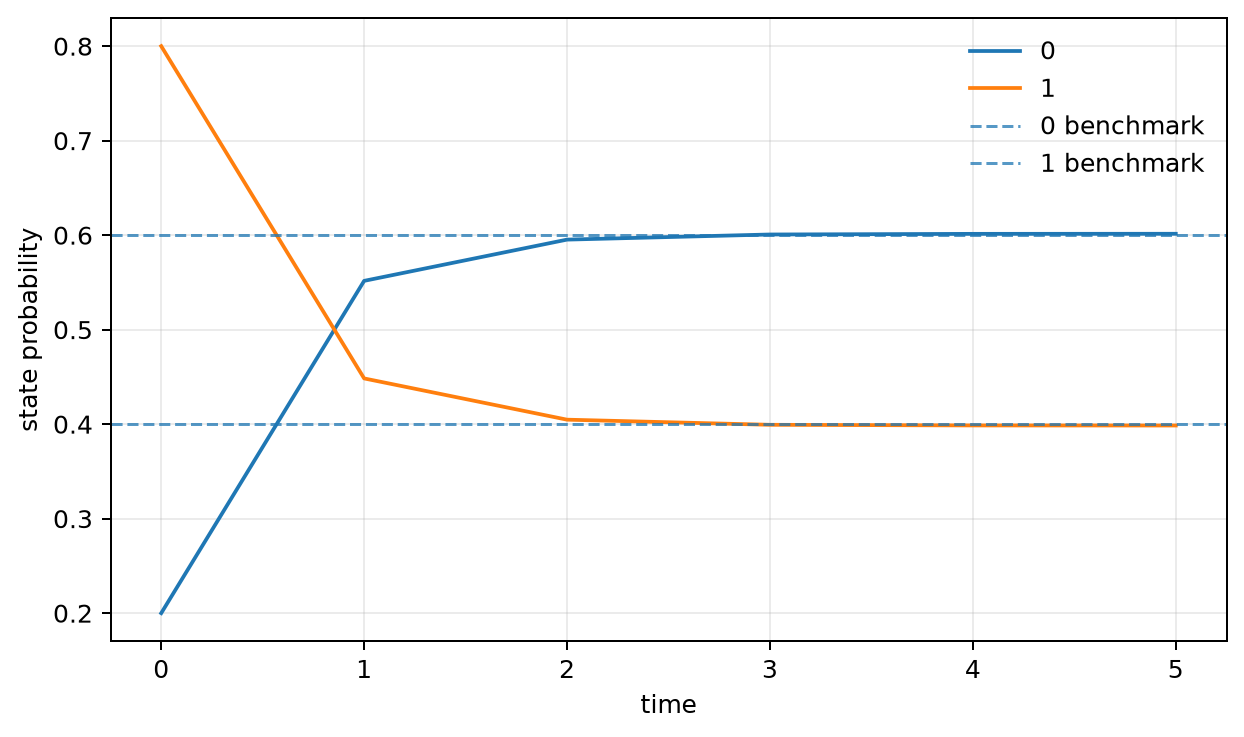
\includegraphics[width=0.49\linewidth]{figures/twostate_flow_adaptive.png}
\caption{Learned population flows on the two-state benchmark at $T=5$ with exact population flow, started from the validation law $\mu_0^{\mathrm{val}}=(0.2,0.8)$. Top left: REINFORCE. Top right: MF-REINFORCE at $\varepsilon=0.2$. Bottom left: fixed-scale transport at $\lambda=0.1$, $\eta=0.95$. Bottom right: adaptive transport. The dashed lines mark the target proportions $(0.6,0.4)$ that the closed-form optimal policy sustains.}
\label{fig:twostate-flows}
\end{figure}

The remaining validation curves follow.

\begin{figure}[H]
\centering
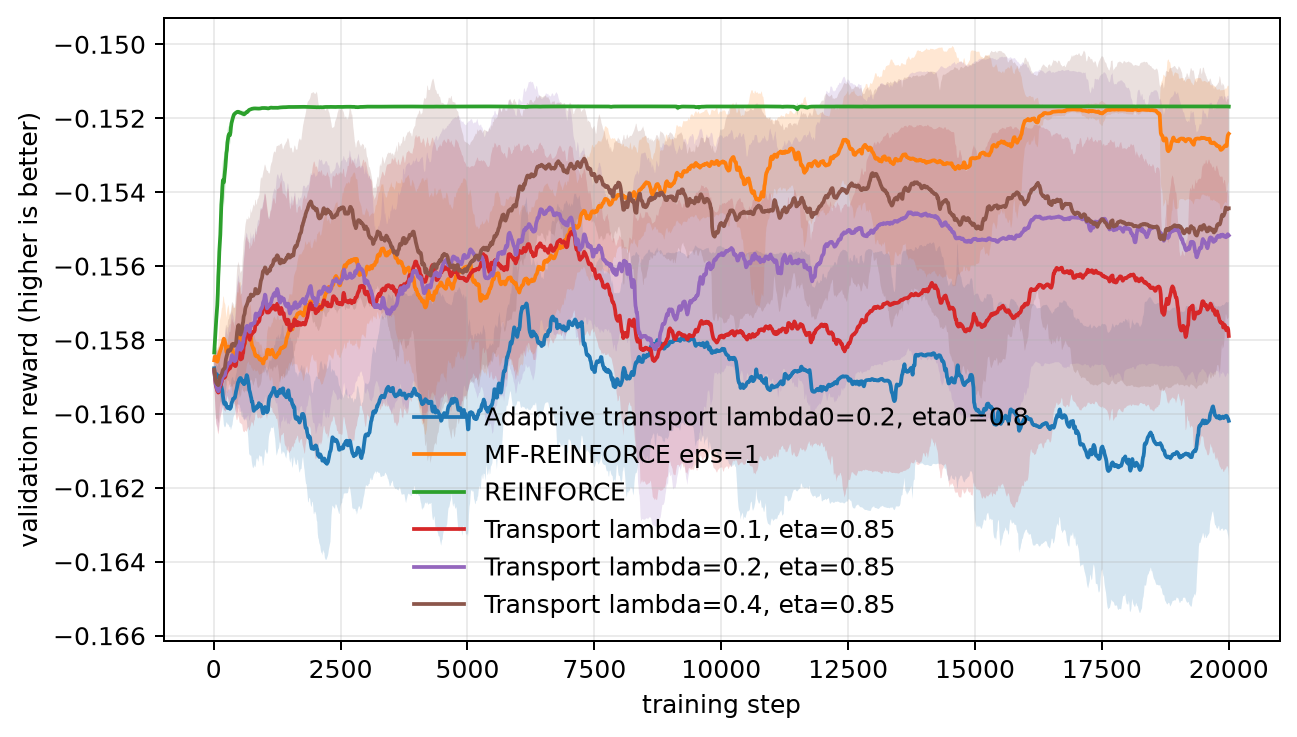
\includegraphics[width=0.68\linewidth]{figures/cybersecurity_validation_T3.png}
\caption{Cybersecurity benchmark at $T=3$: validation reward against training iteration, as mean over five seeds with one standard deviation shaded. REINFORCE converges within a few hundred iterations to the best value in the comparison, and the spread between the best and the worst estimator is under $6\%$ of the objective.}
\label{fig:cybersecurity-validation}
\end{figure}

\begin{figure}[H]
\centering
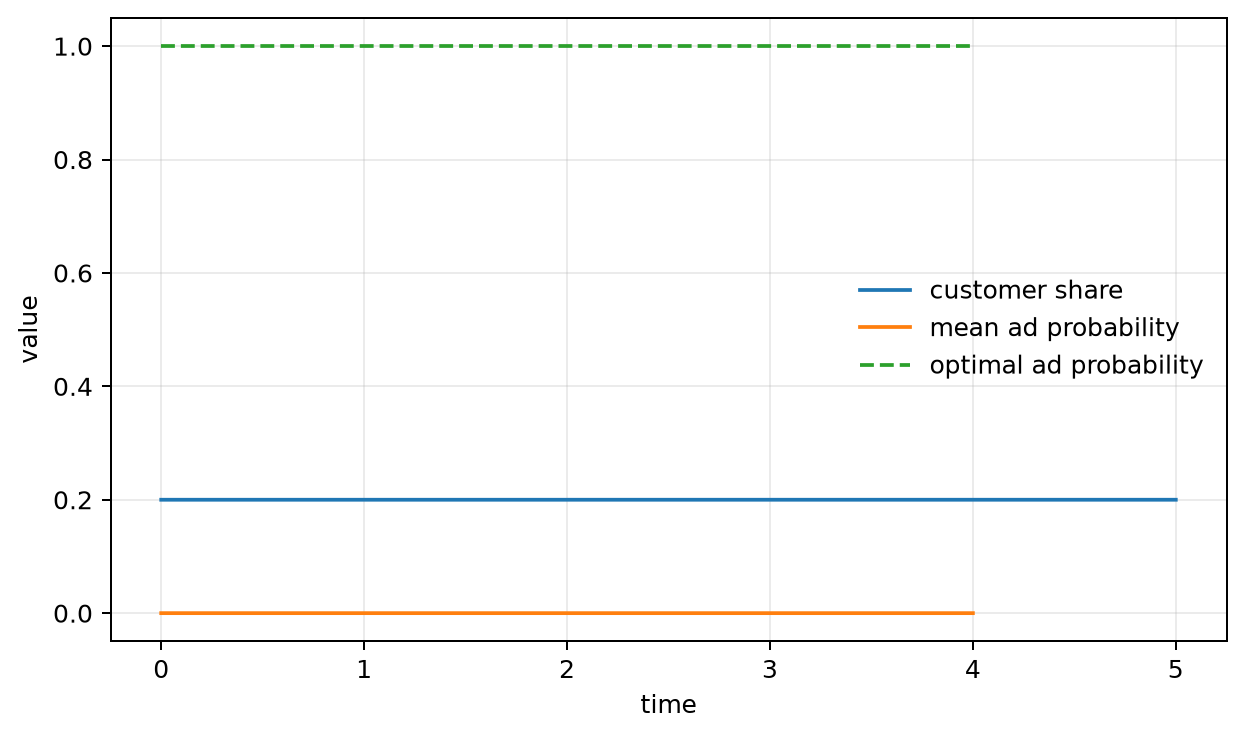
\includegraphics[width=0.32\linewidth]{figures/adv_reinforce.png}
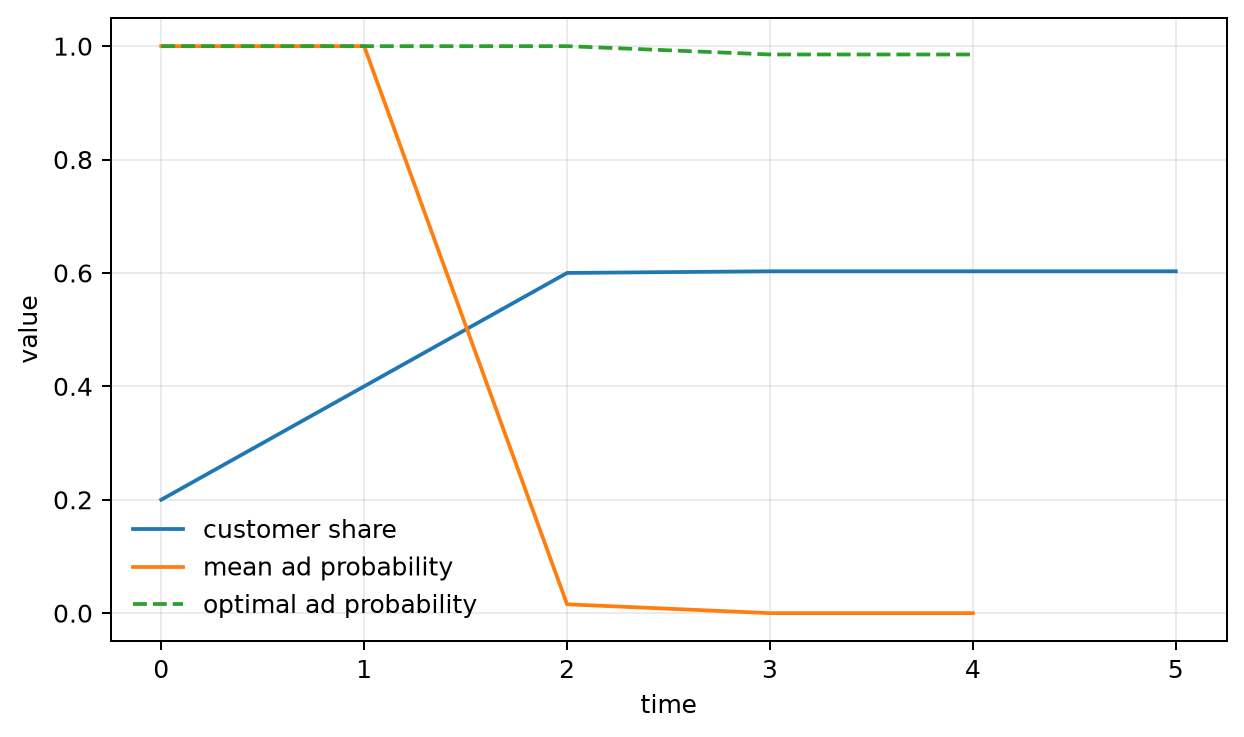
\includegraphics[width=0.32\linewidth]{figures/adv_mfreinforce.png}
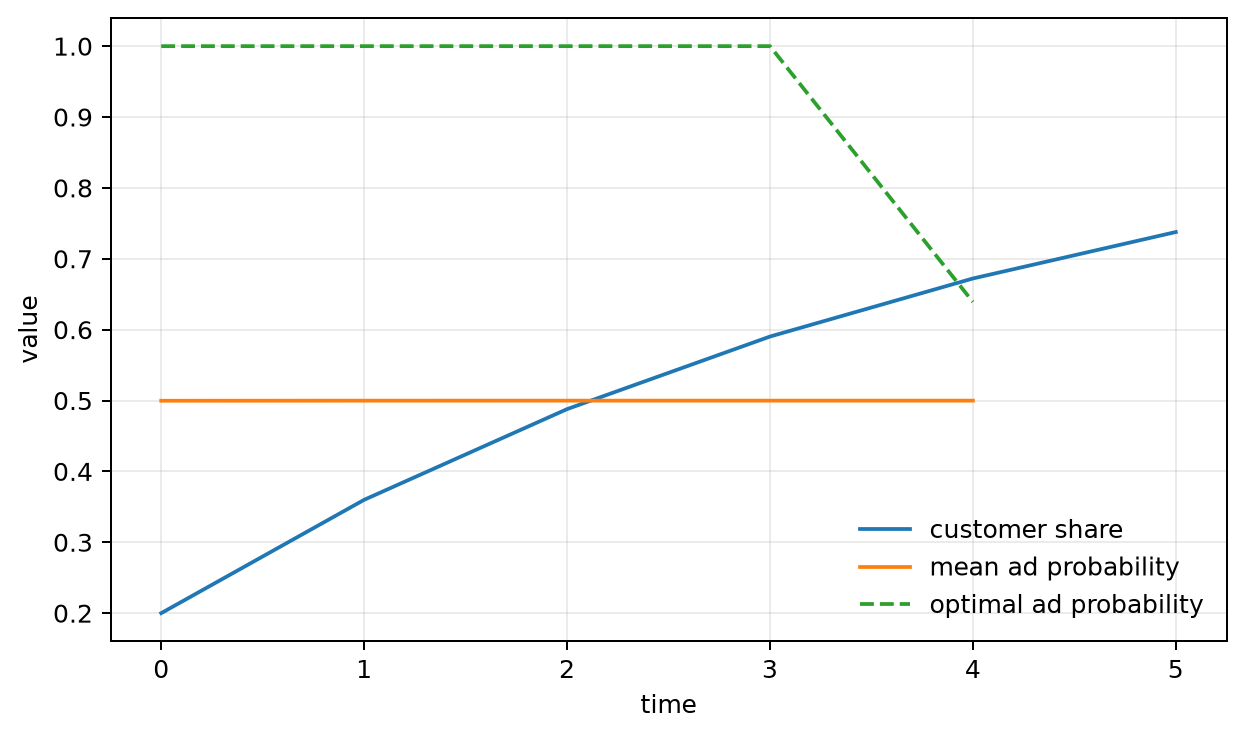
\includegraphics[width=0.32\linewidth]{figures/adv_transport.png}
\caption{Targeted-advertising benchmark at $T=5$: customer share and population-averaged advertising probability of the learned policy against the reference $\widehat q$, for REINFORCE (left), MF-REINFORCE at $\varepsilon=1$ (centre) and fixed-scale transport at $\lambda=0.1$ (right), on the best seed of each. The averaged advertising probability hides a structural difference between the last two, which Table~\ref{tab:advertising-policies} resolves.}
\label{fig:advertising-policy-panels}
\end{figure}

\begin{figure}[H]
\centering
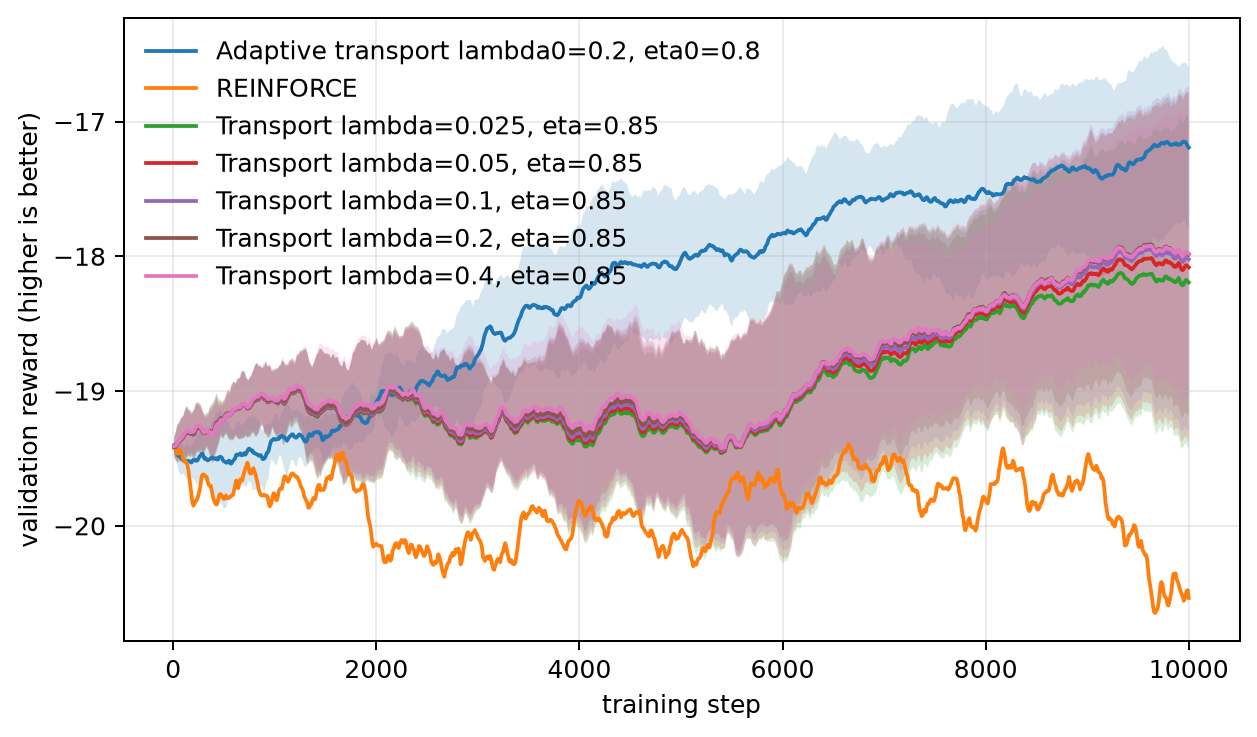
\includegraphics[width=0.68\linewidth]{figures/portfolio_validation_T10.png}
\caption{Mean--variance portfolio benchmark at $T=10$: validation reward against training iteration, as mean over five seeds with one standard deviation shaded. REINFORCE degrades below its initialization; the transport variants improve throughout, and the adaptive controller improves fastest.}
\label{fig:portfolio-validation}
\end{figure}

The figure below gives the moment flows on the continuous-state benchmarks. These are qualitative checks rather than measurements: they verify that the learned policies produce coherent population trajectories rather than the oscillation or collapse that a badly scaled sensitivity estimate would cause.

\begin{figure}[H]
\centering
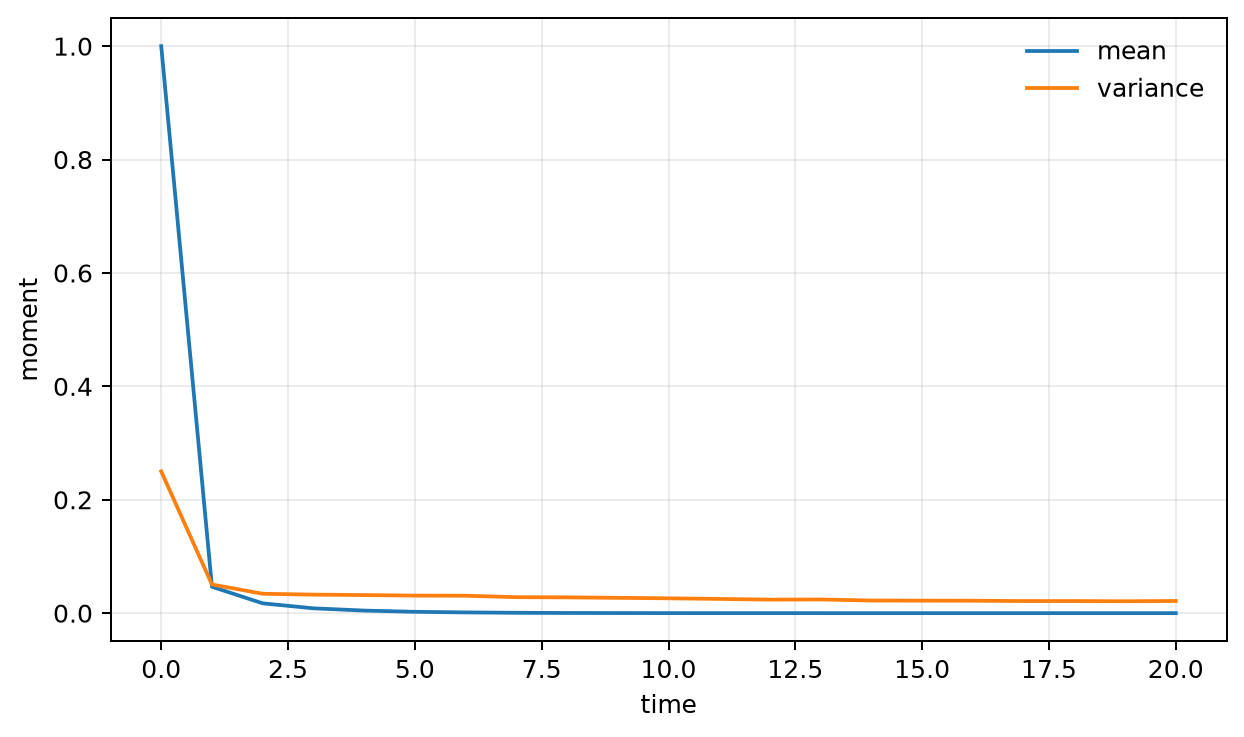
\includegraphics[width=0.46\linewidth]{figures/lq_moment_flow.png}
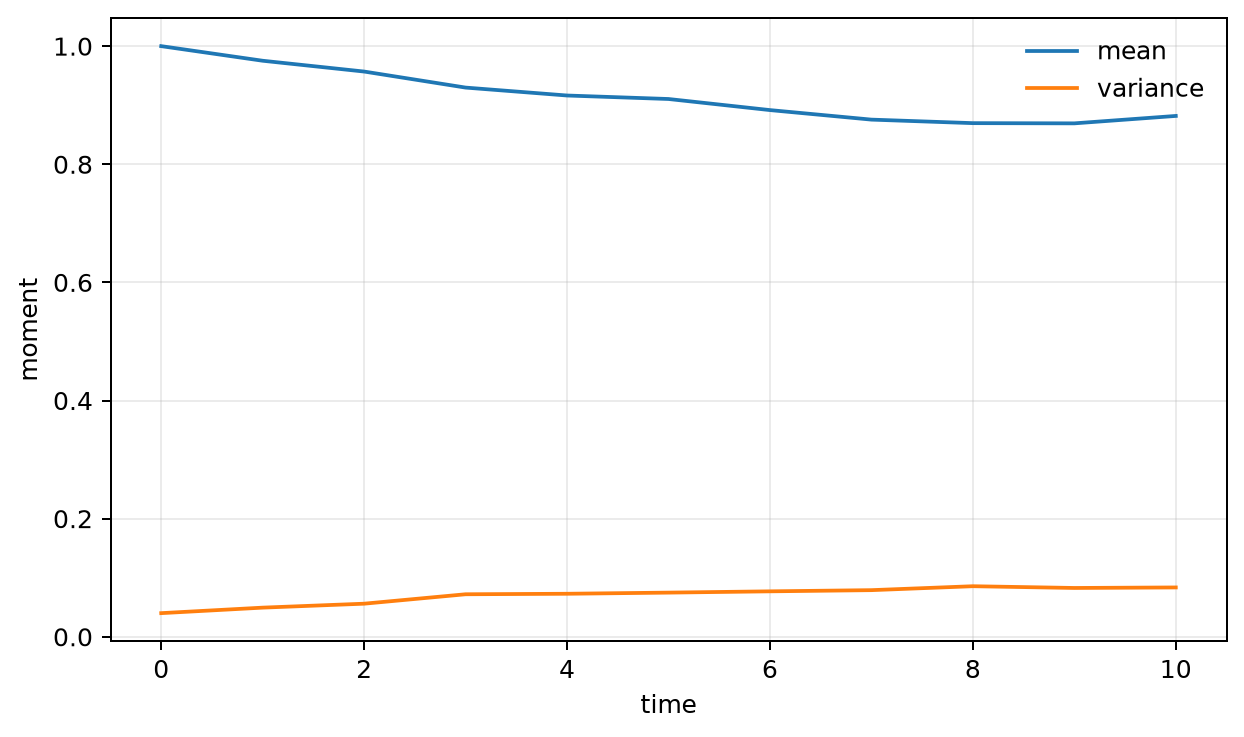
\includegraphics[width=0.46\linewidth]{figures/portfolio_moment_flow.png}
\caption{Learned moment flows on the continuous-state benchmarks, for the best fixed-scale transport configuration of each: linear--quadratic at $T=20$ and $\lambda=0.1$ (left) and portfolio at $T=10$ and $\lambda=0.4$ (right).}
\label{fig:appendix-continuous-flows}
\end{figure}

\section{Population-flow approximation}
\label{appendix:flow-comparison}

\begin{figure}[H]
\centering
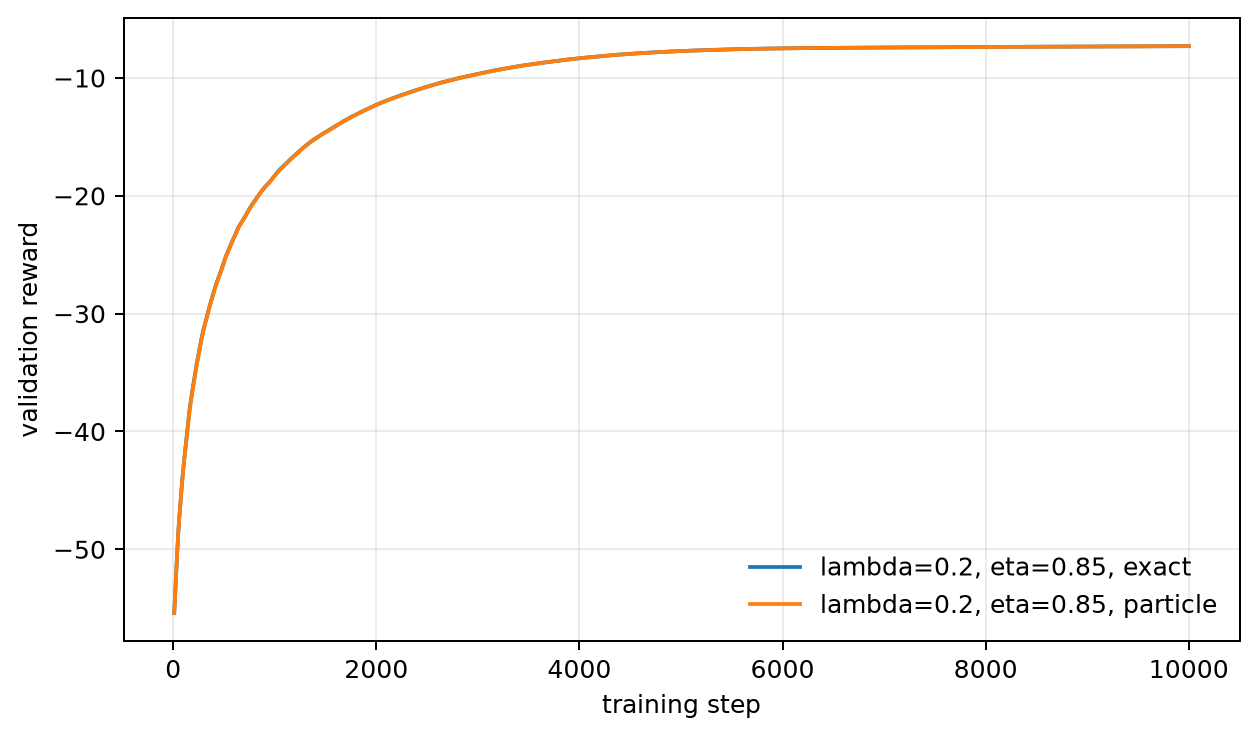
\includegraphics[width=0.62\linewidth]{figures/lq_flow_comparison.png}
\caption{Linear--quadratic benchmark at $T=20$ and $\lambda=0.2$: exact moment recursion against particle estimation of the population flow, as mean over five seeds. The two curves coincide to within the line width.}
\label{fig:lq-flow-comparison}
\end{figure}

Figure~\ref{fig:lq-flow-comparison} compares exact and particle population flow on the linear--quadratic benchmark at $\lambda=0.2$, and Figure~\ref{fig:appendix-flow-comparison} repeats the comparison at the two ends of the perturbation grid. The two flow modes remain indistinguishable at every scale, which is the expected behaviour when the population law enters the dynamics only through its mean.

\begin{figure}[H]
\centering
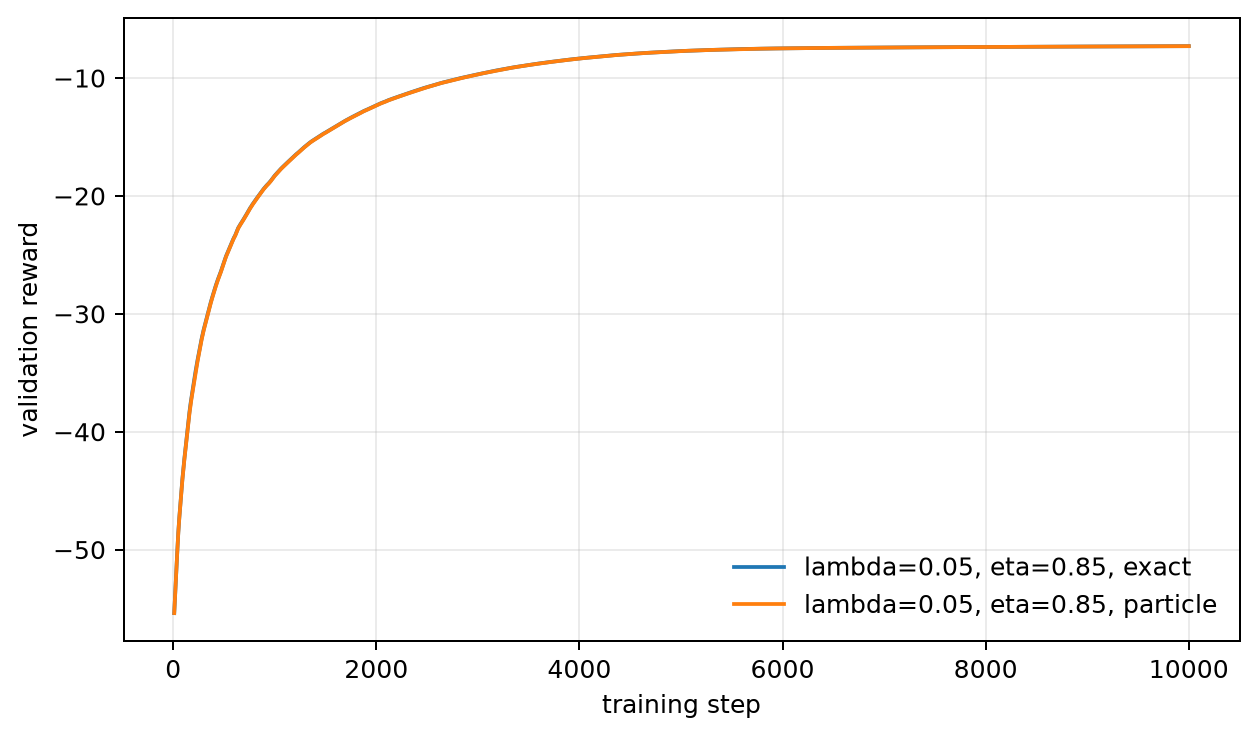
\includegraphics[width=0.49\linewidth]{figures/lq_flow_comparison_l005.png}
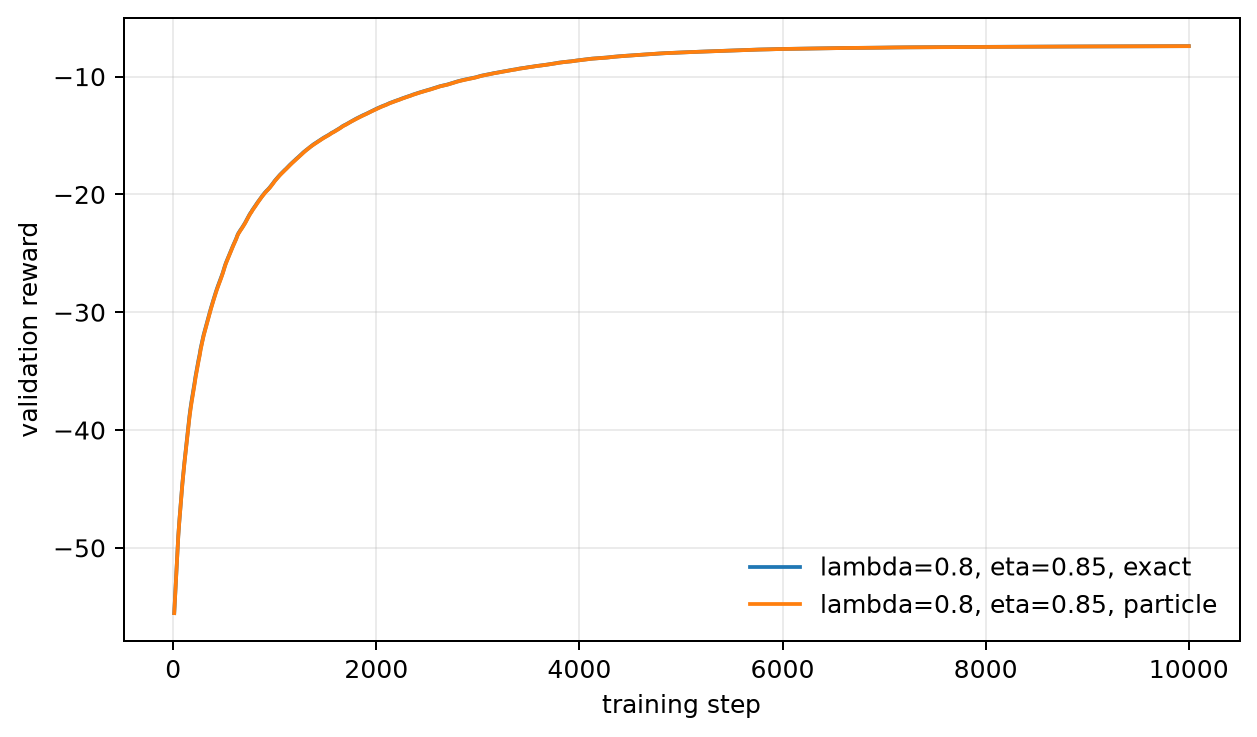
\includegraphics[width=0.49\linewidth]{figures/lq_flow_comparison_l08.png}
\caption{Linear--quadratic benchmark at $T=20$: exact against particle population flow at $\lambda=0.05$ (left) and $\lambda=0.8$ (right), as mean over five seeds.}
\label{fig:appendix-flow-comparison}
\end{figure}

\section{Adaptive schedules}
\label{appendix:adaptive-schedules}

\begin{figure}[H]
\centering
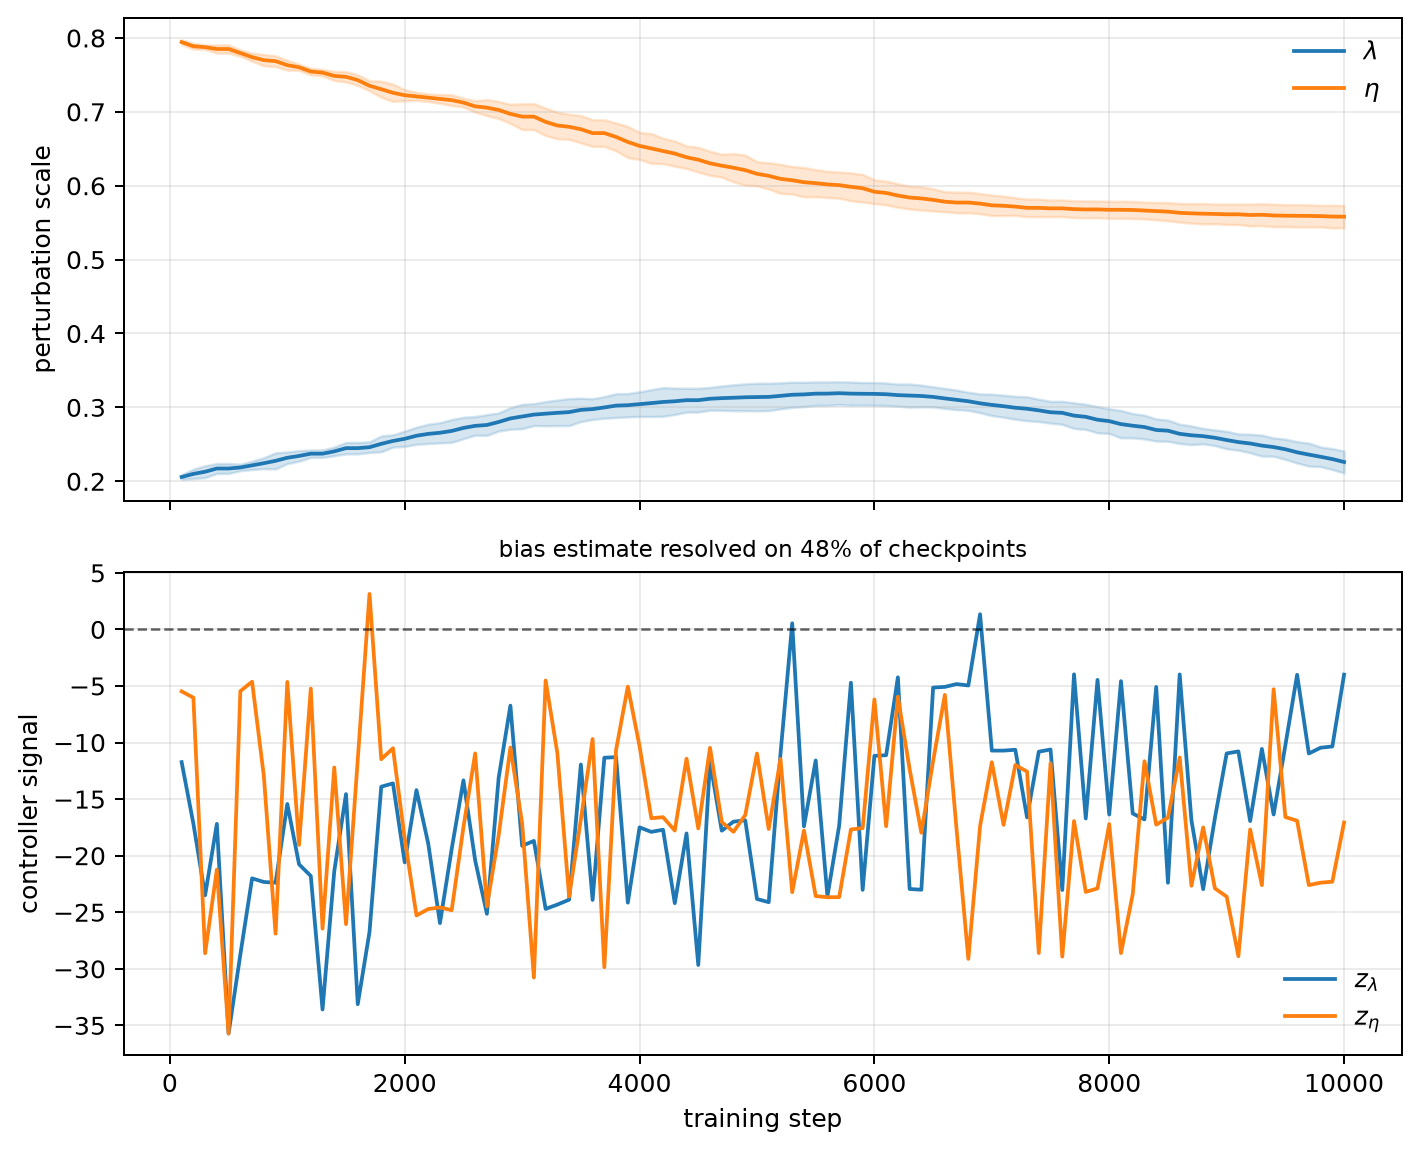
\includegraphics[width=0.62\linewidth]{figures/lq_adaptive_schedule.png}
\caption{Adaptive controller on the linear--quadratic benchmark at $T=20$ with exact population flow. Top: perturbation scales against training iteration, as mean over five seeds with one standard deviation shaded. Bottom: the logarithmic balance signals $z_\lambda$ and $z_\eta$, negative almost everywhere, indicating a variance-dominated regime.}
\label{fig:adaptive-schedule}
\end{figure}

Figure~\ref{fig:adaptive-schedule} shows the controller trajectory on the linear--quadratic benchmark. Figure~\ref{fig:appendix-adaptive} gives the two benchmarks on which the controller underperforms the fixed grid. Both contract the main scale to the bottom of its range, and the contrast with the linear--quadratic trajectory, which is non-monotone in $\lambda$ and settles an order of magnitude higher, is the observation discussed in Section~\ref{sec:adaptive-control}.

\begin{figure}[H]
\centering
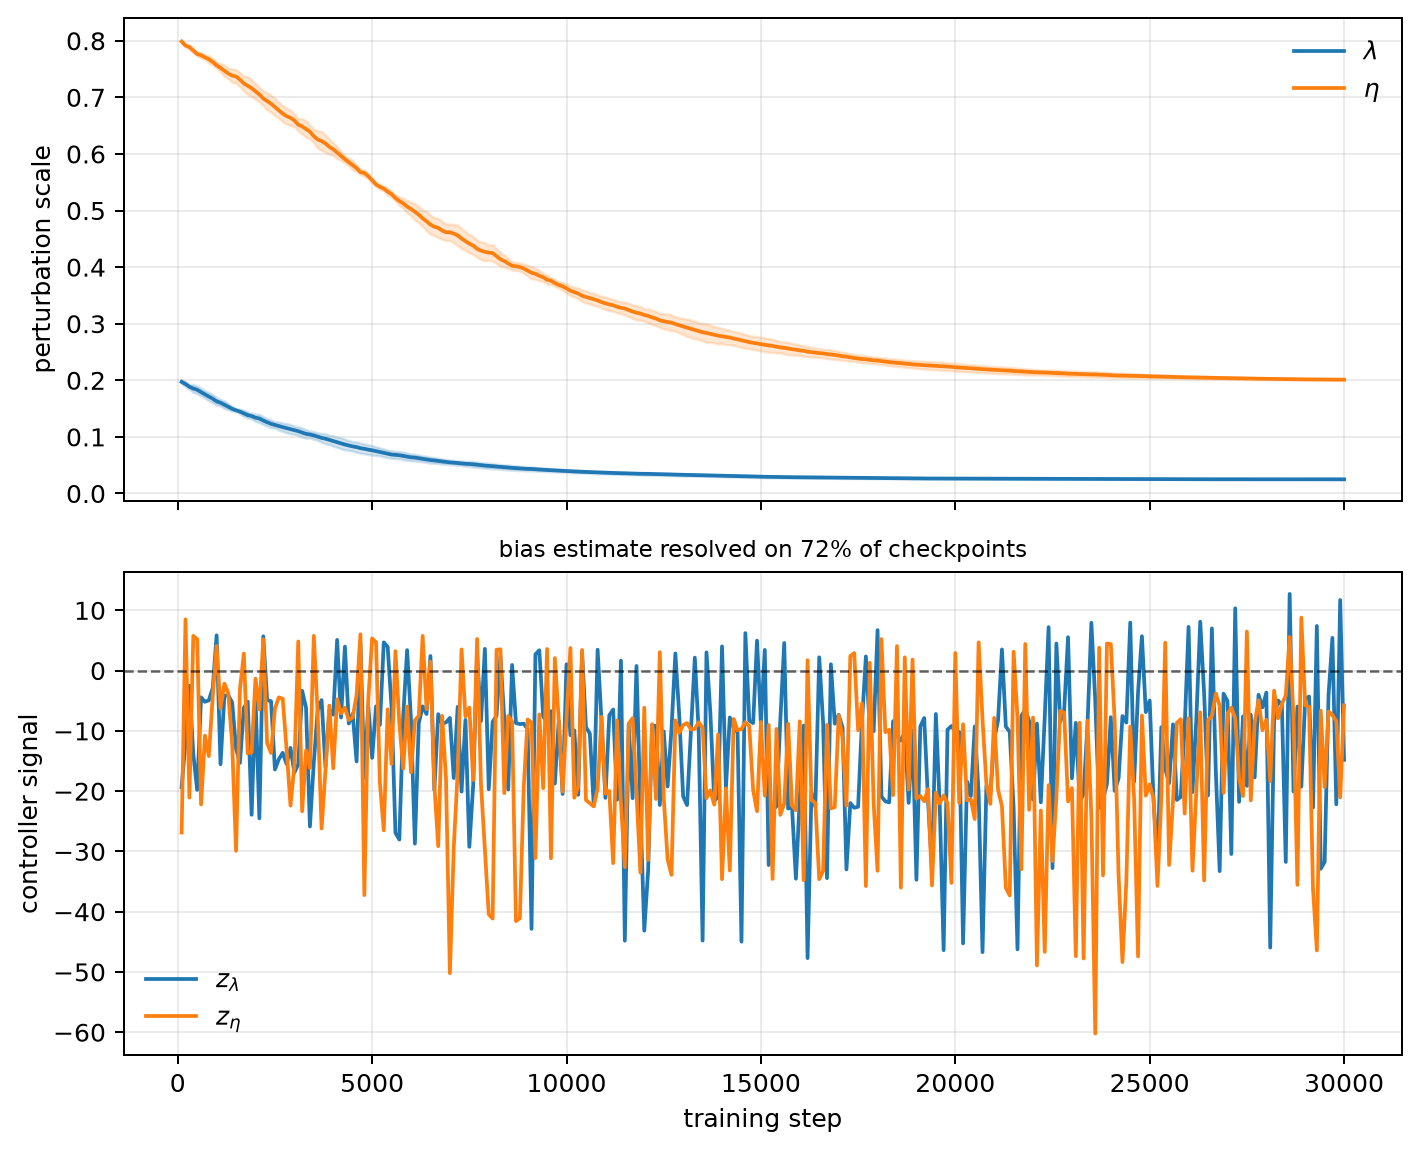
\includegraphics[width=0.49\linewidth]{figures/distribution_adaptive_schedule.png}
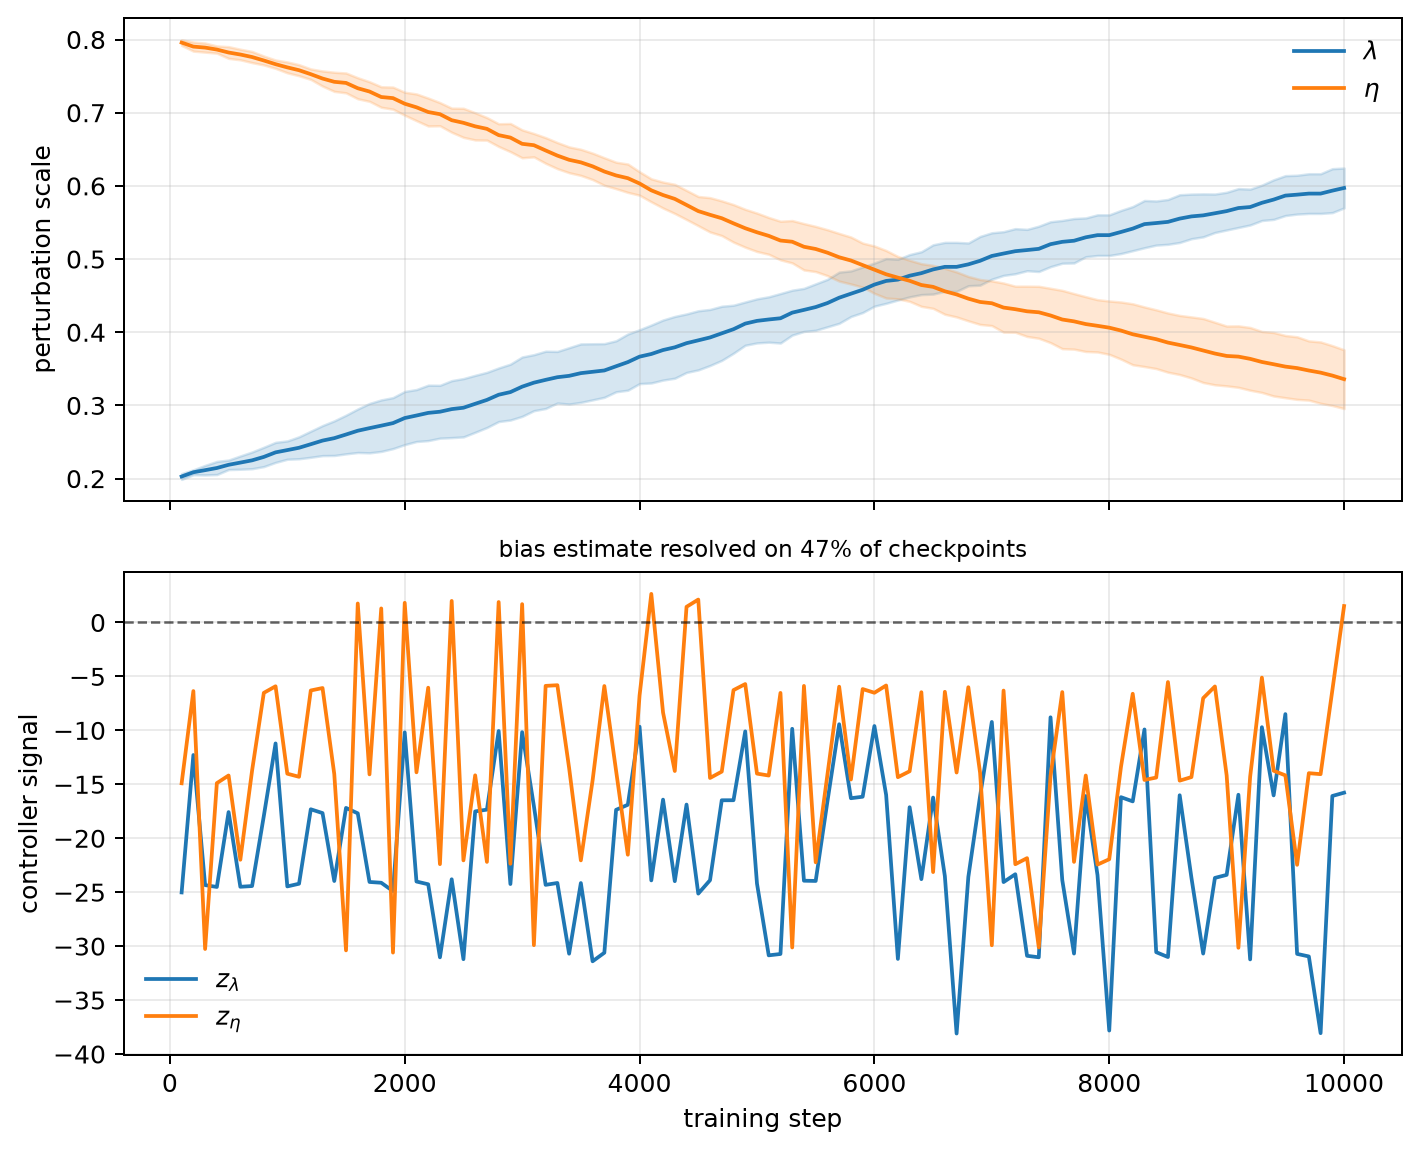
\includegraphics[width=0.49\linewidth]{figures/portfolio_adaptive_schedule.png}
\caption{Adaptive controller on distribution planning at $T=5$ (left) and on the portfolio benchmark at $T=10$ (right). Top panels: perturbation scales against training iteration, as mean over five seeds with one standard deviation shaded. Bottom panels: the logarithmic balance signals $z_\lambda$ and $z_\eta$.}
\label{fig:appendix-adaptive}
\end{figure}

\section{Allocating the auxiliary budget}
\label{appendix:auxiliary-budget}

The equal-budget rule of Section~\ref{subsec:experimentation-protocol} fixes the total number of simulated transitions per update, $T(B_{\mathrm{tr}}+n_{\mathrm{tr}})$, but not its split between the main trajectories and the auxiliary sensitivity estimate. Table~\ref{tab:auxiliary-budget} records that split on every benchmark, together with the number $d$ of free coordinates of the population argument that the auxiliary estimate has to resolve.

\begin{table}[H]
\centering
\begin{tabular}{llrrrrr}
\toprule
Benchmark & Argument & $d$ & $B_{\mathrm{tr}}$ & $n_{\mathrm{tr}}$ & $n_{\mathrm{tr}}/d$ & Budget \\
\midrule
Two-state & $\Delta_2$ & 1 & 248 & 12 & $12.0$ & $1\,300$ \\
Cybersecurity & $\Delta_4$ & 3 & 184 & 20 & $6.7$ & $612$ \\
Distribution planning & $\Delta_{10}$ & 9 & 549 & 11 & $1.2$ & $2\,800$ \\
Targeted advertising & $\Delta_2$ & 1 & 248 & 12 & $12.0$ & $1\,300$ \\
Linear--quadratic & mean & 1 & 201 & 20 & $20.0$ & $4\,420$ \\
Portfolio & mean & 1 & 311 & 200 & $200.0$ & $5\,110$ \\
\bottomrule
\end{tabular}
\caption{Split of the matched simulator budget between the main trajectories $B_{\mathrm{tr}}$ and the auxiliary sensitivity trajectories $n_{\mathrm{tr}}$ of the fixed-scale transport estimator, with $d$ the number of free coordinates of the population argument. The equal-budget rule constrains $T(B_{\mathrm{tr}}+n_{\mathrm{tr}})$ but not the split, which was reallocated towards the auxiliary estimate on the continuous-state benchmarks and left at the default on the finite-state ones. The resulting auxiliary sample size per coordinate spans more than two orders of magnitude, and distribution planning is the one benchmark where it falls close to one.}
\label{tab:auxiliary-budget}
\end{table}


The ratio $n_{\mathrm{tr}}/d$ spans more than two orders of magnitude across the suite, and distribution planning is the extreme case. Its transport runs use $B_{\mathrm{tr}}=549$ main and $n_{\mathrm{tr}}=11$ auxiliary trajectories against a ten-point simplex with $d=9$, that is $1.2$ auxiliary trajectories per coordinate, against $6.7$ on cybersecurity, $12$ on the two-state and advertising problems, $20$ on the linear--quadratic benchmark and $200$ on the portfolio benchmark. It is the only benchmark on which the auxiliary estimate is asked to resolve more coordinates than it has samples, and the only finite-state benchmark on which transport loses to MF-REINFORCE by a wide margin. Whether that association is causal is the question taken up as an extension in Section~\ref{sec:extensions}. This section records the two measurements bearing on it: what a reallocation costs, and what it does on a benchmark where the hypothesis predicts nothing.

\paragraph{The cost of reallocating.}
The split can be changed without changing the budget, since the rule constrains only the sum: on distribution planning, taking $B_{\mathrm{tr}}=200$ and $n_{\mathrm{tr}}=360$ leaves $T(B_{\mathrm{tr}}+n_{\mathrm{tr}})=2\,800$ unchanged and raises the auxiliary sample size to $40$ per coordinate. It is also affordable in arithmetic. One might expect the cost of the update to grow linearly in $n_{\mathrm{tr}}$, but the sensitivity recursion is applied to the whole auxiliary batch at once, and a direct measurement gives a factor $1.9$ in seconds per training step when $n_{\mathrm{tr}}$ goes from $11$ to $360$, a $33$-fold increase in auxiliary samples. The dominant cost of the update on this benchmark is the exact population recursion over the ten-point simplex, which the reallocation does not touch. Applied to a base cost of $6\,802$ seconds per transport seed over $30\,000$ iterations (Table~\ref{tab:budget-runtime}), that factor nonetheless puts a five-seed reallocated arm outside the compute budget of the internship so far, which is why the experiment is proposed in Section~\ref{sec:extensions} rather than reported here.

\paragraph{A negative control on targeted advertising.}
Table~\ref{tab:reallocation} reports the same reallocation on a benchmark where the hypothesis predicts no effect. The advertising population argument is a two-point simplex with a single free coordinate, and its transport runs already use $n_{\mathrm{tr}}=12$ auxiliary trajectories, the same ratio as the two-state benchmark on which transport is the best estimator at $T=5$. Moving the split from $(B_{\mathrm{tr}},n_{\mathrm{tr}})=(248,12)$ to $(100,160)$ at fixed budget takes the final objective from $0.9795\pm0.0089$ to $0.9734\pm0.0079$, a difference well inside one standard deviation. Where the auxiliary estimate is already resolved, moving budget towards it does not help, which is what the hypothesis predicts; Section~\ref{subsec:targeted-advertising} identifies a different mechanism as the limitation there. The control establishes the absence of an effect where the ratio is already high; the positive arm is what the extension of Section~\ref{sec:extensions} would supply.

\begin{table}[H]
\centering
\small
\begin{tabular}{llrrrrrr}
\toprule
Benchmark & $\lambda$ & $B_{\mathrm{tr}}$ & $n_{\mathrm{tr}}$ & $n_{\mathrm{tr}}/d$ & Iterations & Objective & Seeds \\
\midrule
Targeted advertising & $0.1$ & 248 & 12 & $12.0$ & $10\,000$ & $0.9795\pm0.0089$ & 5 \\
 &  & 100 & 160 & $160.0$ &  & $0.9734\pm0.0079$ & 5 \\
\bottomrule
\end{tabular}
\caption{Recorded check of moving the matched simulator budget from the main trajectories towards the auxiliary sensitivity estimate. Both rows use the same estimator, perturbation scales, simulator budget $T(B_{\mathrm{tr}}+n_{\mathrm{tr}})$ and number of training iterations; only the split differs. The table compares the two allocations at the iteration count given in the sixth column, reading the default arm from its recorded validation history at the same point, and reports the mean and standard deviation over the seeds indicated. Higher is better.}
\label{tab:reallocation}
\end{table}


\section{Perturbation bound along the learned flows}
\label{appendix:theory-tables}
\label{appendix:tv-bounds}

Table~\ref{tab:tv-bounds} is the first of the measurement tables behind Table~\ref{tab:theory-verdicts} of Section~\ref{sec:theory-validation}, recording the largest value of $d_{\mathrm{TV}}(M_t^{\lambda,\theta},\mu_t^\theta)/\lambda$ along the learned flow of every finite-state transport run. The other two, the objective bias against the perturbation scale and the replicated gradient diagnostics, are reported in the body of that section.

\begin{table}[H]
\centering
\begin{tabular}{lrrrr}
\toprule
Benchmark & Configurations & Measured points & $\max_t d_{\mathrm{TV}}/\lambda$ & Satisfies $d_{\mathrm{TV}}\leq\lambda$ \\
\midrule
Two-state & 80 & 400 & $0.800$ & 400/400 \\
Cybersecurity & 3 & 15 & $0.843$ & 15/15 \\
Distribution planning & 3 & 15 & $1.000$ & 15/15 \\
Targeted advertising & 3 & 15 & $0.800$ & 15/15 \\
\midrule
Total & $89$ & $445$ & & 445/445 \\
\bottomrule
\end{tabular}
\caption{Perturbation bound on the finite-state benchmarks. For every transport run the largest value of $d_{\mathrm{TV}}(M_t^{\lambda,\theta},\mu_t^\theta)$ along the learned population flow is compared with $\lambda$. The bound holds at every measured point, and is attained to within a factor $d_{\mathrm{TV}}(q_t,\mu_t^\theta)\leq1$ of $\lambda$, so the perturbation is neither degenerate nor larger than the theory allows.}
\label{tab:tv-bounds}
\end{table}


\section{The population-dependence ablation}
\label{appendix:gamma-ablation}

Table~\ref{tab:correction-alignment-ablation} is the controlled pair discussed in Section~\ref{sec:correction-alignment}.

\begin{table}[H]
\centering
\begin{tabular}{llrrrl}
\toprule
Benchmark & Setting & $\|G_{\mathrm{full}}\|$ & $\|G_{\mathrm{det}}\|$ & $\varrho$ & Observed ordering \\
\midrule
Portfolio & $\gamma=0$   & 0.083 & 0.083 & $+1.000\pm0.000$ & REINFORCE $>$ transport \\
Portfolio & $\gamma=2$   & 1.357 & 0.083 & $-0.196\pm0.007$ & transport $>$ REINFORCE \\
\bottomrule
\end{tabular}
\caption{Switching the explicit population dependence on reverses the sign of $\varrho$ with the dynamics held fixed, and the ordering of the estimators reverses with it. At $\gamma=0$ the terminal reward depends on the population only through the centred variable $x-\mu$, the correction vanishes identically, and REINFORCE is exact; at $\gamma=2$ the correction is large and weakly aligned, and the transport estimator wins.}
\label{tab:correction-alignment-ablation}
\end{table}

\section{Gradient diagnostics on the portfolio benchmark}
\label{appendix:portfolio-diagnostics}

Table~\ref{tab:gradient-diagnostics-portfolio} is the portfolio counterpart of Table~\ref{tab:gradient-diagnostics-lq}. It is reported here rather than in Section~\ref{sec:theory-validation} because, as discussed there, the estimator dispersion on this benchmark is two orders of magnitude above the norm of the exact gradient, so the unbiasedness test it carries is inconclusive rather than passed.

\begin{table}[H]
\centering
\small
\begin{tabular}{lrrrrrrr}
\toprule
$\lambda$ & $\lVert\nabla J^\lambda-\nabla J\rVert$ & $/\lambda^2$ & $\lVert\E[\widehat G]-\nabla J^\lambda\rVert$ & $p$ & Dispersion & $d\cdot\mathrm{MSE}$ & $\cos$ \\
\midrule
$0.025$ & $0.0016$ & $2.48$ & $49.6401$ & $0.494$ & $346.7352$ & $122179.3137$ & $0.124$ \\
$0.05$ & $0.0062$ & $2.47$ & $50.3068$ & $0.463$ & $347.3983$ & $122572.3083$ & $0.136$ \\
$0.1$ & $0.0246$ & $2.46$ & $51.1811$ & $0.444$ & $351.4799$ & $125337.4476$ & $0.140$ \\
$0.2$ & $0.0987$ & $2.47$ & $53.9354$ & $0.429$ & $368.9108$ & $137827.8275$ & $0.138$ \\
$0.4$ & $0.3934$ & $2.46$ & $65.2150$ & $0.400$ & $442.0454$ & $197315.5292$ & $0.128$ \\
\bottomrule
\end{tabular}
\caption{Evaluation-only gradient diagnostics on the portfolio benchmark, at the policies saved at the end of training and averaged over the five seeds, from 50 independent replications of the estimator at 8192 particles. Column two is the perturbation bias of the gradient, $\lVert\nabla_\theta J^\lambda(\theta)-\nabla_\theta J(\theta)\rVert$, computed from the closed-form gradient oracle; column three divides it by $\lambda^2$. Column four is the bias of the estimator with respect to the perturbed gradient it targets, and column five the $p$-value of the $\chi^2$ test that this bias is zero at the available replication count, so a large $p$ means the estimator is not measurably biased for $\nabla_\theta J^\lambda$. Column six is the dispersion $\lVert\operatorname{sd}(\widehat G)\rVert$ of the replications and column seven the mean-square error scaled by the parameter dimension $d$; it equals the sum of the squares of columns four and six, up to the factor $(R-1)/R$ carried by the unbiased dispersion estimate, and the identity is verified run by run to $2\%$, which is exactly that factor at $R=50$. The last column is the cosine alignment of the mean estimate with the oracle gradient.}
\label{tab:gradient-diagnostics-portfolio}
\end{table}

